\documentclass[twoside]{book}

% Packages required by doxygen
\usepackage{fixltx2e}
\usepackage{calc}
\usepackage{doxygen}
\usepackage[export]{adjustbox} % also loads graphicx
\usepackage{graphicx}
\usepackage[utf8]{inputenc}
\usepackage{makeidx}
\usepackage{multicol}
\usepackage{multirow}
\PassOptionsToPackage{warn}{textcomp}
\usepackage{textcomp}
\usepackage[nointegrals]{wasysym}
\usepackage[table]{xcolor}

% Font selection
\usepackage[T1]{fontenc}
\usepackage[scaled=.90]{helvet}
\usepackage{courier}
\usepackage{amssymb}
\usepackage{sectsty}
\renewcommand{\familydefault}{\sfdefault}
\allsectionsfont{%
  \fontseries{bc}\selectfont%
  \color{darkgray}%
}
\renewcommand{\DoxyLabelFont}{%
  \fontseries{bc}\selectfont%
  \color{darkgray}%
}
\newcommand{\+}{\discretionary{\mbox{\scriptsize$\hookleftarrow$}}{}{}}

% Page & text layout
\usepackage{geometry}
\geometry{%
  a4paper,%
  top=2.5cm,%
  bottom=2.5cm,%
  left=2.5cm,%
  right=2.5cm%
}
\tolerance=750
\hfuzz=15pt
\hbadness=750
\setlength{\emergencystretch}{15pt}
\setlength{\parindent}{0cm}
\setlength{\parskip}{3ex plus 2ex minus 2ex}
\makeatletter
\renewcommand{\paragraph}{%
  \@startsection{paragraph}{4}{0ex}{-1.0ex}{1.0ex}{%
    \normalfont\normalsize\bfseries\SS@parafont%
  }%
}
\renewcommand{\subparagraph}{%
  \@startsection{subparagraph}{5}{0ex}{-1.0ex}{1.0ex}{%
    \normalfont\normalsize\bfseries\SS@subparafont%
  }%
}
\makeatother

% Headers & footers
\usepackage{fancyhdr}
\pagestyle{fancyplain}
\fancyhead[LE]{\fancyplain{}{\bfseries\thepage}}
\fancyhead[CE]{\fancyplain{}{}}
\fancyhead[RE]{\fancyplain{}{\bfseries\leftmark}}
\fancyhead[LO]{\fancyplain{}{\bfseries\rightmark}}
\fancyhead[CO]{\fancyplain{}{}}
\fancyhead[RO]{\fancyplain{}{\bfseries\thepage}}
\fancyfoot[LE]{\fancyplain{}{}}
\fancyfoot[CE]{\fancyplain{}{}}
\fancyfoot[RE]{\fancyplain{}{\bfseries\scriptsize Generated by Doxygen }}
\fancyfoot[LO]{\fancyplain{}{\bfseries\scriptsize Generated by Doxygen }}
\fancyfoot[CO]{\fancyplain{}{}}
\fancyfoot[RO]{\fancyplain{}{}}
\renewcommand{\footrulewidth}{0.4pt}
\renewcommand{\chaptermark}[1]{%
  \markboth{#1}{}%
}
\renewcommand{\sectionmark}[1]{%
  \markright{\thesection\ #1}%
}

% Indices & bibliography
\usepackage{natbib}
\usepackage[titles]{tocloft}
\setcounter{tocdepth}{3}
\setcounter{secnumdepth}{5}
\makeindex

% Hyperlinks (required, but should be loaded last)
\usepackage{ifpdf}
\ifpdf
  \usepackage[pdftex,pagebackref=true]{hyperref}
\else
  \usepackage[ps2pdf,pagebackref=true]{hyperref}
\fi
\hypersetup{%
  colorlinks=true,%
  linkcolor=blue,%
  citecolor=blue,%
  unicode%
}

% Custom commands
\newcommand{\clearemptydoublepage}{%
  \newpage{\pagestyle{empty}\cleardoublepage}%
}

\usepackage{caption}
\captionsetup{labelsep=space,justification=centering,font={bf},singlelinecheck=off,skip=4pt,position=top}

%===== C O N T E N T S =====

\begin{document}

% Titlepage & ToC
\hypersetup{pageanchor=false,
             bookmarksnumbered=true,
             pdfencoding=unicode
            }
\pagenumbering{alph}
\begin{titlepage}
\vspace*{7cm}
\begin{center}%
{\Large Kalulacka }\\
\vspace*{1cm}
{\large Generated by Doxygen 1.8.13}\\
\end{center}
\end{titlepage}
\clearemptydoublepage
\pagenumbering{roman}
\tableofcontents
\clearemptydoublepage
\pagenumbering{arabic}
\hypersetup{pageanchor=true}

%--- Begin generated contents ---
\chapter{Namespace Index}
\section{Namespace List}
Here is a list of all namespaces with brief descriptions\+:\begin{DoxyCompactList}
\item\contentsline{section}{\hyperlink{namespaceteam22}{team22} }{\pageref{namespaceteam22}}{}
\item\contentsline{section}{\hyperlink{namespaceteam22_1_1_calc}{team22\+::\+Calc} }{\pageref{namespaceteam22_1_1_calc}}{}
\item\contentsline{section}{\hyperlink{namespaceteam22_1_1_math}{team22\+::\+Math} }{\pageref{namespaceteam22_1_1_math}}{}
\end{DoxyCompactList}

\chapter{Hierarchical Index}
\section{Class Hierarchy}
This inheritance list is sorted roughly, but not completely, alphabetically\+:\begin{DoxyCompactList}
\item \contentsline{section}{team22\+:\+:Calc\+:\+:Equation\+Observer}{\pageref{classteam22_1_1_calc_1_1_equation_observer}}{}
\begin{DoxyCompactList}
\item \contentsline{section}{Backend\+Tester}{\pageref{class_backend_tester}}{}
\end{DoxyCompactList}
\item std\+:\+:exception\begin{DoxyCompactList}
\item \contentsline{section}{team22\+:\+:Calc\+:\+:Lex\+Exception}{\pageref{classteam22_1_1_calc_1_1_lex_exception}}{}
\item \contentsline{section}{team22\+:\+:Calc\+:\+:Lexical\+Analyzer\+Exception}{\pageref{classteam22_1_1_calc_1_1_lexical_analyzer_exception}}{}
\item \contentsline{section}{team22\+:\+:Math\+:\+:Undefined\+Exception}{\pageref{classteam22_1_1_math_1_1_undefined_exception}}{}
\end{DoxyCompactList}
\item \contentsline{section}{Interpret\+Exception}{\pageref{class_interpret_exception}}{}
\item \contentsline{section}{Interpret\+Test\+Params}{\pageref{struct_interpret_test_params}}{}
\item \contentsline{section}{team22\+:\+:Calc\+:\+:Lex}{\pageref{classteam22_1_1_calc_1_1_lex}}{}
\item \contentsline{section}{team22\+:\+:Calc\+:\+:Lexical\+Analyzer}{\pageref{classteam22_1_1_calc_1_1_lexical_analyzer}}{}
\item \contentsline{section}{Lexical\+Analyzer\+Error\+Test\+Param}{\pageref{struct_lexical_analyzer_error_test_param}}{}
\item \contentsline{section}{Lexical\+Analyzer\+Test\+Param}{\pageref{struct_lexical_analyzer_test_param}}{}
\item \contentsline{section}{team22\+:\+:Calc\+:\+:Lex\+Identification\+Observer}{\pageref{classteam22_1_1_calc_1_1_lex_identification_observer}}{}
\begin{DoxyCompactList}
\item \contentsline{section}{Lexical\+Analyzer\+Test\+Base}{\pageref{struct_lexical_analyzer_test_base}}{}
\begin{DoxyCompactList}
\item \contentsline{section}{Lexical\+Analyzer\+Errors\+Test}{\pageref{struct_lexical_analyzer_errors_test}}{}
\item \contentsline{section}{Lexical\+Analyzer\+Test}{\pageref{struct_lexical_analyzer_test}}{}
\end{DoxyCompactList}
\item \contentsline{section}{team22\+:\+:Calc\+:\+:Equation}{\pageref{classteam22_1_1_calc_1_1_equation}}{}
\item \contentsline{section}{team22\+:\+:Calc\+:\+:Interpret}{\pageref{classteam22_1_1_calc_1_1_interpret}}{}
\end{DoxyCompactList}
\item \contentsline{section}{team22\+:\+:Math\+:\+:Number}{\pageref{classteam22_1_1_math_1_1_number}}{}
\item \contentsline{section}{Params}{\pageref{struct_params}}{}
\item \contentsline{section}{team22\+:\+:Calc\+:\+:Result\+Observer}{\pageref{classteam22_1_1_calc_1_1_result_observer}}{}
\begin{DoxyCompactList}
\item \contentsline{section}{Backend\+Tester}{\pageref{class_backend_tester}}{}
\item \contentsline{section}{Interpret\+Test}{\pageref{struct_interpret_test}}{}
\item \contentsline{section}{team22\+:\+:Calc\+:\+:Equation}{\pageref{classteam22_1_1_calc_1_1_equation}}{}
\end{DoxyCompactList}
\item Test\begin{DoxyCompactList}
\item \contentsline{section}{Interpret\+Test}{\pageref{struct_interpret_test}}{}
\item \contentsline{section}{Lexical\+Analyzer\+Test\+Base}{\pageref{struct_lexical_analyzer_test_base}}{}
\item \contentsline{section}{Param\+Test}{\pageref{struct_param_test}}{}
\begin{DoxyCompactList}
\item \contentsline{section}{Add}{\pageref{struct_add}}{}
\item \contentsline{section}{Div}{\pageref{struct_div}}{}
\item \contentsline{section}{Exp}{\pageref{struct_exp}}{}
\item \contentsline{section}{Mod}{\pageref{struct_mod}}{}
\item \contentsline{section}{Mul}{\pageref{struct_mul}}{}
\item \contentsline{section}{Root}{\pageref{struct_root}}{}
\item \contentsline{section}{Sub}{\pageref{struct_sub}}{}
\item \contentsline{section}{Undef\+Add}{\pageref{struct_undef_add}}{}
\item \contentsline{section}{Undef\+Div}{\pageref{struct_undef_div}}{}
\item \contentsline{section}{Undef\+Exp}{\pageref{struct_undef_exp}}{}
\item \contentsline{section}{Undef\+Mod}{\pageref{struct_undef_mod}}{}
\item \contentsline{section}{Undef\+Mul}{\pageref{struct_undef_mul}}{}
\item \contentsline{section}{Undef\+Root}{\pageref{struct_undef_root}}{}
\item \contentsline{section}{Undef\+Sub}{\pageref{struct_undef_sub}}{}
\end{DoxyCompactList}
\item \contentsline{section}{U\+Param\+Test}{\pageref{struct_u_param_test}}{}
\begin{DoxyCompactList}
\item \contentsline{section}{Factorial}{\pageref{struct_factorial}}{}
\item \contentsline{section}{Undef\+Factorial}{\pageref{struct_undef_factorial}}{}
\end{DoxyCompactList}
\end{DoxyCompactList}
\item \contentsline{section}{Unari\+Params}{\pageref{struct_unari_params}}{}
\item \contentsline{section}{team22\+:\+:Calc\+:\+:Lex\+:\+:Value}{\pageref{unionteam22_1_1_calc_1_1_lex_1_1_value}}{}
\item With\+Param\+Interface\begin{DoxyCompactList}
\item \contentsline{section}{Interpret\+Test}{\pageref{struct_interpret_test}}{}
\item \contentsline{section}{Lexical\+Analyzer\+Errors\+Test}{\pageref{struct_lexical_analyzer_errors_test}}{}
\item \contentsline{section}{Lexical\+Analyzer\+Test}{\pageref{struct_lexical_analyzer_test}}{}
\item \contentsline{section}{Param\+Test}{\pageref{struct_param_test}}{}
\item \contentsline{section}{U\+Param\+Test}{\pageref{struct_u_param_test}}{}
\end{DoxyCompactList}
\end{DoxyCompactList}

\chapter{Class Index}
\section{Class List}
Here are the classes, structs, unions and interfaces with brief descriptions\+:\begin{DoxyCompactList}
\item\contentsline{section}{\hyperlink{classteam22_1_1_calc_1_1_equation}{team22\+::\+Calc\+::\+Equation} \\*Třída reprezentující rovnici }{\pageref{classteam22_1_1_calc_1_1_equation}}{}
\item\contentsline{section}{\hyperlink{classteam22_1_1_calc_1_1_equation_observer}{team22\+::\+Calc\+::\+Equation\+Observer} }{\pageref{classteam22_1_1_calc_1_1_equation_observer}}{}
\item\contentsline{section}{\hyperlink{classteam22_1_1_calc_1_1_interpret}{team22\+::\+Calc\+::\+Interpret} }{\pageref{classteam22_1_1_calc_1_1_interpret}}{}
\item\contentsline{section}{\hyperlink{class_interpret_exception}{Interpret\+Exception} }{\pageref{class_interpret_exception}}{}
\item\contentsline{section}{\hyperlink{classteam22_1_1_calc_1_1_lex}{team22\+::\+Calc\+::\+Lex} \\*Reprezentace lexému kalkulačky tedy čísla nebo operace }{\pageref{classteam22_1_1_calc_1_1_lex}}{}
\item\contentsline{section}{\hyperlink{classteam22_1_1_calc_1_1_lex_exception}{team22\+::\+Calc\+::\+Lex\+Exception} }{\pageref{classteam22_1_1_calc_1_1_lex_exception}}{}
\item\contentsline{section}{\hyperlink{classteam22_1_1_calc_1_1_lexical_analyzer}{team22\+::\+Calc\+::\+Lexical\+Analyzer} }{\pageref{classteam22_1_1_calc_1_1_lexical_analyzer}}{}
\item\contentsline{section}{\hyperlink{classteam22_1_1_calc_1_1_lexical_analyzer_exception}{team22\+::\+Calc\+::\+Lexical\+Analyzer\+Exception} }{\pageref{classteam22_1_1_calc_1_1_lexical_analyzer_exception}}{}
\item\contentsline{section}{\hyperlink{classteam22_1_1_calc_1_1_lex_identification_observer}{team22\+::\+Calc\+::\+Lex\+Identification\+Observer} }{\pageref{classteam22_1_1_calc_1_1_lex_identification_observer}}{}
\item\contentsline{section}{\hyperlink{classteam22_1_1_calc_1_1_result_observer}{team22\+::\+Calc\+::\+Result\+Observer} }{\pageref{classteam22_1_1_calc_1_1_result_observer}}{}
\item\contentsline{section}{\hyperlink{unionteam22_1_1_calc_1_1_lex_1_1_value}{team22\+::\+Calc\+::\+Lex\+::\+Value} \\*Reprezentace hodnoty lexému }{\pageref{unionteam22_1_1_calc_1_1_lex_1_1_value}}{}
\end{DoxyCompactList}

\chapter{File Index}
\section{File List}
Here is a list of all files with brief descriptions\+:\begin{DoxyCompactList}
\item\contentsline{section}{\hyperlink{_equation_8cpp}{Equation.\+cpp} }{\pageref{_equation_8cpp}}{}
\item\contentsline{section}{\hyperlink{_equation_8h}{Equation.\+h} }{\pageref{_equation_8h}}{}
\item\contentsline{section}{\hyperlink{_equation_observer_8h}{Equation\+Observer.\+h} }{\pageref{_equation_observer_8h}}{}
\item\contentsline{section}{\hyperlink{_interpret_8cpp}{Interpret.\+cpp} }{\pageref{_interpret_8cpp}}{}
\item\contentsline{section}{\hyperlink{_interpret_8h}{Interpret.\+h} }{\pageref{_interpret_8h}}{}
\item\contentsline{section}{\hyperlink{_interpret_exception_8h}{Interpret\+Exception.\+h} }{\pageref{_interpret_exception_8h}}{}
\item\contentsline{section}{\hyperlink{_lex_8cpp}{Lex.\+cpp} }{\pageref{_lex_8cpp}}{}
\item\contentsline{section}{\hyperlink{_lex_8h}{Lex.\+h} }{\pageref{_lex_8h}}{}
\item\contentsline{section}{\hyperlink{_lex_exception_8h}{Lex\+Exception.\+h} }{\pageref{_lex_exception_8h}}{}
\item\contentsline{section}{\hyperlink{_lexical_analyzer_8cpp}{Lexical\+Analyzer.\+cpp} }{\pageref{_lexical_analyzer_8cpp}}{}
\item\contentsline{section}{\hyperlink{_lexical_analyzer_8h}{Lexical\+Analyzer.\+h} }{\pageref{_lexical_analyzer_8h}}{}
\item\contentsline{section}{\hyperlink{_lexical_analyzer_exception_8h}{Lexical\+Analyzer\+Exception.\+h} }{\pageref{_lexical_analyzer_exception_8h}}{}
\item\contentsline{section}{\hyperlink{_lex_identification_observer_8h}{Lex\+Identification\+Observer.\+h} }{\pageref{_lex_identification_observer_8h}}{}
\item\contentsline{section}{\hyperlink{main_8cpp}{main.\+cpp} }{\pageref{main_8cpp}}{}
\item\contentsline{section}{\hyperlink{_result_observer_8h}{Result\+Observer.\+h} }{\pageref{_result_observer_8h}}{}
\item\contentsline{section}{math/\hyperlink{_number_8cpp}{Number.\+cpp} \\*Number z matematické knihovny }{\pageref{_number_8cpp}}{}
\item\contentsline{section}{math/\hyperlink{_number_8h}{Number.\+h} \\*Hlavičkový soubor pro Number z matematické knihovny }{\pageref{_number_8h}}{}
\item\contentsline{section}{math/\hyperlink{_undefined_exception_8h}{Undefined\+Exception.\+h} }{\pageref{_undefined_exception_8h}}{}
\item\contentsline{section}{tests/\hyperlink{backend_test_8cpp}{backend\+Test.\+cpp} }{\pageref{backend_test_8cpp}}{}
\item\contentsline{section}{tests/\hyperlink{_interpret_tests_8cpp}{Interpret\+Tests.\+cpp} }{\pageref{_interpret_tests_8cpp}}{}
\item\contentsline{section}{tests/\hyperlink{_lexical_analyzer_test_8cpp}{Lexical\+Analyzer\+Test.\+cpp} }{\pageref{_lexical_analyzer_test_8cpp}}{}
\item\contentsline{section}{tests/\hyperlink{_number_test_8cpp}{Number\+Test.\+cpp} \\*Test pro Number z matematické knihovny }{\pageref{_number_test_8cpp}}{}
\end{DoxyCompactList}

\chapter{Namespace Documentation}
\hypertarget{namespaceteam22}{}\section{team22 Namespace Reference}
\label{namespaceteam22}\index{team22@{team22}}
\subsection*{Namespaces}
\begin{DoxyCompactItemize}
\item 
 \hyperlink{namespaceteam22_1_1_calc}{Calc}
\item 
 \hyperlink{namespaceteam22_1_1_math}{Math}
\end{DoxyCompactItemize}

\hypertarget{namespaceteam22_1_1_calc}{}\section{team22\+:\+:Calc Namespace Reference}
\label{namespaceteam22_1_1_calc}\index{team22\+::\+Calc@{team22\+::\+Calc}}
\subsection*{Classes}
\begin{DoxyCompactItemize}
\item 
class \hyperlink{classteam22_1_1_calc_1_1_equation}{Equation}
\begin{DoxyCompactList}\small\item\em Třída reprezentující rovnici. \end{DoxyCompactList}\item 
class \hyperlink{classteam22_1_1_calc_1_1_equation_observer}{Equation\+Observer}
\item 
class \hyperlink{classteam22_1_1_calc_1_1_interpret}{Interpret}
\item 
class \hyperlink{classteam22_1_1_calc_1_1_lex}{Lex}
\begin{DoxyCompactList}\small\item\em Reprezentace lexému kalkulačky tedy čísla nebo operace. \end{DoxyCompactList}\item 
class \hyperlink{classteam22_1_1_calc_1_1_lex_exception}{Lex\+Exception}
\item 
class \hyperlink{classteam22_1_1_calc_1_1_lexical_analyzer}{Lexical\+Analyzer}
\item 
class \hyperlink{classteam22_1_1_calc_1_1_lexical_analyzer_exception}{Lexical\+Analyzer\+Exception}
\item 
class \hyperlink{classteam22_1_1_calc_1_1_lex_identification_observer}{Lex\+Identification\+Observer}
\item 
class \hyperlink{classteam22_1_1_calc_1_1_result_observer}{Result\+Observer}
\end{DoxyCompactItemize}

\chapter{Class Documentation}
\hypertarget{classteam22_1_1_calc_1_1_equation}{}\section{team22\+:\+:Calc\+:\+:Equation Class Reference}
\label{classteam22_1_1_calc_1_1_equation}\index{team22\+::\+Calc\+::\+Equation@{team22\+::\+Calc\+::\+Equation}}


Třída reprezentující rovnici.  




{\ttfamily \#include $<$Equation.\+h$>$}



Inheritance diagram for team22\+:\+:Calc\+:\+:Equation\+:
\nopagebreak
\begin{figure}[H]
\begin{center}
\leavevmode
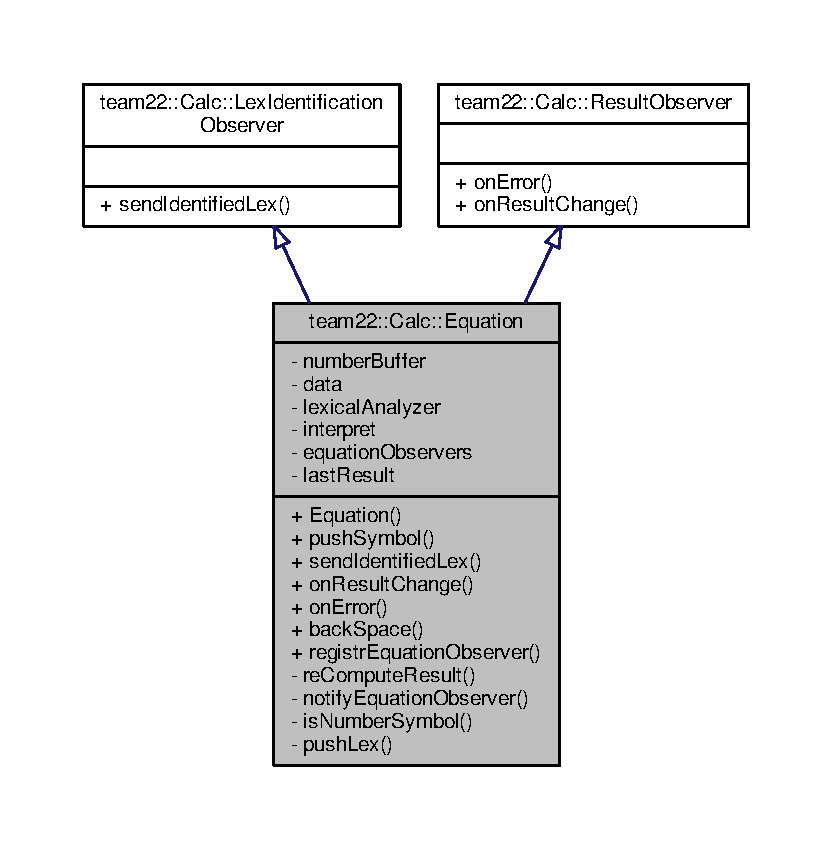
\includegraphics[width=350pt]{classteam22_1_1_calc_1_1_equation__inherit__graph}
\end{center}
\end{figure}


Collaboration diagram for team22\+:\+:Calc\+:\+:Equation\+:
\nopagebreak
\begin{figure}[H]
\begin{center}
\leavevmode
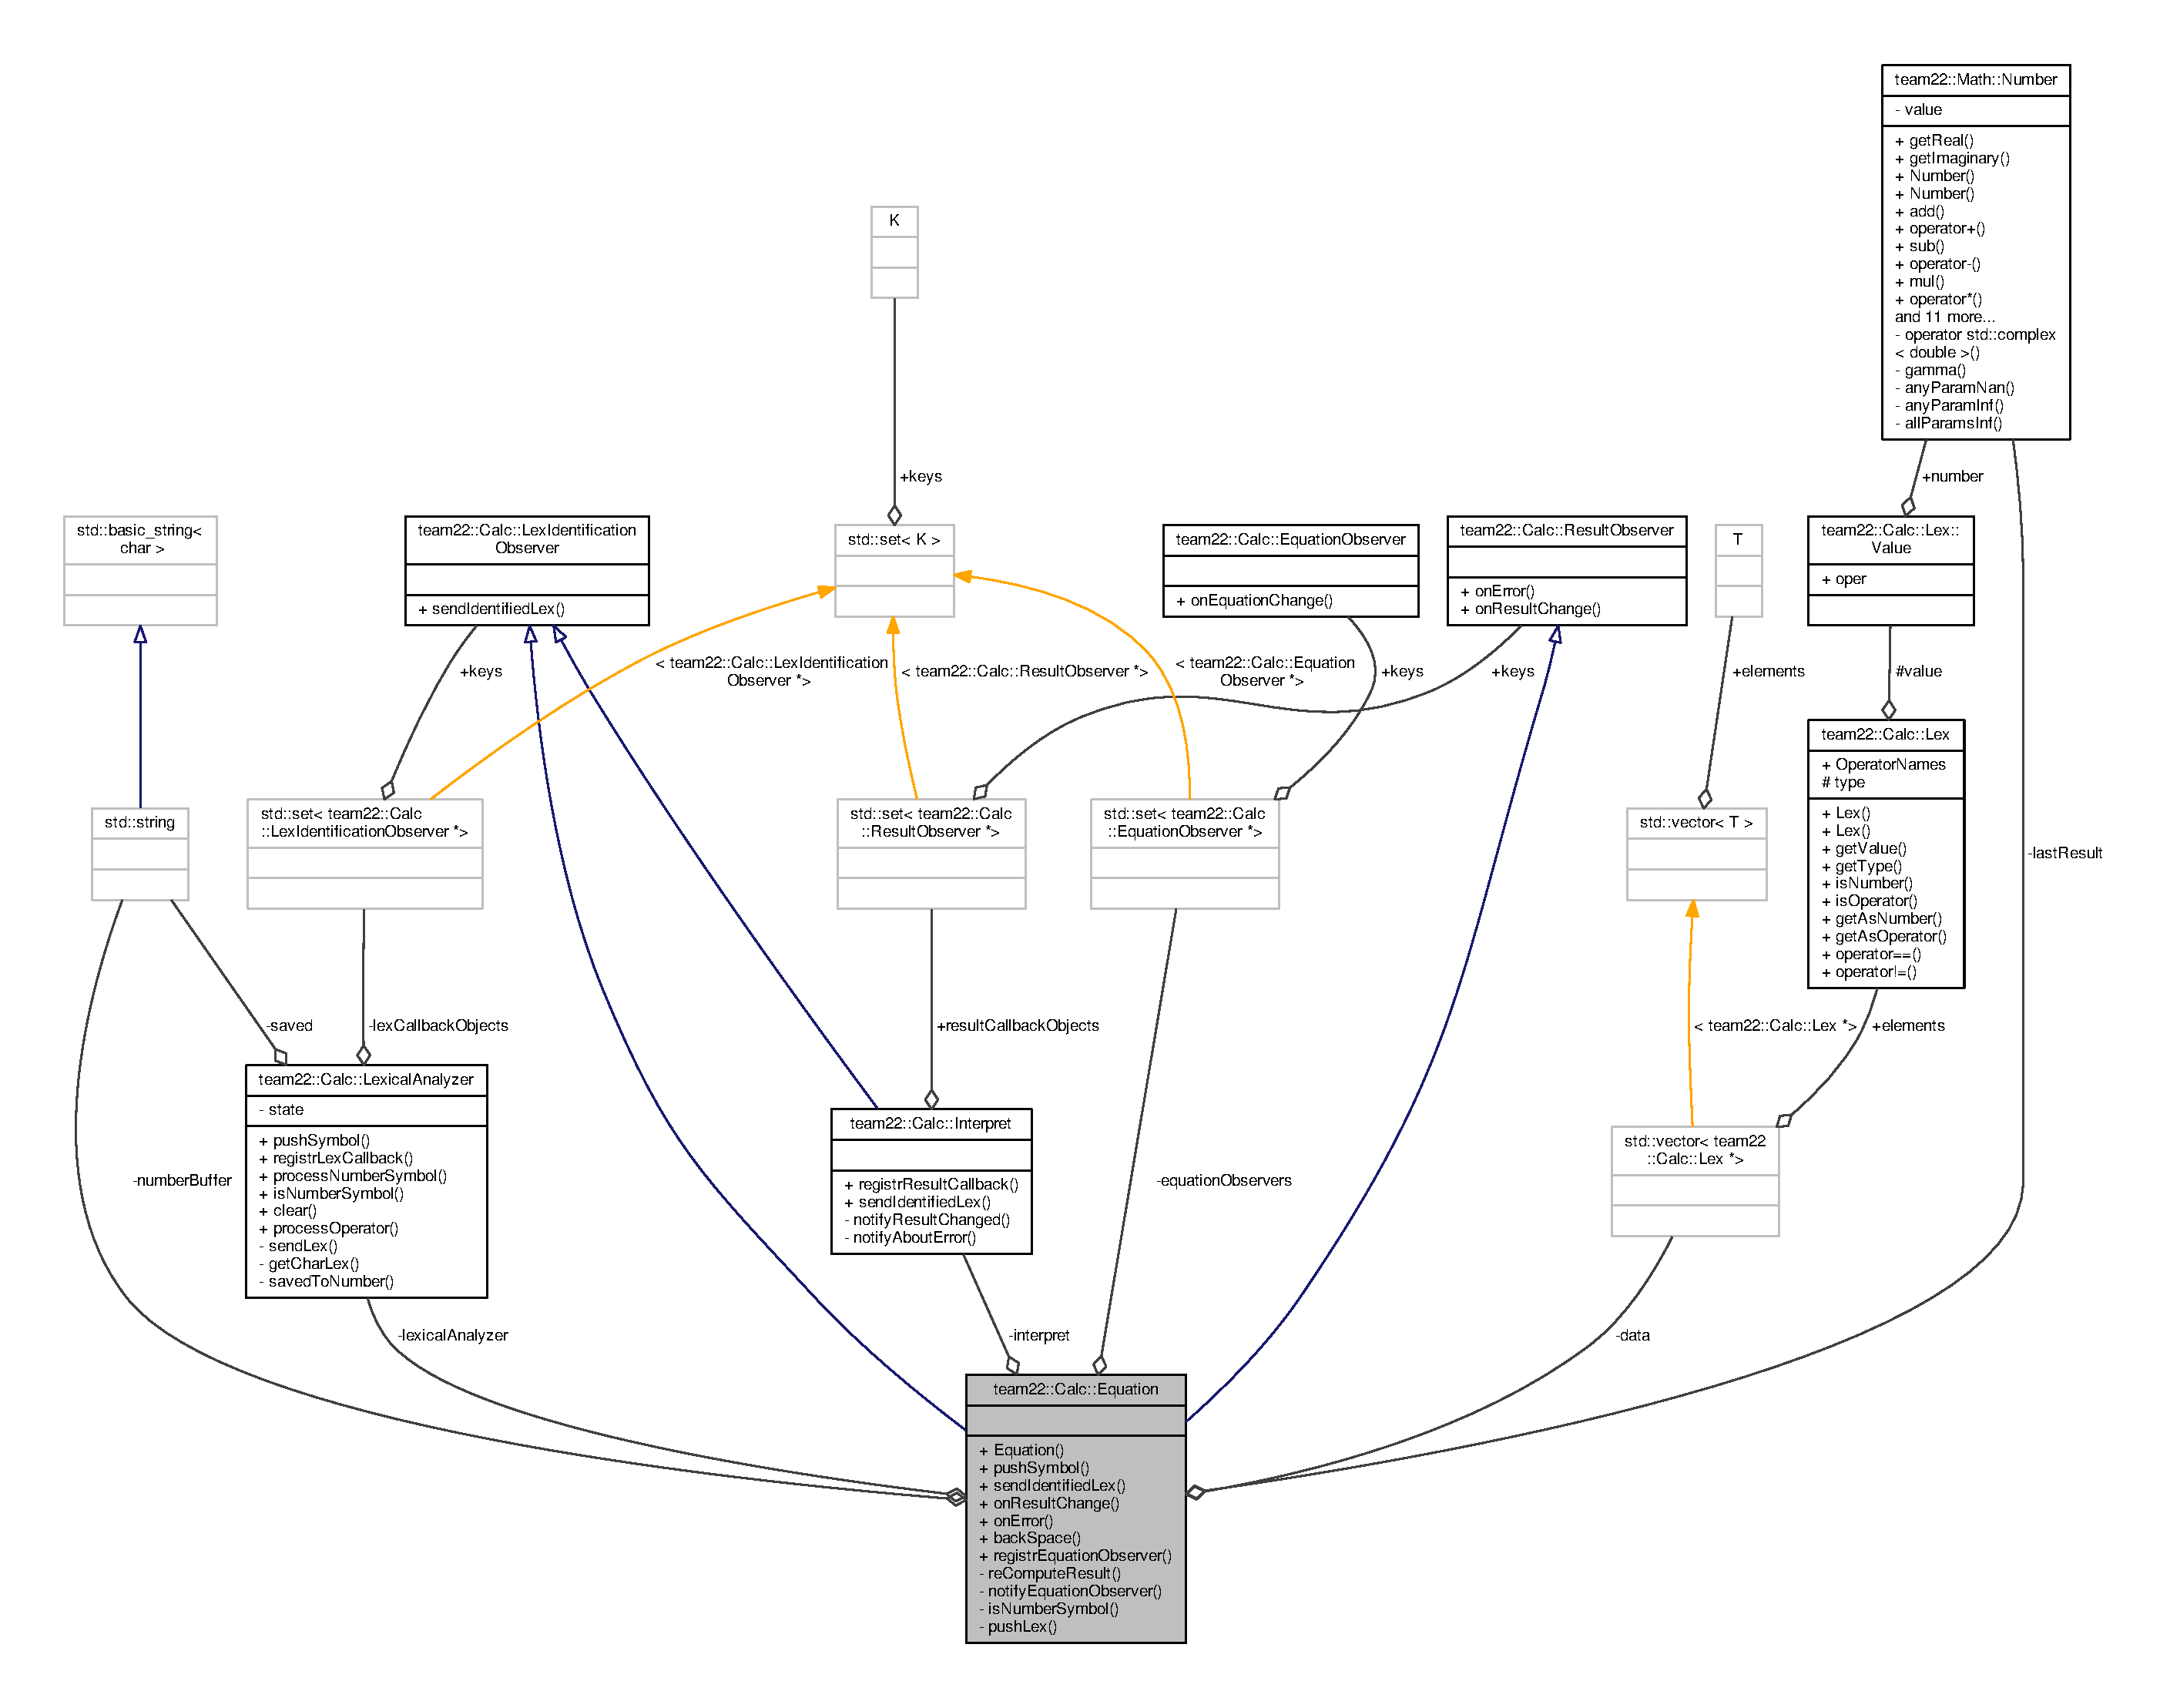
\includegraphics[width=350pt]{classteam22_1_1_calc_1_1_equation__coll__graph}
\end{center}
\end{figure}
\subsection*{Public Member Functions}
\begin{DoxyCompactItemize}
\item 
\hyperlink{classteam22_1_1_calc_1_1_equation_a085dc8be6e009511735b8c317d951610}{Equation} (\hyperlink{classteam22_1_1_calc_1_1_lexical_analyzer}{Lexical\+Analyzer} \&\hyperlink{classteam22_1_1_calc_1_1_equation_a65aeaa2a279994b03517a22addf31fc1}{lexical\+Analyzer}, \hyperlink{classteam22_1_1_calc_1_1_interpret}{Interpret} \&\hyperlink{classteam22_1_1_calc_1_1_equation_a8812a84e9c0f194eba491b0dba0cb015}{interpret})
\item 
void \hyperlink{classteam22_1_1_calc_1_1_equation_a324bf6372508c1b931c5ad8f39ccf8c4}{push\+Symbol} (char symbol)
\item 
void \hyperlink{classteam22_1_1_calc_1_1_equation_ad5768951865500ec7fc514f676de2851}{send\+Identified\+Lex} (\hyperlink{classteam22_1_1_calc_1_1_lex}{Lex} lex) override
\item 
void \hyperlink{classteam22_1_1_calc_1_1_equation_a302c295e099f589897a1bad4b02d3de8}{on\+Result\+Change} (\hyperlink{classteam22_1_1_math_1_1_number}{Math\+::\+Number} result) override
\item 
void \hyperlink{classteam22_1_1_calc_1_1_equation_a4e7a0614867931bcc714440441cdd894}{on\+Error} (\hyperlink{class_interpret_exception}{Interpret\+Exception} exception) override
\item 
void \hyperlink{classteam22_1_1_calc_1_1_equation_acccaaf8d823e6f1b7f6831fc0c8c4a62}{back\+Space} ()
\begin{DoxyCompactList}\small\item\em Provede operaci backspace Pokud je rovnice zakončena číslem odstraní poslední číslici jinak poslední lexem (operator) přepočítá rovnici. \end{DoxyCompactList}\item 
void \hyperlink{classteam22_1_1_calc_1_1_equation_a705c26d64f67f673e4919494d7e22d4a}{registr\+Equation\+Observer} (\hyperlink{classteam22_1_1_calc_1_1_equation_observer}{Equation\+Observer} $\ast$\hyperlink{classteam22_1_1_calc_1_1_equation_a76439666b11701dd1c42507397c5a316}{equation\+Observers})
\end{DoxyCompactItemize}
\subsection*{Private Member Functions}
\begin{DoxyCompactItemize}
\item 
void \hyperlink{classteam22_1_1_calc_1_1_equation_aba44b10dfb0ece96f3e0279d34cec868}{re\+Compute\+Result} ()
\item 
void \hyperlink{classteam22_1_1_calc_1_1_equation_acb90f7fefbd20c57864de0ed691bb65f}{notify\+Equation\+Observer} ()
\item 
bool \hyperlink{classteam22_1_1_calc_1_1_equation_afa4b44cfa408f74370851f7f64f55743}{is\+Number\+Symbol} (char \&symbol)
\item 
void \hyperlink{classteam22_1_1_calc_1_1_equation_af17ea6795813114d578e17109325d5e9}{push\+Lex} (\hyperlink{classteam22_1_1_calc_1_1_lex}{Lex} $\ast$lex)
\end{DoxyCompactItemize}
\subsection*{Private Attributes}
\begin{DoxyCompactItemize}
\item 
std\+::string \hyperlink{classteam22_1_1_calc_1_1_equation_a816d00b732bc472768b41da216a4335c}{number\+Buffer}
\item 
std\+::vector$<$ \hyperlink{classteam22_1_1_calc_1_1_lex}{Lex} $\ast$ $>$ \hyperlink{classteam22_1_1_calc_1_1_equation_ab02c12c6e452d5271f26bbae073ed4dc}{data}
\item 
\hyperlink{classteam22_1_1_calc_1_1_lexical_analyzer}{Lexical\+Analyzer} \hyperlink{classteam22_1_1_calc_1_1_equation_a65aeaa2a279994b03517a22addf31fc1}{lexical\+Analyzer}
\item 
\hyperlink{classteam22_1_1_calc_1_1_interpret}{Interpret} \hyperlink{classteam22_1_1_calc_1_1_equation_a8812a84e9c0f194eba491b0dba0cb015}{interpret}
\item 
std\+::set$<$ \hyperlink{classteam22_1_1_calc_1_1_equation_observer}{Equation\+Observer} $\ast$ $>$ \hyperlink{classteam22_1_1_calc_1_1_equation_a76439666b11701dd1c42507397c5a316}{equation\+Observers}
\item 
\hyperlink{classteam22_1_1_math_1_1_number}{Math\+::\+Number} \hyperlink{classteam22_1_1_calc_1_1_equation_a7c62440412a33b3b3300e63ff65ffafb}{last\+Result} = \{0\}
\end{DoxyCompactItemize}
\subsection*{Friends}
\begin{DoxyCompactItemize}
\item 
std\+::stringstream \& \hyperlink{classteam22_1_1_calc_1_1_equation_a8ee0e20eaa10e114d79e0b16cb11ddcf}{operator$<$$<$} (std\+::stringstream \&os, const \hyperlink{classteam22_1_1_calc_1_1_equation}{Equation} \&equation)
\item 
std\+::ostream \& \hyperlink{classteam22_1_1_calc_1_1_equation_aea7df9bdea5430cc309e17f1f2fbe78f}{operator$<$$<$} (std\+::ostream \&os, const \hyperlink{classteam22_1_1_calc_1_1_equation}{Equation} \&equation)
\end{DoxyCompactItemize}


\subsection{Detailed Description}
Třída reprezentující rovnici. 

Třída přebírá znaky a předává je Lexikálnímu analyzátoru, dále pozoruje Identifikaci Lexému. Při každé změně rovnice třída upozorní své pozorovatele o této změně. Pokud příjme lexem \hyperlink{classteam22_1_1_calc_1_1_lex_a61d29fc4878a3b36d2de2f13c56ed932ac62fe9cff8a15f20fb1416612309ae80}{Lex\+::\+BS} odebere číslici(i beru jako číslici) či operátor z konce rovnice a rovnici přepočítá Pokud příjme lexem \hyperlink{classteam22_1_1_calc_1_1_lex_a61d29fc4878a3b36d2de2f13c56ed932a4281d7ef6ac8dbf79c87603ca20c351c}{Lex\+::\+C\+L\+E\+AR} rovnice se smaže, Operátory \hyperlink{classteam22_1_1_calc_1_1_lex_a61d29fc4878a3b36d2de2f13c56ed932ac62fe9cff8a15f20fb1416612309ae80}{Lex\+::\+BS} \hyperlink{classteam22_1_1_calc_1_1_lex_a61d29fc4878a3b36d2de2f13c56ed932a4281d7ef6ac8dbf79c87603ca20c351c}{Lex\+::\+C\+L\+E\+AR} a \hyperlink{classteam22_1_1_calc_1_1_lex_a61d29fc4878a3b36d2de2f13c56ed932a3c1443c79523cadf6582f238c04a015f}{Lex\+::\+E\+V\+AL} se do rovnice nezapisují. Po \hyperlink{classteam22_1_1_calc_1_1_lex_a61d29fc4878a3b36d2de2f13c56ed932a3c1443c79523cadf6582f238c04a015f}{Lex\+::\+E\+V\+AL} pokud následuje číslo rovnice začíná tímto číslem a jinak začíná výsledkem předchozí rovnice pokud taková není 0. 

Definition at line 30 of file Equation.\+h.



\subsection{Constructor \& Destructor Documentation}
\mbox{\Hypertarget{classteam22_1_1_calc_1_1_equation_a085dc8be6e009511735b8c317d951610}\label{classteam22_1_1_calc_1_1_equation_a085dc8be6e009511735b8c317d951610}} 
\index{team22\+::\+Calc\+::\+Equation@{team22\+::\+Calc\+::\+Equation}!Equation@{Equation}}
\index{Equation@{Equation}!team22\+::\+Calc\+::\+Equation@{team22\+::\+Calc\+::\+Equation}}
\subsubsection{\texorpdfstring{Equation()}{Equation()}}
{\footnotesize\ttfamily Equation\+::\+Equation (\begin{DoxyParamCaption}\item[{\hyperlink{classteam22_1_1_calc_1_1_lexical_analyzer}{Lexical\+Analyzer} \&}]{lexical\+Analyzer,  }\item[{\hyperlink{classteam22_1_1_calc_1_1_interpret}{Interpret} \&}]{interpret }\end{DoxyParamCaption})}


\begin{DoxyParams}{Parameters}
{\em lexical\+Analyzer} & \\
\hline
{\em interpret} & \\
\hline
\end{DoxyParams}


Definition at line 106 of file Equation.\+cpp.



References team22\+::\+Calc\+::\+Lexical\+Analyzer\+::registr\+Lex\+Callback().



\subsection{Member Function Documentation}
\mbox{\Hypertarget{classteam22_1_1_calc_1_1_equation_acccaaf8d823e6f1b7f6831fc0c8c4a62}\label{classteam22_1_1_calc_1_1_equation_acccaaf8d823e6f1b7f6831fc0c8c4a62}} 
\index{team22\+::\+Calc\+::\+Equation@{team22\+::\+Calc\+::\+Equation}!back\+Space@{back\+Space}}
\index{back\+Space@{back\+Space}!team22\+::\+Calc\+::\+Equation@{team22\+::\+Calc\+::\+Equation}}
\subsubsection{\texorpdfstring{back\+Space()}{backSpace()}}
{\footnotesize\ttfamily void Equation\+::back\+Space (\begin{DoxyParamCaption}{ }\end{DoxyParamCaption})}



Provede operaci backspace Pokud je rovnice zakončena číslem odstraní poslední číslici jinak poslední lexem (operator) přepočítá rovnici. 



Definition at line 56 of file Equation.\+cpp.



References data, lexical\+Analyzer, number\+Buffer, team22\+::\+Calc\+::\+Lexical\+Analyzer\+::push\+Symbol(), and re\+Compute\+Result().



Referenced by send\+Identified\+Lex().

\mbox{\Hypertarget{classteam22_1_1_calc_1_1_equation_afa4b44cfa408f74370851f7f64f55743}\label{classteam22_1_1_calc_1_1_equation_afa4b44cfa408f74370851f7f64f55743}} 
\index{team22\+::\+Calc\+::\+Equation@{team22\+::\+Calc\+::\+Equation}!is\+Number\+Symbol@{is\+Number\+Symbol}}
\index{is\+Number\+Symbol@{is\+Number\+Symbol}!team22\+::\+Calc\+::\+Equation@{team22\+::\+Calc\+::\+Equation}}
\subsubsection{\texorpdfstring{is\+Number\+Symbol()}{isNumberSymbol()}}
{\footnotesize\ttfamily bool Equation\+::is\+Number\+Symbol (\begin{DoxyParamCaption}\item[{char \&}]{symbol }\end{DoxyParamCaption})\hspace{0.3cm}{\ttfamily [private]}}

Jedná se o znak čísla tedy číslici nebo i 

Definition at line 95 of file Equation.\+cpp.



Referenced by push\+Symbol().

\mbox{\Hypertarget{classteam22_1_1_calc_1_1_equation_acb90f7fefbd20c57864de0ed691bb65f}\label{classteam22_1_1_calc_1_1_equation_acb90f7fefbd20c57864de0ed691bb65f}} 
\index{team22\+::\+Calc\+::\+Equation@{team22\+::\+Calc\+::\+Equation}!notify\+Equation\+Observer@{notify\+Equation\+Observer}}
\index{notify\+Equation\+Observer@{notify\+Equation\+Observer}!team22\+::\+Calc\+::\+Equation@{team22\+::\+Calc\+::\+Equation}}
\subsubsection{\texorpdfstring{notify\+Equation\+Observer()}{notifyEquationObserver()}}
{\footnotesize\ttfamily void Equation\+::notify\+Equation\+Observer (\begin{DoxyParamCaption}{ }\end{DoxyParamCaption})\hspace{0.3cm}{\ttfamily [private]}}

upozorní odebíratele na změnu rovnice 

Definition at line 89 of file Equation.\+cpp.



References equation\+Observers.



Referenced by push\+Symbol(), and send\+Identified\+Lex().

\mbox{\Hypertarget{classteam22_1_1_calc_1_1_equation_a4e7a0614867931bcc714440441cdd894}\label{classteam22_1_1_calc_1_1_equation_a4e7a0614867931bcc714440441cdd894}} 
\index{team22\+::\+Calc\+::\+Equation@{team22\+::\+Calc\+::\+Equation}!on\+Error@{on\+Error}}
\index{on\+Error@{on\+Error}!team22\+::\+Calc\+::\+Equation@{team22\+::\+Calc\+::\+Equation}}
\subsubsection{\texorpdfstring{on\+Error()}{onError()}}
{\footnotesize\ttfamily void Equation\+::on\+Error (\begin{DoxyParamCaption}\item[{\hyperlink{class_interpret_exception}{Interpret\+Exception}}]{exception }\end{DoxyParamCaption})\hspace{0.3cm}{\ttfamily [override]}, {\ttfamily [virtual]}}


\begin{DoxyParams}{Parameters}
{\em exception} & \\
\hline
\end{DoxyParams}


Implements \hyperlink{classteam22_1_1_calc_1_1_result_observer_ad36cf8df89853d60f91094800c01d329}{team22\+::\+Calc\+::\+Result\+Observer}.



Definition at line 122 of file Equation.\+cpp.



References data, and number\+Buffer.

\mbox{\Hypertarget{classteam22_1_1_calc_1_1_equation_a302c295e099f589897a1bad4b02d3de8}\label{classteam22_1_1_calc_1_1_equation_a302c295e099f589897a1bad4b02d3de8}} 
\index{team22\+::\+Calc\+::\+Equation@{team22\+::\+Calc\+::\+Equation}!on\+Result\+Change@{on\+Result\+Change}}
\index{on\+Result\+Change@{on\+Result\+Change}!team22\+::\+Calc\+::\+Equation@{team22\+::\+Calc\+::\+Equation}}
\subsubsection{\texorpdfstring{on\+Result\+Change()}{onResultChange()}}
{\footnotesize\ttfamily void Equation\+::on\+Result\+Change (\begin{DoxyParamCaption}\item[{\hyperlink{classteam22_1_1_math_1_1_number}{Math\+::\+Number}}]{result }\end{DoxyParamCaption})\hspace{0.3cm}{\ttfamily [override]}, {\ttfamily [virtual]}}


\begin{DoxyParams}{Parameters}
{\em result} & \\
\hline
\end{DoxyParams}


Implements \hyperlink{classteam22_1_1_calc_1_1_result_observer_aa04007df3aa8a499c3a511f549238285}{team22\+::\+Calc\+::\+Result\+Observer}.



Definition at line 117 of file Equation.\+cpp.



References last\+Result.

\mbox{\Hypertarget{classteam22_1_1_calc_1_1_equation_af17ea6795813114d578e17109325d5e9}\label{classteam22_1_1_calc_1_1_equation_af17ea6795813114d578e17109325d5e9}} 
\index{team22\+::\+Calc\+::\+Equation@{team22\+::\+Calc\+::\+Equation}!push\+Lex@{push\+Lex}}
\index{push\+Lex@{push\+Lex}!team22\+::\+Calc\+::\+Equation@{team22\+::\+Calc\+::\+Equation}}
\subsubsection{\texorpdfstring{push\+Lex()}{pushLex()}}
{\footnotesize\ttfamily void Equation\+::push\+Lex (\begin{DoxyParamCaption}\item[{\hyperlink{classteam22_1_1_calc_1_1_lex}{Lex} $\ast$}]{lex }\end{DoxyParamCaption})\hspace{0.3cm}{\ttfamily [private]}}

zpracuje příchozí Lexém 
\begin{DoxyParams}{Parameters}
{\em lex} & \\
\hline
\end{DoxyParams}


Definition at line 112 of file Equation.\+cpp.



References data.



Referenced by send\+Identified\+Lex().

\mbox{\Hypertarget{classteam22_1_1_calc_1_1_equation_a324bf6372508c1b931c5ad8f39ccf8c4}\label{classteam22_1_1_calc_1_1_equation_a324bf6372508c1b931c5ad8f39ccf8c4}} 
\index{team22\+::\+Calc\+::\+Equation@{team22\+::\+Calc\+::\+Equation}!push\+Symbol@{push\+Symbol}}
\index{push\+Symbol@{push\+Symbol}!team22\+::\+Calc\+::\+Equation@{team22\+::\+Calc\+::\+Equation}}
\subsubsection{\texorpdfstring{push\+Symbol()}{pushSymbol()}}
{\footnotesize\ttfamily void Equation\+::push\+Symbol (\begin{DoxyParamCaption}\item[{char}]{symbol }\end{DoxyParamCaption})}

Předání symbolu rovnici 
\begin{DoxyExceptions}{Exceptions}
{\em \hyperlink{classteam22_1_1_calc_1_1_lexical_analyzer_exception}{Lexical\+Analyzer\+Exception}} & \\
\hline
\end{DoxyExceptions}


Definition at line 45 of file Equation.\+cpp.



References is\+Number\+Symbol(), lexical\+Analyzer, notify\+Equation\+Observer(), number\+Buffer, and team22\+::\+Calc\+::\+Lexical\+Analyzer\+::push\+Symbol().



Referenced by T\+E\+S\+T().

\mbox{\Hypertarget{classteam22_1_1_calc_1_1_equation_aba44b10dfb0ece96f3e0279d34cec868}\label{classteam22_1_1_calc_1_1_equation_aba44b10dfb0ece96f3e0279d34cec868}} 
\index{team22\+::\+Calc\+::\+Equation@{team22\+::\+Calc\+::\+Equation}!re\+Compute\+Result@{re\+Compute\+Result}}
\index{re\+Compute\+Result@{re\+Compute\+Result}!team22\+::\+Calc\+::\+Equation@{team22\+::\+Calc\+::\+Equation}}
\subsubsection{\texorpdfstring{re\+Compute\+Result()}{reComputeResult()}}
{\footnotesize\ttfamily void Equation\+::re\+Compute\+Result (\begin{DoxyParamCaption}{ }\end{DoxyParamCaption})\hspace{0.3cm}{\ttfamily [private]}}

přepočítá výsledek 

Definition at line 100 of file Equation.\+cpp.



References data, interpret, and team22\+::\+Calc\+::\+Interpret\+::send\+Identified\+Lex().



Referenced by back\+Space().

\mbox{\Hypertarget{classteam22_1_1_calc_1_1_equation_a705c26d64f67f673e4919494d7e22d4a}\label{classteam22_1_1_calc_1_1_equation_a705c26d64f67f673e4919494d7e22d4a}} 
\index{team22\+::\+Calc\+::\+Equation@{team22\+::\+Calc\+::\+Equation}!registr\+Equation\+Observer@{registr\+Equation\+Observer}}
\index{registr\+Equation\+Observer@{registr\+Equation\+Observer}!team22\+::\+Calc\+::\+Equation@{team22\+::\+Calc\+::\+Equation}}
\subsubsection{\texorpdfstring{registr\+Equation\+Observer()}{registrEquationObserver()}}
{\footnotesize\ttfamily void Equation\+::registr\+Equation\+Observer (\begin{DoxyParamCaption}\item[{\hyperlink{classteam22_1_1_calc_1_1_equation_observer}{Equation\+Observer} $\ast$}]{equation\+Observers }\end{DoxyParamCaption})}

Zaregistruje pozorovatele změny rovnice 
\begin{DoxyParams}{Parameters}
{\em equation\+Observers} & \\
\hline
\end{DoxyParams}


Definition at line 84 of file Equation.\+cpp.



References equation\+Observers.



Referenced by Backend\+Tester\+::\+Backend\+Tester().

\mbox{\Hypertarget{classteam22_1_1_calc_1_1_equation_ad5768951865500ec7fc514f676de2851}\label{classteam22_1_1_calc_1_1_equation_ad5768951865500ec7fc514f676de2851}} 
\index{team22\+::\+Calc\+::\+Equation@{team22\+::\+Calc\+::\+Equation}!send\+Identified\+Lex@{send\+Identified\+Lex}}
\index{send\+Identified\+Lex@{send\+Identified\+Lex}!team22\+::\+Calc\+::\+Equation@{team22\+::\+Calc\+::\+Equation}}
\subsubsection{\texorpdfstring{send\+Identified\+Lex()}{sendIdentifiedLex()}}
{\footnotesize\ttfamily void Equation\+::send\+Identified\+Lex (\begin{DoxyParamCaption}\item[{\hyperlink{classteam22_1_1_calc_1_1_lex}{Lex}}]{lex }\end{DoxyParamCaption})\hspace{0.3cm}{\ttfamily [override]}, {\ttfamily [virtual]}}


\begin{DoxyParams}{Parameters}
{\em lex} & \\
\hline
\end{DoxyParams}


Implements \hyperlink{classteam22_1_1_calc_1_1_lex_identification_observer_ac139f75c560625ec6fdb2e34cf0d4884}{team22\+::\+Calc\+::\+Lex\+Identification\+Observer}.



Definition at line 15 of file Equation.\+cpp.



References back\+Space(), team22\+::\+Calc\+::\+Lex\+::\+BS, team22\+::\+Calc\+::\+Lex\+::\+C\+L\+E\+AR, data, team22\+::\+Calc\+::\+Lex\+::\+E\+V\+AL, team22\+::\+Calc\+::\+Lex\+::get\+As\+Operator(), interpret, team22\+::\+Calc\+::\+Lex\+::is\+Operator(), last\+Result, notify\+Equation\+Observer(), number\+Buffer, push\+Lex(), and team22\+::\+Calc\+::\+Interpret\+::send\+Identified\+Lex().



\subsection{Friends And Related Function Documentation}
\mbox{\Hypertarget{classteam22_1_1_calc_1_1_equation_a8ee0e20eaa10e114d79e0b16cb11ddcf}\label{classteam22_1_1_calc_1_1_equation_a8ee0e20eaa10e114d79e0b16cb11ddcf}} 
\index{team22\+::\+Calc\+::\+Equation@{team22\+::\+Calc\+::\+Equation}!operator$<$$<$@{operator$<$$<$}}
\index{operator$<$$<$@{operator$<$$<$}!team22\+::\+Calc\+::\+Equation@{team22\+::\+Calc\+::\+Equation}}
\subsubsection{\texorpdfstring{operator$<$$<$}{operator<<}\hspace{0.1cm}{\footnotesize\ttfamily [1/2]}}
{\footnotesize\ttfamily std\+::stringstream\& operator$<$$<$ (\begin{DoxyParamCaption}\item[{std\+::stringstream \&}]{os,  }\item[{const \hyperlink{classteam22_1_1_calc_1_1_equation}{Equation} \&}]{equation }\end{DoxyParamCaption})\hspace{0.3cm}{\ttfamily [friend]}}

\mbox{\Hypertarget{classteam22_1_1_calc_1_1_equation_aea7df9bdea5430cc309e17f1f2fbe78f}\label{classteam22_1_1_calc_1_1_equation_aea7df9bdea5430cc309e17f1f2fbe78f}} 
\index{team22\+::\+Calc\+::\+Equation@{team22\+::\+Calc\+::\+Equation}!operator$<$$<$@{operator$<$$<$}}
\index{operator$<$$<$@{operator$<$$<$}!team22\+::\+Calc\+::\+Equation@{team22\+::\+Calc\+::\+Equation}}
\subsubsection{\texorpdfstring{operator$<$$<$}{operator<<}\hspace{0.1cm}{\footnotesize\ttfamily [2/2]}}
{\footnotesize\ttfamily std\+::ostream\& operator$<$$<$ (\begin{DoxyParamCaption}\item[{std\+::ostream \&}]{os,  }\item[{const \hyperlink{classteam22_1_1_calc_1_1_equation}{Equation} \&}]{equation }\end{DoxyParamCaption})\hspace{0.3cm}{\ttfamily [friend]}}



\subsection{Member Data Documentation}
\mbox{\Hypertarget{classteam22_1_1_calc_1_1_equation_ab02c12c6e452d5271f26bbae073ed4dc}\label{classteam22_1_1_calc_1_1_equation_ab02c12c6e452d5271f26bbae073ed4dc}} 
\index{team22\+::\+Calc\+::\+Equation@{team22\+::\+Calc\+::\+Equation}!data@{data}}
\index{data@{data}!team22\+::\+Calc\+::\+Equation@{team22\+::\+Calc\+::\+Equation}}
\subsubsection{\texorpdfstring{data}{data}}
{\footnotesize\ttfamily std\+::vector$<$\hyperlink{classteam22_1_1_calc_1_1_lex}{Lex} $\ast$$>$ team22\+::\+Calc\+::\+Equation\+::data\hspace{0.3cm}{\ttfamily [private]}}

Lexémy tvořící rovnici 

Definition at line 42 of file Equation.\+h.



Referenced by back\+Space(), on\+Error(), push\+Lex(), re\+Compute\+Result(), and send\+Identified\+Lex().

\mbox{\Hypertarget{classteam22_1_1_calc_1_1_equation_a76439666b11701dd1c42507397c5a316}\label{classteam22_1_1_calc_1_1_equation_a76439666b11701dd1c42507397c5a316}} 
\index{team22\+::\+Calc\+::\+Equation@{team22\+::\+Calc\+::\+Equation}!equation\+Observers@{equation\+Observers}}
\index{equation\+Observers@{equation\+Observers}!team22\+::\+Calc\+::\+Equation@{team22\+::\+Calc\+::\+Equation}}
\subsubsection{\texorpdfstring{equation\+Observers}{equationObservers}}
{\footnotesize\ttfamily std\+::set$<$\hyperlink{classteam22_1_1_calc_1_1_equation_observer}{Equation\+Observer} $\ast$$>$ team22\+::\+Calc\+::\+Equation\+::equation\+Observers\hspace{0.3cm}{\ttfamily [private]}}

Pozorovatele 

Definition at line 59 of file Equation.\+h.



Referenced by notify\+Equation\+Observer(), and registr\+Equation\+Observer().

\mbox{\Hypertarget{classteam22_1_1_calc_1_1_equation_a8812a84e9c0f194eba491b0dba0cb015}\label{classteam22_1_1_calc_1_1_equation_a8812a84e9c0f194eba491b0dba0cb015}} 
\index{team22\+::\+Calc\+::\+Equation@{team22\+::\+Calc\+::\+Equation}!interpret@{interpret}}
\index{interpret@{interpret}!team22\+::\+Calc\+::\+Equation@{team22\+::\+Calc\+::\+Equation}}
\subsubsection{\texorpdfstring{interpret}{interpret}}
{\footnotesize\ttfamily \hyperlink{classteam22_1_1_calc_1_1_interpret}{Interpret} team22\+::\+Calc\+::\+Equation\+::interpret\hspace{0.3cm}{\ttfamily [private]}}

\hyperlink{classteam22_1_1_calc_1_1_interpret}{Interpret} 

Definition at line 54 of file Equation.\+h.



Referenced by re\+Compute\+Result(), and send\+Identified\+Lex().

\mbox{\Hypertarget{classteam22_1_1_calc_1_1_equation_a7c62440412a33b3b3300e63ff65ffafb}\label{classteam22_1_1_calc_1_1_equation_a7c62440412a33b3b3300e63ff65ffafb}} 
\index{team22\+::\+Calc\+::\+Equation@{team22\+::\+Calc\+::\+Equation}!last\+Result@{last\+Result}}
\index{last\+Result@{last\+Result}!team22\+::\+Calc\+::\+Equation@{team22\+::\+Calc\+::\+Equation}}
\subsubsection{\texorpdfstring{last\+Result}{lastResult}}
{\footnotesize\ttfamily \hyperlink{classteam22_1_1_math_1_1_number}{Math\+::\+Number} team22\+::\+Calc\+::\+Equation\+::last\+Result = \{0\}\hspace{0.3cm}{\ttfamily [private]}}

Poslední výsledek rovnice 

Definition at line 64 of file Equation.\+h.



Referenced by on\+Result\+Change(), and send\+Identified\+Lex().

\mbox{\Hypertarget{classteam22_1_1_calc_1_1_equation_a65aeaa2a279994b03517a22addf31fc1}\label{classteam22_1_1_calc_1_1_equation_a65aeaa2a279994b03517a22addf31fc1}} 
\index{team22\+::\+Calc\+::\+Equation@{team22\+::\+Calc\+::\+Equation}!lexical\+Analyzer@{lexical\+Analyzer}}
\index{lexical\+Analyzer@{lexical\+Analyzer}!team22\+::\+Calc\+::\+Equation@{team22\+::\+Calc\+::\+Equation}}
\subsubsection{\texorpdfstring{lexical\+Analyzer}{lexicalAnalyzer}}
{\footnotesize\ttfamily \hyperlink{classteam22_1_1_calc_1_1_lexical_analyzer}{Lexical\+Analyzer} team22\+::\+Calc\+::\+Equation\+::lexical\+Analyzer\hspace{0.3cm}{\ttfamily [private]}}

Lexikální analyzátor 

Definition at line 49 of file Equation.\+h.



Referenced by back\+Space(), and push\+Symbol().

\mbox{\Hypertarget{classteam22_1_1_calc_1_1_equation_a816d00b732bc472768b41da216a4335c}\label{classteam22_1_1_calc_1_1_equation_a816d00b732bc472768b41da216a4335c}} 
\index{team22\+::\+Calc\+::\+Equation@{team22\+::\+Calc\+::\+Equation}!number\+Buffer@{number\+Buffer}}
\index{number\+Buffer@{number\+Buffer}!team22\+::\+Calc\+::\+Equation@{team22\+::\+Calc\+::\+Equation}}
\subsubsection{\texorpdfstring{number\+Buffer}{numberBuffer}}
{\footnotesize\ttfamily std\+::string team22\+::\+Calc\+::\+Equation\+::number\+Buffer\hspace{0.3cm}{\ttfamily [private]}}

Buffer pro rozepsané číslo číslo v rovnici chceme zobrazovat ješte předním, než je celé identifikováno jako lexem k tomu nám pomáhá tento buffer. 

Definition at line 37 of file Equation.\+h.



Referenced by back\+Space(), on\+Error(), push\+Symbol(), and send\+Identified\+Lex().



The documentation for this class was generated from the following files\+:\begin{DoxyCompactItemize}
\item 
src/\hyperlink{_equation_8h}{Equation.\+h}\item 
src/\hyperlink{_equation_8cpp}{Equation.\+cpp}\end{DoxyCompactItemize}

\hypertarget{classteam22_1_1_calc_1_1_equation_observer}{}\section{team22\+:\+:Calc\+:\+:Equation\+Observer Class Reference}
\label{classteam22_1_1_calc_1_1_equation_observer}\index{team22\+::\+Calc\+::\+Equation\+Observer@{team22\+::\+Calc\+::\+Equation\+Observer}}


{\ttfamily \#include $<$Equation\+Observer.\+h$>$}



Inheritance diagram for team22\+:\+:Calc\+:\+:Equation\+Observer\+:
\nopagebreak
\begin{figure}[H]
\begin{center}
\leavevmode
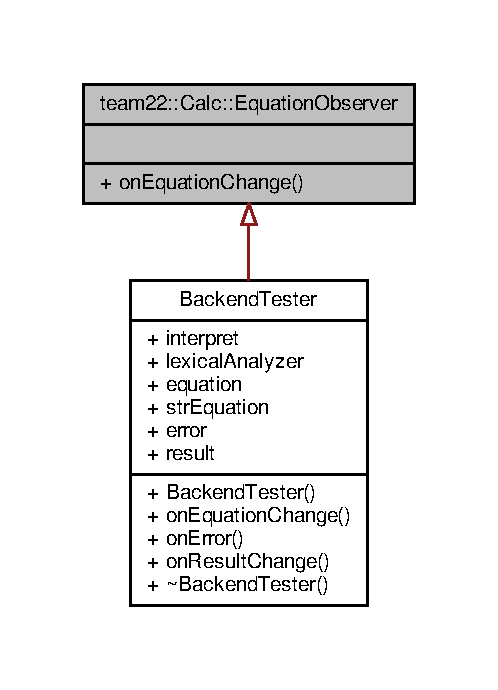
\includegraphics[width=239pt]{classteam22_1_1_calc_1_1_equation_observer__inherit__graph}
\end{center}
\end{figure}


Collaboration diagram for team22\+:\+:Calc\+:\+:Equation\+Observer\+:
\nopagebreak
\begin{figure}[H]
\begin{center}
\leavevmode
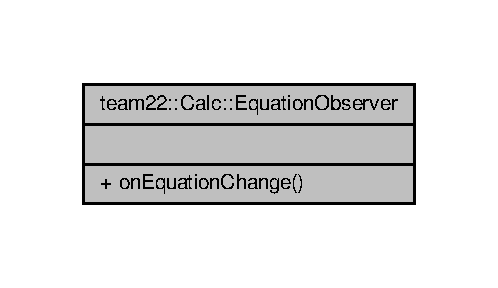
\includegraphics[width=239pt]{classteam22_1_1_calc_1_1_equation_observer__coll__graph}
\end{center}
\end{figure}
\subsection*{Public Member Functions}
\begin{DoxyCompactItemize}
\item 
virtual void \hyperlink{classteam22_1_1_calc_1_1_equation_observer_a2fc2a1f8583f27b0087ff6053895ef25}{on\+Equation\+Change} ()=0
\end{DoxyCompactItemize}


\subsection{Detailed Description}


Definition at line 12 of file Equation\+Observer.\+h.



\subsection{Member Function Documentation}
\mbox{\Hypertarget{classteam22_1_1_calc_1_1_equation_observer_a2fc2a1f8583f27b0087ff6053895ef25}\label{classteam22_1_1_calc_1_1_equation_observer_a2fc2a1f8583f27b0087ff6053895ef25}} 
\index{team22\+::\+Calc\+::\+Equation\+Observer@{team22\+::\+Calc\+::\+Equation\+Observer}!on\+Equation\+Change@{on\+Equation\+Change}}
\index{on\+Equation\+Change@{on\+Equation\+Change}!team22\+::\+Calc\+::\+Equation\+Observer@{team22\+::\+Calc\+::\+Equation\+Observer}}
\subsubsection{\texorpdfstring{on\+Equation\+Change()}{onEquationChange()}}
{\footnotesize\ttfamily virtual void team22\+::\+Calc\+::\+Equation\+Observer\+::on\+Equation\+Change (\begin{DoxyParamCaption}{ }\end{DoxyParamCaption})\hspace{0.3cm}{\ttfamily [pure virtual]}}



Implemented in \hyperlink{class_backend_tester_a9b7caf17f8ad274936fab5ca4bc669f8}{Backend\+Tester}.



The documentation for this class was generated from the following file\+:\begin{DoxyCompactItemize}
\item 
src/\hyperlink{_equation_observer_8h}{Equation\+Observer.\+h}\end{DoxyCompactItemize}

\hypertarget{classteam22_1_1_calc_1_1_interpret}{}\section{team22\+:\+:Calc\+:\+:Interpret Class Reference}
\label{classteam22_1_1_calc_1_1_interpret}\index{team22\+::\+Calc\+::\+Interpret@{team22\+::\+Calc\+::\+Interpret}}


{\ttfamily \#include $<$Interpret.\+h$>$}



Inheritance diagram for team22\+:\+:Calc\+:\+:Interpret\+:
\nopagebreak
\begin{figure}[H]
\begin{center}
\leavevmode
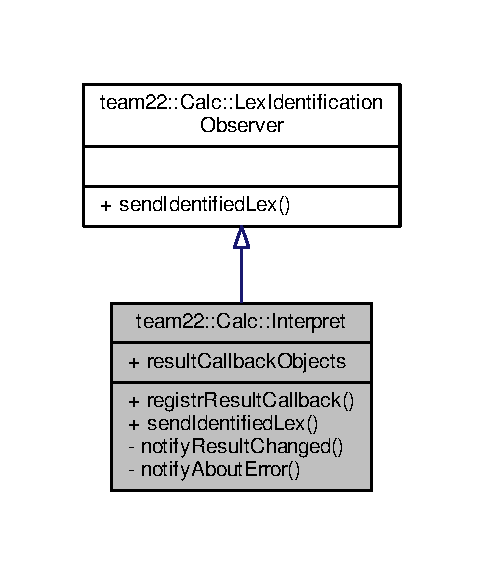
\includegraphics[width=232pt]{classteam22_1_1_calc_1_1_interpret__inherit__graph}
\end{center}
\end{figure}


Collaboration diagram for team22\+:\+:Calc\+:\+:Interpret\+:
\nopagebreak
\begin{figure}[H]
\begin{center}
\leavevmode
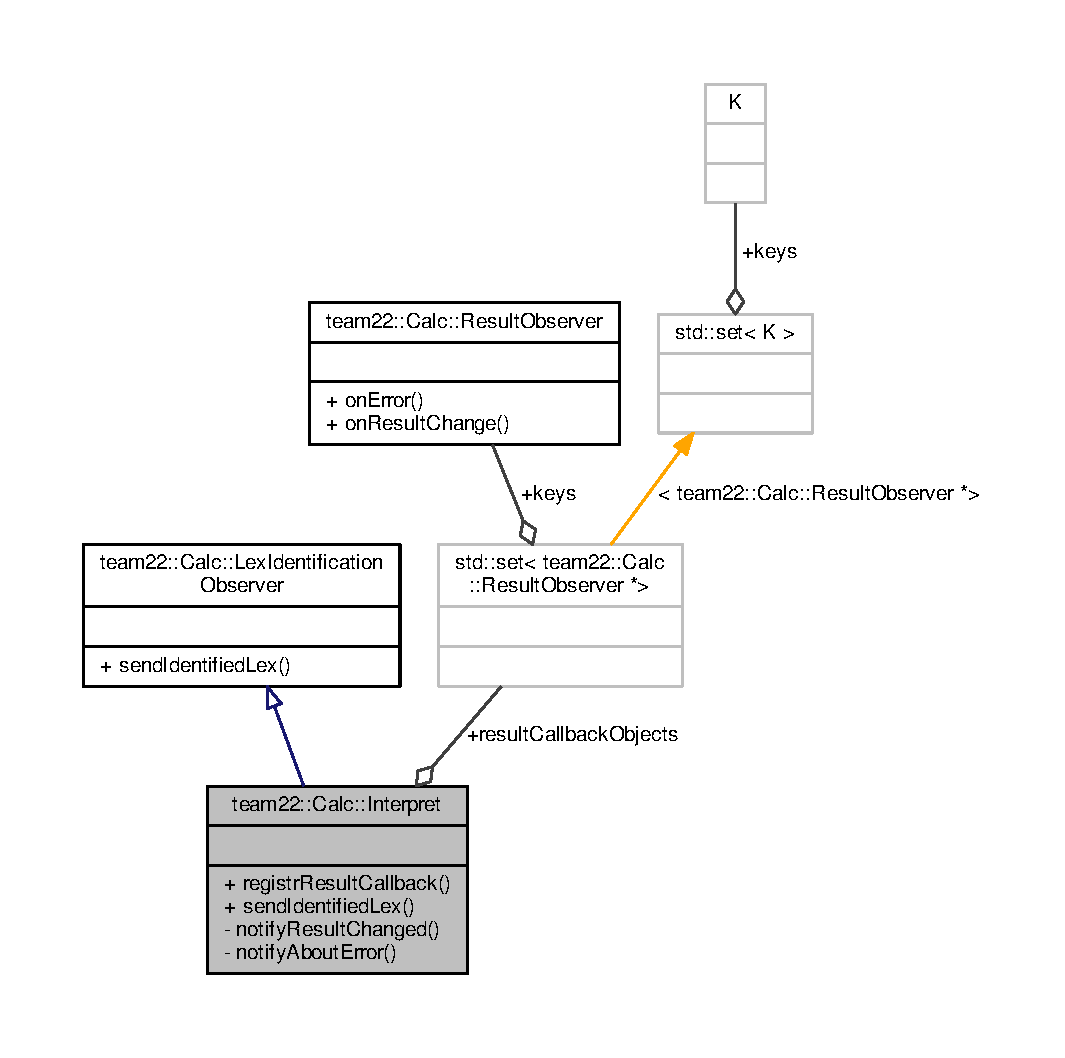
\includegraphics[width=350pt]{classteam22_1_1_calc_1_1_interpret__coll__graph}
\end{center}
\end{figure}
\subsection*{Public Member Functions}
\begin{DoxyCompactItemize}
\item 
void \hyperlink{classteam22_1_1_calc_1_1_interpret_a23e1e307b4f7ffd42f8eb31d33314c41}{registr\+Result\+Callback} (\hyperlink{classteam22_1_1_calc_1_1_result_observer}{Result\+Observer} $\ast$result\+Callback\+Object)
\item 
void \hyperlink{classteam22_1_1_calc_1_1_interpret_a479c65c010f4ef1060049b684e5f7eb6}{send\+Identified\+Lex} (\hyperlink{classteam22_1_1_calc_1_1_lex}{Lex} lex) override
\end{DoxyCompactItemize}
\subsection*{Public Attributes}
\begin{DoxyCompactItemize}
\item 
std\+::set$<$ \hyperlink{classteam22_1_1_calc_1_1_result_observer}{Result\+Observer} $\ast$ $>$ \hyperlink{classteam22_1_1_calc_1_1_interpret_a7db1e80a4733124ed425e62a90f9eadb}{result\+Callback\+Objects}
\end{DoxyCompactItemize}
\subsection*{Private Member Functions}
\begin{DoxyCompactItemize}
\item 
void \hyperlink{classteam22_1_1_calc_1_1_interpret_af38e3b867c32f50c921027249fc1185a}{notify\+Result\+Changed} ()
\item 
void \hyperlink{classteam22_1_1_calc_1_1_interpret_ab9db5790b1aab8a3f315296853c8e9c6}{notify\+About\+Error} (\hyperlink{class_interpret_exception}{Interpret\+Exception} exception)
\end{DoxyCompactItemize}


\subsection{Detailed Description}


Definition at line 48 of file Interpret.\+h.



\subsection{Member Function Documentation}
\mbox{\Hypertarget{classteam22_1_1_calc_1_1_interpret_ab9db5790b1aab8a3f315296853c8e9c6}\label{classteam22_1_1_calc_1_1_interpret_ab9db5790b1aab8a3f315296853c8e9c6}} 
\index{team22\+::\+Calc\+::\+Interpret@{team22\+::\+Calc\+::\+Interpret}!notify\+About\+Error@{notify\+About\+Error}}
\index{notify\+About\+Error@{notify\+About\+Error}!team22\+::\+Calc\+::\+Interpret@{team22\+::\+Calc\+::\+Interpret}}
\subsubsection{\texorpdfstring{notify\+About\+Error()}{notifyAboutError()}}
{\footnotesize\ttfamily void Interpret\+::notify\+About\+Error (\begin{DoxyParamCaption}\item[{\hyperlink{class_interpret_exception}{Interpret\+Exception}}]{exception }\end{DoxyParamCaption})\hspace{0.3cm}{\ttfamily [private]}}

Předá informaci o změně výsledků pozorovatelům \begin{Desc}
\item[Examples\+: ]\par
\hyperlink{_2root_2_documents_2_git_clone_2_f_i_t__i_v_s__p_r_o_j_e_c_t2_2src_2_interpret_8h-example}{/root/\+Documents/\+Git\+Clone/\+F\+I\+T\+\_\+\+I\+V\+S\+\_\+\+P\+R\+O\+J\+E\+C\+T2/src/\+Interpret.\+h}.\end{Desc}


Definition at line 28 of file Interpret.\+cpp.



References result\+Callback\+Objects.

\mbox{\Hypertarget{classteam22_1_1_calc_1_1_interpret_af38e3b867c32f50c921027249fc1185a}\label{classteam22_1_1_calc_1_1_interpret_af38e3b867c32f50c921027249fc1185a}} 
\index{team22\+::\+Calc\+::\+Interpret@{team22\+::\+Calc\+::\+Interpret}!notify\+Result\+Changed@{notify\+Result\+Changed}}
\index{notify\+Result\+Changed@{notify\+Result\+Changed}!team22\+::\+Calc\+::\+Interpret@{team22\+::\+Calc\+::\+Interpret}}
\subsubsection{\texorpdfstring{notify\+Result\+Changed()}{notifyResultChanged()}}
{\footnotesize\ttfamily void Interpret\+::notify\+Result\+Changed (\begin{DoxyParamCaption}{ }\end{DoxyParamCaption})\hspace{0.3cm}{\ttfamily [private]}}

Předá informaci o změně výsledků pozorovatelům \begin{Desc}
\item[Examples\+: ]\par
\hyperlink{_2root_2_documents_2_git_clone_2_f_i_t__i_v_s__p_r_o_j_e_c_t2_2src_2_interpret_8h-example}{/root/\+Documents/\+Git\+Clone/\+F\+I\+T\+\_\+\+I\+V\+S\+\_\+\+P\+R\+O\+J\+E\+C\+T2/src/\+Interpret.\+h}.\end{Desc}


Definition at line 22 of file Interpret.\+cpp.



References result\+Callback\+Objects.

\mbox{\Hypertarget{classteam22_1_1_calc_1_1_interpret_a23e1e307b4f7ffd42f8eb31d33314c41}\label{classteam22_1_1_calc_1_1_interpret_a23e1e307b4f7ffd42f8eb31d33314c41}} 
\index{team22\+::\+Calc\+::\+Interpret@{team22\+::\+Calc\+::\+Interpret}!registr\+Result\+Callback@{registr\+Result\+Callback}}
\index{registr\+Result\+Callback@{registr\+Result\+Callback}!team22\+::\+Calc\+::\+Interpret@{team22\+::\+Calc\+::\+Interpret}}
\subsubsection{\texorpdfstring{registr\+Result\+Callback()}{registrResultCallback()}}
{\footnotesize\ttfamily void Interpret\+::registr\+Result\+Callback (\begin{DoxyParamCaption}\item[{\hyperlink{classteam22_1_1_calc_1_1_result_observer}{Result\+Observer} $\ast$}]{result\+Callback\+Object }\end{DoxyParamCaption})}

Registruje objekt k odběru rozeznaných lexémů vícenásobná registrace stejné instance odběratele neprovede nic


\begin{DoxyParams}{Parameters}
{\em result\+Callback\+Object} & objekt na němž bude volán callback při změně výsledku nebo chybě \\
\hline
\end{DoxyParams}
\begin{Desc}
\item[Examples\+: ]\par
\hyperlink{_2root_2_documents_2_git_clone_2_f_i_t__i_v_s__p_r_o_j_e_c_t2_2src_2_interpret_8h-example}{/root/\+Documents/\+Git\+Clone/\+F\+I\+T\+\_\+\+I\+V\+S\+\_\+\+P\+R\+O\+J\+E\+C\+T2/src/\+Interpret.\+h}.\end{Desc}


Definition at line 17 of file Interpret.\+cpp.



References result\+Callback\+Objects.



Referenced by Backend\+Tester\+::\+Backend\+Tester(), and Interpret\+Test\+::\+Interpret\+Test().

\mbox{\Hypertarget{classteam22_1_1_calc_1_1_interpret_a479c65c010f4ef1060049b684e5f7eb6}\label{classteam22_1_1_calc_1_1_interpret_a479c65c010f4ef1060049b684e5f7eb6}} 
\index{team22\+::\+Calc\+::\+Interpret@{team22\+::\+Calc\+::\+Interpret}!send\+Identified\+Lex@{send\+Identified\+Lex}}
\index{send\+Identified\+Lex@{send\+Identified\+Lex}!team22\+::\+Calc\+::\+Interpret@{team22\+::\+Calc\+::\+Interpret}}
\subsubsection{\texorpdfstring{send\+Identified\+Lex()}{sendIdentifiedLex()}}
{\footnotesize\ttfamily void Interpret\+::send\+Identified\+Lex (\begin{DoxyParamCaption}\item[{\hyperlink{classteam22_1_1_calc_1_1_lex}{Lex}}]{lex }\end{DoxyParamCaption})\hspace{0.3cm}{\ttfamily [override]}, {\ttfamily [virtual]}}

Příjme lexém k interpretaci \begin{DoxySeeAlso}{See also}
\hyperlink{classteam22_1_1_calc_1_1_interpret}{Interpret} popis postupu interpretace 
\end{DoxySeeAlso}

\begin{DoxyParams}{Parameters}
{\em lex} & \\
\hline
\end{DoxyParams}


Implements \hyperlink{classteam22_1_1_calc_1_1_lex_identification_observer_ac139f75c560625ec6fdb2e34cf0d4884}{team22\+::\+Calc\+::\+Lex\+Identification\+Observer}.

\begin{Desc}
\item[Examples\+: ]\par
\hyperlink{_2root_2_documents_2_git_clone_2_f_i_t__i_v_s__p_r_o_j_e_c_t2_2src_2_interpret_8h-example}{/root/\+Documents/\+Git\+Clone/\+F\+I\+T\+\_\+\+I\+V\+S\+\_\+\+P\+R\+O\+J\+E\+C\+T2/src/\+Interpret.\+h}.\end{Desc}


Definition at line 12 of file Interpret.\+cpp.



Referenced by team22\+::\+Calc\+::\+Equation\+::re\+Compute\+Result(), and team22\+::\+Calc\+::\+Equation\+::send\+Identified\+Lex().



\subsection{Member Data Documentation}
\mbox{\Hypertarget{classteam22_1_1_calc_1_1_interpret_a7db1e80a4733124ed425e62a90f9eadb}\label{classteam22_1_1_calc_1_1_interpret_a7db1e80a4733124ed425e62a90f9eadb}} 
\index{team22\+::\+Calc\+::\+Interpret@{team22\+::\+Calc\+::\+Interpret}!result\+Callback\+Objects@{result\+Callback\+Objects}}
\index{result\+Callback\+Objects@{result\+Callback\+Objects}!team22\+::\+Calc\+::\+Interpret@{team22\+::\+Calc\+::\+Interpret}}
\subsubsection{\texorpdfstring{result\+Callback\+Objects}{resultCallbackObjects}}
{\footnotesize\ttfamily std\+::set$<$\hyperlink{classteam22_1_1_calc_1_1_result_observer}{Result\+Observer} $\ast$$>$ team22\+::\+Calc\+::\+Interpret\+::result\+Callback\+Objects}

Množina Objektů na nichž bude volán callback při změně výsledku nebo chybě \begin{Desc}
\item[Examples\+: ]\par
\hyperlink{_2root_2_documents_2_git_clone_2_f_i_t__i_v_s__p_r_o_j_e_c_t2_2src_2_interpret_8h-example}{/root/\+Documents/\+Git\+Clone/\+F\+I\+T\+\_\+\+I\+V\+S\+\_\+\+P\+R\+O\+J\+E\+C\+T2/src/\+Interpret.\+h}.\end{Desc}


Definition at line 64 of file Interpret.\+h.



Referenced by notify\+About\+Error(), notify\+Result\+Changed(), and registr\+Result\+Callback().



The documentation for this class was generated from the following files\+:\begin{DoxyCompactItemize}
\item 
src/\hyperlink{_interpret_8h}{Interpret.\+h}\item 
src/\hyperlink{_interpret_8cpp}{Interpret.\+cpp}\end{DoxyCompactItemize}

\hypertarget{class_interpret_exception}{}\section{Interpret\+Exception Class Reference}
\label{class_interpret_exception}\index{Interpret\+Exception@{Interpret\+Exception}}


{\ttfamily \#include $<$Interpret\+Exception.\+h$>$}



Collaboration diagram for Interpret\+Exception\+:
\nopagebreak
\begin{figure}[H]
\begin{center}
\leavevmode
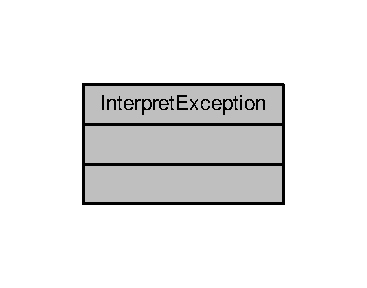
\includegraphics[width=176pt]{class_interpret_exception__coll__graph}
\end{center}
\end{figure}


\subsection{Detailed Description}
\begin{Desc}
\item[Examples\+: ]\par
\hyperlink{_2root_2_documents_2_git_clone_2_f_i_t__i_v_s__p_r_o_j_e_c_t2_2src_2_interpret_8h-example}{/root/\+Documents/\+Git\+Clone/\+F\+I\+T\+\_\+\+I\+V\+S\+\_\+\+P\+R\+O\+J\+E\+C\+T2/src/\+Interpret.\+h}.\end{Desc}


Definition at line 11 of file Interpret\+Exception.\+h.



The documentation for this class was generated from the following file\+:\begin{DoxyCompactItemize}
\item 
src/\hyperlink{_interpret_exception_8h}{Interpret\+Exception.\+h}\end{DoxyCompactItemize}

\hypertarget{classteam22_1_1_calc_1_1_lex}{}\section{team22\+:\+:Calc\+:\+:Lex Class Reference}
\label{classteam22_1_1_calc_1_1_lex}\index{team22\+::\+Calc\+::\+Lex@{team22\+::\+Calc\+::\+Lex}}


Reprezentace lexému kalkulačky tedy čísla nebo operace.  




{\ttfamily \#include $<$Lex.\+h$>$}



Collaboration diagram for team22\+:\+:Calc\+:\+:Lex\+:
\nopagebreak
\begin{figure}[H]
\begin{center}
\leavevmode
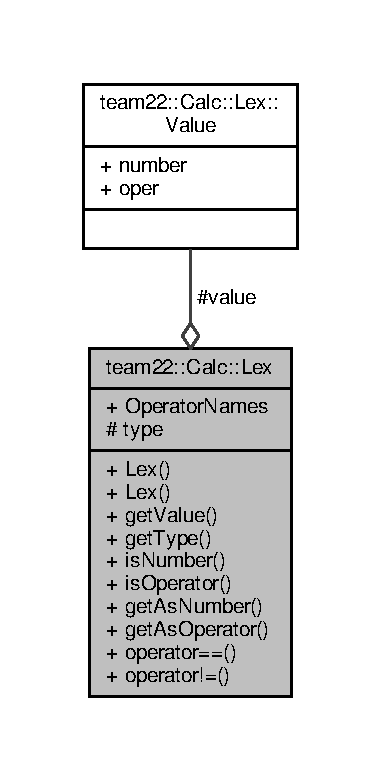
\includegraphics[height=550pt]{classteam22_1_1_calc_1_1_lex__coll__graph}
\end{center}
\end{figure}
\subsection*{Classes}
\begin{DoxyCompactItemize}
\item 
union \hyperlink{unionteam22_1_1_calc_1_1_lex_1_1_value}{Value}
\begin{DoxyCompactList}\small\item\em reprezentace hodnoty lexému \end{DoxyCompactList}\end{DoxyCompactItemize}
\subsection*{Public Types}
\begin{DoxyCompactItemize}
\item 
enum \hyperlink{classteam22_1_1_calc_1_1_lex_a295984577c98a23ddd20ee36d33145a2}{Types} \{ \hyperlink{classteam22_1_1_calc_1_1_lex_a295984577c98a23ddd20ee36d33145a2aa5609722e27933f9074b148e98c70a3b}{O\+P\+E\+R\+A\+T\+OR}, 
\hyperlink{classteam22_1_1_calc_1_1_lex_a295984577c98a23ddd20ee36d33145a2a016603184e8463620cf841dec9b33783}{N\+U\+M\+B\+ER}
 \}\begin{DoxyCompactList}\small\item\em Typy lexémů \end{DoxyCompactList}
\item 
enum \hyperlink{classteam22_1_1_calc_1_1_lex_a61d29fc4878a3b36d2de2f13c56ed932}{Operator} \{ \newline
\hyperlink{classteam22_1_1_calc_1_1_lex_a61d29fc4878a3b36d2de2f13c56ed932a8ea23c5d5cafb66151f94ce0fc7e3677}{A\+DD}, 
\hyperlink{classteam22_1_1_calc_1_1_lex_a61d29fc4878a3b36d2de2f13c56ed932a8fef3694ea5e14ff416907e90fb736c4}{S\+UB}, 
\hyperlink{classteam22_1_1_calc_1_1_lex_a61d29fc4878a3b36d2de2f13c56ed932adb91fbbc380e598b3d09bc424f799516}{D\+IV}, 
\hyperlink{classteam22_1_1_calc_1_1_lex_a61d29fc4878a3b36d2de2f13c56ed932a61a3bc185249f37b2a196b55f3b5a427}{M\+UL}, 
\newline
\hyperlink{classteam22_1_1_calc_1_1_lex_a61d29fc4878a3b36d2de2f13c56ed932ab68440fd94bc855e96432f0734dd6388}{E\+XP}, 
\hyperlink{classteam22_1_1_calc_1_1_lex_a61d29fc4878a3b36d2de2f13c56ed932ad9dc68a37981eff61741cbc660839f6f}{R\+O\+OT}, 
\hyperlink{classteam22_1_1_calc_1_1_lex_a61d29fc4878a3b36d2de2f13c56ed932a88420075287a73244fcaa4f2f851fc65}{F\+A\+C\+T\+O\+R\+I\+AL}, 
\hyperlink{classteam22_1_1_calc_1_1_lex_a61d29fc4878a3b36d2de2f13c56ed932a70d91e1bc184de6388bd44d6fd83e0da}{M\+OD}, 
\newline
\hyperlink{classteam22_1_1_calc_1_1_lex_a61d29fc4878a3b36d2de2f13c56ed932af8b2b375f8262ba1269fe245d7f19853}{N\+EG}, 
\hyperlink{classteam22_1_1_calc_1_1_lex_a61d29fc4878a3b36d2de2f13c56ed932a3c1443c79523cadf6582f238c04a015f}{E\+V\+AL}, 
\hyperlink{classteam22_1_1_calc_1_1_lex_a61d29fc4878a3b36d2de2f13c56ed932a4281d7ef6ac8dbf79c87603ca20c351c}{C\+L\+E\+AR}, 
\hyperlink{classteam22_1_1_calc_1_1_lex_a61d29fc4878a3b36d2de2f13c56ed932ac62fe9cff8a15f20fb1416612309ae80}{BS}
 \}\begin{DoxyCompactList}\small\item\em Jednotlivé operace. \end{DoxyCompactList}
\end{DoxyCompactItemize}
\subsection*{Public Member Functions}
\begin{DoxyCompactItemize}
\item 
\hyperlink{classteam22_1_1_calc_1_1_lex_a12b6acfadebf09ce47319315f8a2e684}{Lex} (\hyperlink{classteam22_1_1_calc_1_1_lex_a61d29fc4878a3b36d2de2f13c56ed932}{Operator} oper)
\begin{DoxyCompactList}\small\item\em Konstrukce lexému typu operátor. \end{DoxyCompactList}\item 
\hyperlink{classteam22_1_1_calc_1_1_lex_a95deefe4c4e987fef602fbd621bac095}{Lex} (\hyperlink{classteam22_1_1_math_1_1_number}{Math\+::\+Number} number)
\begin{DoxyCompactList}\small\item\em Konstrukce lexému typu číslo. \end{DoxyCompactList}\item 
const \hyperlink{unionteam22_1_1_calc_1_1_lex_1_1_value}{Value} \& \hyperlink{classteam22_1_1_calc_1_1_lex_a8a68cd13a68d32d50d3b014ca4478fab}{get\+Value} () const
\begin{DoxyCompactList}\small\item\em vrací hodnotu lexému \end{DoxyCompactList}\item 
\hyperlink{classteam22_1_1_calc_1_1_lex_a295984577c98a23ddd20ee36d33145a2}{Types} \hyperlink{classteam22_1_1_calc_1_1_lex_ae82ccde78beed14c45df1e747ed21bcb}{get\+Type} () const
\begin{DoxyCompactList}\small\item\em vrací typ lexému \end{DoxyCompactList}\item 
bool \hyperlink{classteam22_1_1_calc_1_1_lex_a21f9fe1956185bfb6d80d094846a44f1}{is\+Number} () const
\begin{DoxyCompactList}\small\item\em Testuje zda je lexém číslo. \end{DoxyCompactList}\item 
bool \hyperlink{classteam22_1_1_calc_1_1_lex_a965eff3f3264440279ea9a1f1d3a3cfe}{is\+Operator} () const
\begin{DoxyCompactList}\small\item\em Testuje zda je lexém operátor. \end{DoxyCompactList}\item 
\hyperlink{classteam22_1_1_math_1_1_number}{Math\+::\+Number} \hyperlink{classteam22_1_1_calc_1_1_lex_a794e75373451a906a2cfc60e5d6b1996}{get\+As\+Number} () const
\item 
\hyperlink{classteam22_1_1_calc_1_1_lex_a61d29fc4878a3b36d2de2f13c56ed932}{Operator} \hyperlink{classteam22_1_1_calc_1_1_lex_afdeee7e9b13fcb9826d4d8fd7d5f141f}{get\+As\+Operator} () const
\item 
bool \hyperlink{classteam22_1_1_calc_1_1_lex_a55858e2719cb121fccff59eed42dd692}{operator==} (const \hyperlink{classteam22_1_1_calc_1_1_lex}{Lex} \&rhs) const
\item 
bool \hyperlink{classteam22_1_1_calc_1_1_lex_a25b4f3b98b68c4d967eb3695efc78667}{operator!=} (const \hyperlink{classteam22_1_1_calc_1_1_lex}{Lex} \&rhs) const
\end{DoxyCompactItemize}
\subsection*{Public Attributes}
\begin{DoxyCompactItemize}
\item 
const char $\ast$ \hyperlink{classteam22_1_1_calc_1_1_lex_a9d280854466641dfb02159cc4afeec1f}{Operator\+Names} \mbox{[}12\mbox{]}
\begin{DoxyCompactList}\small\item\em A\+DD,. \end{DoxyCompactList}\end{DoxyCompactItemize}
\subsection*{Protected Attributes}
\begin{DoxyCompactItemize}
\item 
\hyperlink{unionteam22_1_1_calc_1_1_lex_1_1_value}{Value} \hyperlink{classteam22_1_1_calc_1_1_lex_a8a78a736b719931cada0905ac13fedc8}{value}
\item 
\hyperlink{classteam22_1_1_calc_1_1_lex_a295984577c98a23ddd20ee36d33145a2}{Types} \hyperlink{classteam22_1_1_calc_1_1_lex_a733fda9ebfa5ed6f588457d0870e81bc}{type}
\end{DoxyCompactItemize}
\subsection*{Friends}
\begin{DoxyCompactItemize}
\item 
std\+::ostream \& \hyperlink{classteam22_1_1_calc_1_1_lex_aca03505bafd6049109d56fd123d2dae6}{operator$<$$<$} (std\+::ostream \&os, const \hyperlink{classteam22_1_1_calc_1_1_lex}{Lex} \&lex)
\item 
std\+::stringstream \& \hyperlink{classteam22_1_1_calc_1_1_lex_a75f9b47ca9b4289a569608f62336b3dd}{operator$<$$<$} (std\+::stringstream \&os, const \hyperlink{classteam22_1_1_calc_1_1_lex}{Lex} \&lex)
\end{DoxyCompactItemize}


\subsection{Detailed Description}
Reprezentace lexému kalkulačky tedy čísla nebo operace. 

Definition at line 18 of file Lex.\+h.



\subsection{Member Enumeration Documentation}
\mbox{\Hypertarget{classteam22_1_1_calc_1_1_lex_a61d29fc4878a3b36d2de2f13c56ed932}\label{classteam22_1_1_calc_1_1_lex_a61d29fc4878a3b36d2de2f13c56ed932}} 
\index{team22\+::\+Calc\+::\+Lex@{team22\+::\+Calc\+::\+Lex}!Operator@{Operator}}
\index{Operator@{Operator}!team22\+::\+Calc\+::\+Lex@{team22\+::\+Calc\+::\+Lex}}
\subsubsection{\texorpdfstring{Operator}{Operator}}
{\footnotesize\ttfamily enum \hyperlink{classteam22_1_1_calc_1_1_lex_a61d29fc4878a3b36d2de2f13c56ed932}{team22\+::\+Calc\+::\+Lex\+::\+Operator}}



Jednotlivé operace. 

\begin{DoxyEnumFields}{Enumerator}
\raisebox{\heightof{T}}[0pt][0pt]{\index{A\+DD@{A\+DD}!team22\+::\+Calc\+::\+Lex@{team22\+::\+Calc\+::\+Lex}}\index{team22\+::\+Calc\+::\+Lex@{team22\+::\+Calc\+::\+Lex}!A\+DD@{A\+DD}}}\mbox{\Hypertarget{classteam22_1_1_calc_1_1_lex_a61d29fc4878a3b36d2de2f13c56ed932a8ea23c5d5cafb66151f94ce0fc7e3677}\label{classteam22_1_1_calc_1_1_lex_a61d29fc4878a3b36d2de2f13c56ed932a8ea23c5d5cafb66151f94ce0fc7e3677}} 
A\+DD&\\
\hline

\raisebox{\heightof{T}}[0pt][0pt]{\index{S\+UB@{S\+UB}!team22\+::\+Calc\+::\+Lex@{team22\+::\+Calc\+::\+Lex}}\index{team22\+::\+Calc\+::\+Lex@{team22\+::\+Calc\+::\+Lex}!S\+UB@{S\+UB}}}\mbox{\Hypertarget{classteam22_1_1_calc_1_1_lex_a61d29fc4878a3b36d2de2f13c56ed932a8fef3694ea5e14ff416907e90fb736c4}\label{classteam22_1_1_calc_1_1_lex_a61d29fc4878a3b36d2de2f13c56ed932a8fef3694ea5e14ff416907e90fb736c4}} 
S\+UB&\\
\hline

\raisebox{\heightof{T}}[0pt][0pt]{\index{D\+IV@{D\+IV}!team22\+::\+Calc\+::\+Lex@{team22\+::\+Calc\+::\+Lex}}\index{team22\+::\+Calc\+::\+Lex@{team22\+::\+Calc\+::\+Lex}!D\+IV@{D\+IV}}}\mbox{\Hypertarget{classteam22_1_1_calc_1_1_lex_a61d29fc4878a3b36d2de2f13c56ed932adb91fbbc380e598b3d09bc424f799516}\label{classteam22_1_1_calc_1_1_lex_a61d29fc4878a3b36d2de2f13c56ed932adb91fbbc380e598b3d09bc424f799516}} 
D\+IV&\\
\hline

\raisebox{\heightof{T}}[0pt][0pt]{\index{M\+UL@{M\+UL}!team22\+::\+Calc\+::\+Lex@{team22\+::\+Calc\+::\+Lex}}\index{team22\+::\+Calc\+::\+Lex@{team22\+::\+Calc\+::\+Lex}!M\+UL@{M\+UL}}}\mbox{\Hypertarget{classteam22_1_1_calc_1_1_lex_a61d29fc4878a3b36d2de2f13c56ed932a61a3bc185249f37b2a196b55f3b5a427}\label{classteam22_1_1_calc_1_1_lex_a61d29fc4878a3b36d2de2f13c56ed932a61a3bc185249f37b2a196b55f3b5a427}} 
M\+UL&\\
\hline

\raisebox{\heightof{T}}[0pt][0pt]{\index{E\+XP@{E\+XP}!team22\+::\+Calc\+::\+Lex@{team22\+::\+Calc\+::\+Lex}}\index{team22\+::\+Calc\+::\+Lex@{team22\+::\+Calc\+::\+Lex}!E\+XP@{E\+XP}}}\mbox{\Hypertarget{classteam22_1_1_calc_1_1_lex_a61d29fc4878a3b36d2de2f13c56ed932ab68440fd94bc855e96432f0734dd6388}\label{classteam22_1_1_calc_1_1_lex_a61d29fc4878a3b36d2de2f13c56ed932ab68440fd94bc855e96432f0734dd6388}} 
E\+XP&\\
\hline

\raisebox{\heightof{T}}[0pt][0pt]{\index{R\+O\+OT@{R\+O\+OT}!team22\+::\+Calc\+::\+Lex@{team22\+::\+Calc\+::\+Lex}}\index{team22\+::\+Calc\+::\+Lex@{team22\+::\+Calc\+::\+Lex}!R\+O\+OT@{R\+O\+OT}}}\mbox{\Hypertarget{classteam22_1_1_calc_1_1_lex_a61d29fc4878a3b36d2de2f13c56ed932ad9dc68a37981eff61741cbc660839f6f}\label{classteam22_1_1_calc_1_1_lex_a61d29fc4878a3b36d2de2f13c56ed932ad9dc68a37981eff61741cbc660839f6f}} 
R\+O\+OT&\\
\hline

\raisebox{\heightof{T}}[0pt][0pt]{\index{F\+A\+C\+T\+O\+R\+I\+AL@{F\+A\+C\+T\+O\+R\+I\+AL}!team22\+::\+Calc\+::\+Lex@{team22\+::\+Calc\+::\+Lex}}\index{team22\+::\+Calc\+::\+Lex@{team22\+::\+Calc\+::\+Lex}!F\+A\+C\+T\+O\+R\+I\+AL@{F\+A\+C\+T\+O\+R\+I\+AL}}}\mbox{\Hypertarget{classteam22_1_1_calc_1_1_lex_a61d29fc4878a3b36d2de2f13c56ed932a88420075287a73244fcaa4f2f851fc65}\label{classteam22_1_1_calc_1_1_lex_a61d29fc4878a3b36d2de2f13c56ed932a88420075287a73244fcaa4f2f851fc65}} 
F\+A\+C\+T\+O\+R\+I\+AL&\\
\hline

\raisebox{\heightof{T}}[0pt][0pt]{\index{M\+OD@{M\+OD}!team22\+::\+Calc\+::\+Lex@{team22\+::\+Calc\+::\+Lex}}\index{team22\+::\+Calc\+::\+Lex@{team22\+::\+Calc\+::\+Lex}!M\+OD@{M\+OD}}}\mbox{\Hypertarget{classteam22_1_1_calc_1_1_lex_a61d29fc4878a3b36d2de2f13c56ed932a70d91e1bc184de6388bd44d6fd83e0da}\label{classteam22_1_1_calc_1_1_lex_a61d29fc4878a3b36d2de2f13c56ed932a70d91e1bc184de6388bd44d6fd83e0da}} 
M\+OD&\\
\hline

\raisebox{\heightof{T}}[0pt][0pt]{\index{N\+EG@{N\+EG}!team22\+::\+Calc\+::\+Lex@{team22\+::\+Calc\+::\+Lex}}\index{team22\+::\+Calc\+::\+Lex@{team22\+::\+Calc\+::\+Lex}!N\+EG@{N\+EG}}}\mbox{\Hypertarget{classteam22_1_1_calc_1_1_lex_a61d29fc4878a3b36d2de2f13c56ed932af8b2b375f8262ba1269fe245d7f19853}\label{classteam22_1_1_calc_1_1_lex_a61d29fc4878a3b36d2de2f13c56ed932af8b2b375f8262ba1269fe245d7f19853}} 
N\+EG&\\
\hline

\raisebox{\heightof{T}}[0pt][0pt]{\index{E\+V\+AL@{E\+V\+AL}!team22\+::\+Calc\+::\+Lex@{team22\+::\+Calc\+::\+Lex}}\index{team22\+::\+Calc\+::\+Lex@{team22\+::\+Calc\+::\+Lex}!E\+V\+AL@{E\+V\+AL}}}\mbox{\Hypertarget{classteam22_1_1_calc_1_1_lex_a61d29fc4878a3b36d2de2f13c56ed932a3c1443c79523cadf6582f238c04a015f}\label{classteam22_1_1_calc_1_1_lex_a61d29fc4878a3b36d2de2f13c56ed932a3c1443c79523cadf6582f238c04a015f}} 
E\+V\+AL&\\
\hline

\raisebox{\heightof{T}}[0pt][0pt]{\index{C\+L\+E\+AR@{C\+L\+E\+AR}!team22\+::\+Calc\+::\+Lex@{team22\+::\+Calc\+::\+Lex}}\index{team22\+::\+Calc\+::\+Lex@{team22\+::\+Calc\+::\+Lex}!C\+L\+E\+AR@{C\+L\+E\+AR}}}\mbox{\Hypertarget{classteam22_1_1_calc_1_1_lex_a61d29fc4878a3b36d2de2f13c56ed932a4281d7ef6ac8dbf79c87603ca20c351c}\label{classteam22_1_1_calc_1_1_lex_a61d29fc4878a3b36d2de2f13c56ed932a4281d7ef6ac8dbf79c87603ca20c351c}} 
C\+L\+E\+AR&\\
\hline

\raisebox{\heightof{T}}[0pt][0pt]{\index{BS@{BS}!team22\+::\+Calc\+::\+Lex@{team22\+::\+Calc\+::\+Lex}}\index{team22\+::\+Calc\+::\+Lex@{team22\+::\+Calc\+::\+Lex}!BS@{BS}}}\mbox{\Hypertarget{classteam22_1_1_calc_1_1_lex_a61d29fc4878a3b36d2de2f13c56ed932ac62fe9cff8a15f20fb1416612309ae80}\label{classteam22_1_1_calc_1_1_lex_a61d29fc4878a3b36d2de2f13c56ed932ac62fe9cff8a15f20fb1416612309ae80}} 
BS&\\
\hline

\end{DoxyEnumFields}


Definition at line 33 of file Lex.\+h.

\mbox{\Hypertarget{classteam22_1_1_calc_1_1_lex_a295984577c98a23ddd20ee36d33145a2}\label{classteam22_1_1_calc_1_1_lex_a295984577c98a23ddd20ee36d33145a2}} 
\index{team22\+::\+Calc\+::\+Lex@{team22\+::\+Calc\+::\+Lex}!Types@{Types}}
\index{Types@{Types}!team22\+::\+Calc\+::\+Lex@{team22\+::\+Calc\+::\+Lex}}
\subsubsection{\texorpdfstring{Types}{Types}}
{\footnotesize\ttfamily enum \hyperlink{classteam22_1_1_calc_1_1_lex_a295984577c98a23ddd20ee36d33145a2}{team22\+::\+Calc\+::\+Lex\+::\+Types}}



Typy lexémů 

\begin{DoxyEnumFields}{Enumerator}
\raisebox{\heightof{T}}[0pt][0pt]{\index{O\+P\+E\+R\+A\+T\+OR@{O\+P\+E\+R\+A\+T\+OR}!team22\+::\+Calc\+::\+Lex@{team22\+::\+Calc\+::\+Lex}}\index{team22\+::\+Calc\+::\+Lex@{team22\+::\+Calc\+::\+Lex}!O\+P\+E\+R\+A\+T\+OR@{O\+P\+E\+R\+A\+T\+OR}}}\mbox{\Hypertarget{classteam22_1_1_calc_1_1_lex_a295984577c98a23ddd20ee36d33145a2aa5609722e27933f9074b148e98c70a3b}\label{classteam22_1_1_calc_1_1_lex_a295984577c98a23ddd20ee36d33145a2aa5609722e27933f9074b148e98c70a3b}} 
O\+P\+E\+R\+A\+T\+OR&\\
\hline

\raisebox{\heightof{T}}[0pt][0pt]{\index{N\+U\+M\+B\+ER@{N\+U\+M\+B\+ER}!team22\+::\+Calc\+::\+Lex@{team22\+::\+Calc\+::\+Lex}}\index{team22\+::\+Calc\+::\+Lex@{team22\+::\+Calc\+::\+Lex}!N\+U\+M\+B\+ER@{N\+U\+M\+B\+ER}}}\mbox{\Hypertarget{classteam22_1_1_calc_1_1_lex_a295984577c98a23ddd20ee36d33145a2a016603184e8463620cf841dec9b33783}\label{classteam22_1_1_calc_1_1_lex_a295984577c98a23ddd20ee36d33145a2a016603184e8463620cf841dec9b33783}} 
N\+U\+M\+B\+ER&\\
\hline

\end{DoxyEnumFields}


Definition at line 24 of file Lex.\+h.



\subsection{Constructor \& Destructor Documentation}
\mbox{\Hypertarget{classteam22_1_1_calc_1_1_lex_a12b6acfadebf09ce47319315f8a2e684}\label{classteam22_1_1_calc_1_1_lex_a12b6acfadebf09ce47319315f8a2e684}} 
\index{team22\+::\+Calc\+::\+Lex@{team22\+::\+Calc\+::\+Lex}!Lex@{Lex}}
\index{Lex@{Lex}!team22\+::\+Calc\+::\+Lex@{team22\+::\+Calc\+::\+Lex}}
\subsubsection{\texorpdfstring{Lex()}{Lex()}\hspace{0.1cm}{\footnotesize\ttfamily [1/2]}}
{\footnotesize\ttfamily team22\+::\+Calc\+::\+Lex\+::\+Lex (\begin{DoxyParamCaption}\item[{\hyperlink{classteam22_1_1_calc_1_1_lex_a61d29fc4878a3b36d2de2f13c56ed932}{Operator}}]{oper }\end{DoxyParamCaption})}



Konstrukce lexému typu operátor. 


\begin{DoxyParams}{Parameters}
{\em oper} & \\
\hline
\end{DoxyParams}


Definition at line 30 of file Lex.\+cpp.



References team22\+::\+Calc\+::\+Lex\+::\+Value\+::oper, and value.

\mbox{\Hypertarget{classteam22_1_1_calc_1_1_lex_a95deefe4c4e987fef602fbd621bac095}\label{classteam22_1_1_calc_1_1_lex_a95deefe4c4e987fef602fbd621bac095}} 
\index{team22\+::\+Calc\+::\+Lex@{team22\+::\+Calc\+::\+Lex}!Lex@{Lex}}
\index{Lex@{Lex}!team22\+::\+Calc\+::\+Lex@{team22\+::\+Calc\+::\+Lex}}
\subsubsection{\texorpdfstring{Lex()}{Lex()}\hspace{0.1cm}{\footnotesize\ttfamily [2/2]}}
{\footnotesize\ttfamily team22\+::\+Calc\+::\+Lex\+::\+Lex (\begin{DoxyParamCaption}\item[{\hyperlink{classteam22_1_1_math_1_1_number}{Math\+::\+Number}}]{number }\end{DoxyParamCaption})}



Konstrukce lexému typu číslo. 


\begin{DoxyParams}{Parameters}
{\em number} & \\
\hline
\end{DoxyParams}


Definition at line 36 of file Lex.\+cpp.



References team22\+::\+Calc\+::\+Lex\+::\+Value\+::number, and value.



\subsection{Member Function Documentation}
\mbox{\Hypertarget{classteam22_1_1_calc_1_1_lex_a794e75373451a906a2cfc60e5d6b1996}\label{classteam22_1_1_calc_1_1_lex_a794e75373451a906a2cfc60e5d6b1996}} 
\index{team22\+::\+Calc\+::\+Lex@{team22\+::\+Calc\+::\+Lex}!get\+As\+Number@{get\+As\+Number}}
\index{get\+As\+Number@{get\+As\+Number}!team22\+::\+Calc\+::\+Lex@{team22\+::\+Calc\+::\+Lex}}
\subsubsection{\texorpdfstring{get\+As\+Number()}{getAsNumber()}}
{\footnotesize\ttfamily \hyperlink{classteam22_1_1_math_1_1_number}{team22\+::\+Math\+::\+Number} team22\+::\+Calc\+::\+Lex\+::get\+As\+Number (\begin{DoxyParamCaption}{ }\end{DoxyParamCaption}) const}


\begin{DoxyExceptions}{Exceptions}
{\em \hyperlink{classteam22_1_1_calc_1_1_lex_exception}{Lex\+Exception}} & tento lexém pokud není číslo \\
\hline
\end{DoxyExceptions}
\begin{DoxyReturn}{Returns}
number 
\end{DoxyReturn}


Definition at line 42 of file Lex.\+cpp.



References is\+Number(), team22\+::\+Calc\+::\+Lex\+::\+Value\+::number, and value.



Referenced by operator!=(), and operator==().

\mbox{\Hypertarget{classteam22_1_1_calc_1_1_lex_afdeee7e9b13fcb9826d4d8fd7d5f141f}\label{classteam22_1_1_calc_1_1_lex_afdeee7e9b13fcb9826d4d8fd7d5f141f}} 
\index{team22\+::\+Calc\+::\+Lex@{team22\+::\+Calc\+::\+Lex}!get\+As\+Operator@{get\+As\+Operator}}
\index{get\+As\+Operator@{get\+As\+Operator}!team22\+::\+Calc\+::\+Lex@{team22\+::\+Calc\+::\+Lex}}
\subsubsection{\texorpdfstring{get\+As\+Operator()}{getAsOperator()}}
{\footnotesize\ttfamily \hyperlink{classteam22_1_1_calc_1_1_lex_a61d29fc4878a3b36d2de2f13c56ed932}{team22\+::\+Calc\+::\+Lex\+::\+Operator} team22\+::\+Calc\+::\+Lex\+::get\+As\+Operator (\begin{DoxyParamCaption}{ }\end{DoxyParamCaption}) const}


\begin{DoxyExceptions}{Exceptions}
{\em \hyperlink{classteam22_1_1_calc_1_1_lex_exception}{Lex\+Exception}} & tento lexém pokud není Operator \\
\hline
\end{DoxyExceptions}
\begin{DoxyReturn}{Returns}
operator 
\end{DoxyReturn}


Definition at line 50 of file Lex.\+cpp.



References is\+Operator(), team22\+::\+Calc\+::\+Lex\+::\+Value\+::oper, and value.



Referenced by operator!=(), operator==(), and team22\+::\+Calc\+::\+Equation\+::send\+Identified\+Lex().

\mbox{\Hypertarget{classteam22_1_1_calc_1_1_lex_ae82ccde78beed14c45df1e747ed21bcb}\label{classteam22_1_1_calc_1_1_lex_ae82ccde78beed14c45df1e747ed21bcb}} 
\index{team22\+::\+Calc\+::\+Lex@{team22\+::\+Calc\+::\+Lex}!get\+Type@{get\+Type}}
\index{get\+Type@{get\+Type}!team22\+::\+Calc\+::\+Lex@{team22\+::\+Calc\+::\+Lex}}
\subsubsection{\texorpdfstring{get\+Type()}{getType()}}
{\footnotesize\ttfamily \hyperlink{classteam22_1_1_calc_1_1_lex_a295984577c98a23ddd20ee36d33145a2}{team22\+::\+Calc\+::\+Lex\+::\+Types} team22\+::\+Calc\+::\+Lex\+::get\+Type (\begin{DoxyParamCaption}{ }\end{DoxyParamCaption}) const}



vrací typ lexému 

\begin{DoxyReturn}{Returns}
type 
\end{DoxyReturn}


Definition at line 15 of file Lex.\+cpp.



References type.

\mbox{\Hypertarget{classteam22_1_1_calc_1_1_lex_a8a68cd13a68d32d50d3b014ca4478fab}\label{classteam22_1_1_calc_1_1_lex_a8a68cd13a68d32d50d3b014ca4478fab}} 
\index{team22\+::\+Calc\+::\+Lex@{team22\+::\+Calc\+::\+Lex}!get\+Value@{get\+Value}}
\index{get\+Value@{get\+Value}!team22\+::\+Calc\+::\+Lex@{team22\+::\+Calc\+::\+Lex}}
\subsubsection{\texorpdfstring{get\+Value()}{getValue()}}
{\footnotesize\ttfamily const \hyperlink{unionteam22_1_1_calc_1_1_lex_1_1_value}{team22\+::\+Calc\+::\+Lex\+::\+Value} \& team22\+::\+Calc\+::\+Lex\+::get\+Value (\begin{DoxyParamCaption}{ }\end{DoxyParamCaption}) const}



vrací hodnotu lexému 



Definition at line 10 of file Lex.\+cpp.



References value.

\mbox{\Hypertarget{classteam22_1_1_calc_1_1_lex_a21f9fe1956185bfb6d80d094846a44f1}\label{classteam22_1_1_calc_1_1_lex_a21f9fe1956185bfb6d80d094846a44f1}} 
\index{team22\+::\+Calc\+::\+Lex@{team22\+::\+Calc\+::\+Lex}!is\+Number@{is\+Number}}
\index{is\+Number@{is\+Number}!team22\+::\+Calc\+::\+Lex@{team22\+::\+Calc\+::\+Lex}}
\subsubsection{\texorpdfstring{is\+Number()}{isNumber()}}
{\footnotesize\ttfamily bool team22\+::\+Calc\+::\+Lex\+::is\+Number (\begin{DoxyParamCaption}{ }\end{DoxyParamCaption}) const}



Testuje zda je lexém číslo. 

\begin{DoxyReturn}{Returns}
true pokud je číslo 
\end{DoxyReturn}


Definition at line 20 of file Lex.\+cpp.



References type.



Referenced by get\+As\+Number(), operator!=(), and operator==().

\mbox{\Hypertarget{classteam22_1_1_calc_1_1_lex_a965eff3f3264440279ea9a1f1d3a3cfe}\label{classteam22_1_1_calc_1_1_lex_a965eff3f3264440279ea9a1f1d3a3cfe}} 
\index{team22\+::\+Calc\+::\+Lex@{team22\+::\+Calc\+::\+Lex}!is\+Operator@{is\+Operator}}
\index{is\+Operator@{is\+Operator}!team22\+::\+Calc\+::\+Lex@{team22\+::\+Calc\+::\+Lex}}
\subsubsection{\texorpdfstring{is\+Operator()}{isOperator()}}
{\footnotesize\ttfamily bool team22\+::\+Calc\+::\+Lex\+::is\+Operator (\begin{DoxyParamCaption}{ }\end{DoxyParamCaption}) const}



Testuje zda je lexém operátor. 

\begin{DoxyReturn}{Returns}
true pokud je operátor 
\end{DoxyReturn}


Definition at line 25 of file Lex.\+cpp.



References type.



Referenced by get\+As\+Operator(), operator==(), and team22\+::\+Calc\+::\+Equation\+::send\+Identified\+Lex().

\mbox{\Hypertarget{classteam22_1_1_calc_1_1_lex_a25b4f3b98b68c4d967eb3695efc78667}\label{classteam22_1_1_calc_1_1_lex_a25b4f3b98b68c4d967eb3695efc78667}} 
\index{team22\+::\+Calc\+::\+Lex@{team22\+::\+Calc\+::\+Lex}!operator"!=@{operator"!=}}
\index{operator"!=@{operator"!=}!team22\+::\+Calc\+::\+Lex@{team22\+::\+Calc\+::\+Lex}}
\subsubsection{\texorpdfstring{operator"!=()}{operator!=()}}
{\footnotesize\ttfamily bool team22\+::\+Calc\+::\+Lex\+::operator!= (\begin{DoxyParamCaption}\item[{const \hyperlink{classteam22_1_1_calc_1_1_lex}{Lex} \&}]{rhs }\end{DoxyParamCaption}) const}



Definition at line 69 of file Lex.\+cpp.



References get\+As\+Number(), get\+As\+Operator(), is\+Number(), and Operator\+Names.

\mbox{\Hypertarget{classteam22_1_1_calc_1_1_lex_a55858e2719cb121fccff59eed42dd692}\label{classteam22_1_1_calc_1_1_lex_a55858e2719cb121fccff59eed42dd692}} 
\index{team22\+::\+Calc\+::\+Lex@{team22\+::\+Calc\+::\+Lex}!operator==@{operator==}}
\index{operator==@{operator==}!team22\+::\+Calc\+::\+Lex@{team22\+::\+Calc\+::\+Lex}}
\subsubsection{\texorpdfstring{operator==()}{operator==()}}
{\footnotesize\ttfamily bool team22\+::\+Calc\+::\+Lex\+::operator== (\begin{DoxyParamCaption}\item[{const \hyperlink{classteam22_1_1_calc_1_1_lex}{Lex} \&}]{rhs }\end{DoxyParamCaption}) const}



Definition at line 59 of file Lex.\+cpp.



References get\+As\+Number(), get\+As\+Operator(), is\+Number(), is\+Operator(), and type.



\subsection{Friends And Related Function Documentation}
\mbox{\Hypertarget{classteam22_1_1_calc_1_1_lex_aca03505bafd6049109d56fd123d2dae6}\label{classteam22_1_1_calc_1_1_lex_aca03505bafd6049109d56fd123d2dae6}} 
\index{team22\+::\+Calc\+::\+Lex@{team22\+::\+Calc\+::\+Lex}!operator$<$$<$@{operator$<$$<$}}
\index{operator$<$$<$@{operator$<$$<$}!team22\+::\+Calc\+::\+Lex@{team22\+::\+Calc\+::\+Lex}}
\subsubsection{\texorpdfstring{operator$<$$<$}{operator<<}\hspace{0.1cm}{\footnotesize\ttfamily [1/2]}}
{\footnotesize\ttfamily std\+::ostream\& operator$<$$<$ (\begin{DoxyParamCaption}\item[{std\+::ostream \&}]{os,  }\item[{const \hyperlink{classteam22_1_1_calc_1_1_lex}{Lex} \&}]{lex }\end{DoxyParamCaption})\hspace{0.3cm}{\ttfamily [friend]}}

\mbox{\Hypertarget{classteam22_1_1_calc_1_1_lex_a75f9b47ca9b4289a569608f62336b3dd}\label{classteam22_1_1_calc_1_1_lex_a75f9b47ca9b4289a569608f62336b3dd}} 
\index{team22\+::\+Calc\+::\+Lex@{team22\+::\+Calc\+::\+Lex}!operator$<$$<$@{operator$<$$<$}}
\index{operator$<$$<$@{operator$<$$<$}!team22\+::\+Calc\+::\+Lex@{team22\+::\+Calc\+::\+Lex}}
\subsubsection{\texorpdfstring{operator$<$$<$}{operator<<}\hspace{0.1cm}{\footnotesize\ttfamily [2/2]}}
{\footnotesize\ttfamily std\+::stringstream\& operator$<$$<$ (\begin{DoxyParamCaption}\item[{std\+::stringstream \&}]{os,  }\item[{const \hyperlink{classteam22_1_1_calc_1_1_lex}{Lex} \&}]{lex }\end{DoxyParamCaption})\hspace{0.3cm}{\ttfamily [friend]}}



\subsection{Member Data Documentation}
\mbox{\Hypertarget{classteam22_1_1_calc_1_1_lex_a9d280854466641dfb02159cc4afeec1f}\label{classteam22_1_1_calc_1_1_lex_a9d280854466641dfb02159cc4afeec1f}} 
\index{team22\+::\+Calc\+::\+Lex@{team22\+::\+Calc\+::\+Lex}!Operator\+Names@{Operator\+Names}}
\index{Operator\+Names@{Operator\+Names}!team22\+::\+Calc\+::\+Lex@{team22\+::\+Calc\+::\+Lex}}
\subsubsection{\texorpdfstring{Operator\+Names}{OperatorNames}}
{\footnotesize\ttfamily const char$\ast$ team22\+::\+Calc\+::\+Lex\+::\+Operator\+Names\mbox{[}12\mbox{]}}

{\bfseries Initial value\+:}
\begin{DoxyCode}
\{
        \textcolor{stringliteral}{"+"},
        \textcolor{stringliteral}{"-"},
        \textcolor{stringliteral}{"/"},
        \textcolor{stringliteral}{"*"},
        \textcolor{stringliteral}{"^"},
        \textcolor{stringliteral}{"√"},
        \textcolor{stringliteral}{"!"},
        \textcolor{stringliteral}{"%"},
        \textcolor{stringliteral}{"*-1"},
        \textcolor{stringliteral}{"="},
        \textcolor{stringliteral}{"CLEAR"},
        \textcolor{stringliteral}{"BS"},
    \}
\end{DoxyCode}


A\+DD,. 

S\+UB, D\+IV, M\+UL, E\+XP, R\+O\+OT, F\+A\+C\+T\+O\+R\+I\+AL, M\+OD, N\+EG, E\+V\+AL, C\+L\+E\+AR, BS 

Definition at line 49 of file Lex.\+h.



Referenced by operator!=().

\mbox{\Hypertarget{classteam22_1_1_calc_1_1_lex_a733fda9ebfa5ed6f588457d0870e81bc}\label{classteam22_1_1_calc_1_1_lex_a733fda9ebfa5ed6f588457d0870e81bc}} 
\index{team22\+::\+Calc\+::\+Lex@{team22\+::\+Calc\+::\+Lex}!type@{type}}
\index{type@{type}!team22\+::\+Calc\+::\+Lex@{team22\+::\+Calc\+::\+Lex}}
\subsubsection{\texorpdfstring{type}{type}}
{\footnotesize\ttfamily \hyperlink{classteam22_1_1_calc_1_1_lex_a295984577c98a23ddd20ee36d33145a2}{Types} team22\+::\+Calc\+::\+Lex\+::type\hspace{0.3cm}{\ttfamily [protected]}}



Definition at line 75 of file Lex.\+h.



Referenced by get\+Type(), is\+Number(), is\+Operator(), and operator==().

\mbox{\Hypertarget{classteam22_1_1_calc_1_1_lex_a8a78a736b719931cada0905ac13fedc8}\label{classteam22_1_1_calc_1_1_lex_a8a78a736b719931cada0905ac13fedc8}} 
\index{team22\+::\+Calc\+::\+Lex@{team22\+::\+Calc\+::\+Lex}!value@{value}}
\index{value@{value}!team22\+::\+Calc\+::\+Lex@{team22\+::\+Calc\+::\+Lex}}
\subsubsection{\texorpdfstring{value}{value}}
{\footnotesize\ttfamily \hyperlink{unionteam22_1_1_calc_1_1_lex_1_1_value}{Value} team22\+::\+Calc\+::\+Lex\+::value\hspace{0.3cm}{\ttfamily [protected]}}



Definition at line 74 of file Lex.\+h.



Referenced by get\+As\+Number(), get\+As\+Operator(), get\+Value(), and Lex().



The documentation for this class was generated from the following files\+:\begin{DoxyCompactItemize}
\item 
src/\hyperlink{_lex_8h}{Lex.\+h}\item 
src/\hyperlink{_lex_8cpp}{Lex.\+cpp}\end{DoxyCompactItemize}

\hypertarget{classteam22_1_1_calc_1_1_lex_exception}{}\section{team22\+:\+:Calc\+:\+:Lex\+Exception Class Reference}
\label{classteam22_1_1_calc_1_1_lex_exception}\index{team22\+::\+Calc\+::\+Lex\+Exception@{team22\+::\+Calc\+::\+Lex\+Exception}}


{\ttfamily \#include $<$Lex\+Exception.\+h$>$}



Inheritance diagram for team22\+:\+:Calc\+:\+:Lex\+Exception\+:
\nopagebreak
\begin{figure}[H]
\begin{center}
\leavevmode
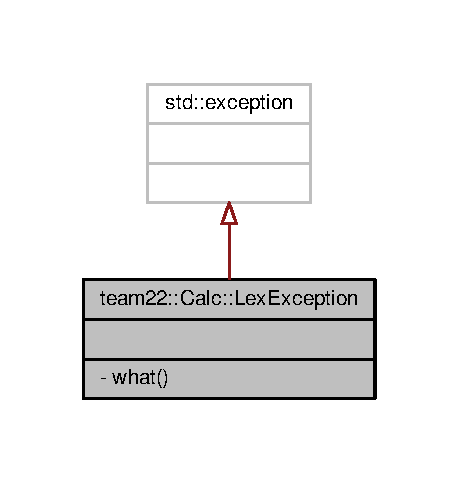
\includegraphics[width=220pt]{classteam22_1_1_calc_1_1_lex_exception__inherit__graph}
\end{center}
\end{figure}


Collaboration diagram for team22\+:\+:Calc\+:\+:Lex\+Exception\+:
\nopagebreak
\begin{figure}[H]
\begin{center}
\leavevmode
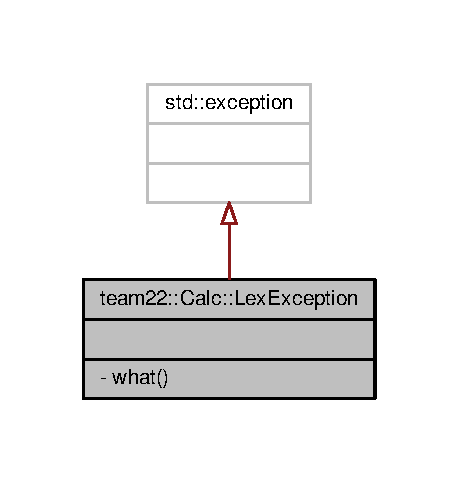
\includegraphics[width=220pt]{classteam22_1_1_calc_1_1_lex_exception__coll__graph}
\end{center}
\end{figure}
\subsection*{Private Member Functions}
\begin{DoxyCompactItemize}
\item 
const char $\ast$ \hyperlink{classteam22_1_1_calc_1_1_lex_exception_afeba1f355eee4aacad8cb7409b1ee3ea}{what} () const noexcept override
\end{DoxyCompactItemize}


\subsection{Detailed Description}
Víjymka pro Lexikální analyzátor 

Definition at line 18 of file Lex\+Exception.\+h.



\subsection{Member Function Documentation}
\mbox{\Hypertarget{classteam22_1_1_calc_1_1_lex_exception_afeba1f355eee4aacad8cb7409b1ee3ea}\label{classteam22_1_1_calc_1_1_lex_exception_afeba1f355eee4aacad8cb7409b1ee3ea}} 
\index{team22\+::\+Calc\+::\+Lex\+Exception@{team22\+::\+Calc\+::\+Lex\+Exception}!what@{what}}
\index{what@{what}!team22\+::\+Calc\+::\+Lex\+Exception@{team22\+::\+Calc\+::\+Lex\+Exception}}
\subsubsection{\texorpdfstring{what()}{what()}}
{\footnotesize\ttfamily const char$\ast$ team22\+::\+Calc\+::\+Lex\+Exception\+::what (\begin{DoxyParamCaption}{ }\end{DoxyParamCaption}) const\hspace{0.3cm}{\ttfamily [inline]}, {\ttfamily [override]}, {\ttfamily [private]}, {\ttfamily [noexcept]}}



Definition at line 23 of file Lex\+Exception.\+h.



The documentation for this class was generated from the following file\+:\begin{DoxyCompactItemize}
\item 
src/\hyperlink{_lex_exception_8h}{Lex\+Exception.\+h}\end{DoxyCompactItemize}

\hypertarget{classteam22_1_1_calc_1_1_lexical_analyzer}{}\section{team22\+:\+:Calc\+:\+:Lexical\+Analyzer Class Reference}
\label{classteam22_1_1_calc_1_1_lexical_analyzer}\index{team22\+::\+Calc\+::\+Lexical\+Analyzer@{team22\+::\+Calc\+::\+Lexical\+Analyzer}}


{\ttfamily \#include $<$Lexical\+Analyzer.\+h$>$}



Collaboration diagram for team22\+:\+:Calc\+:\+:Lexical\+Analyzer\+:
\nopagebreak
\begin{figure}[H]
\begin{center}
\leavevmode
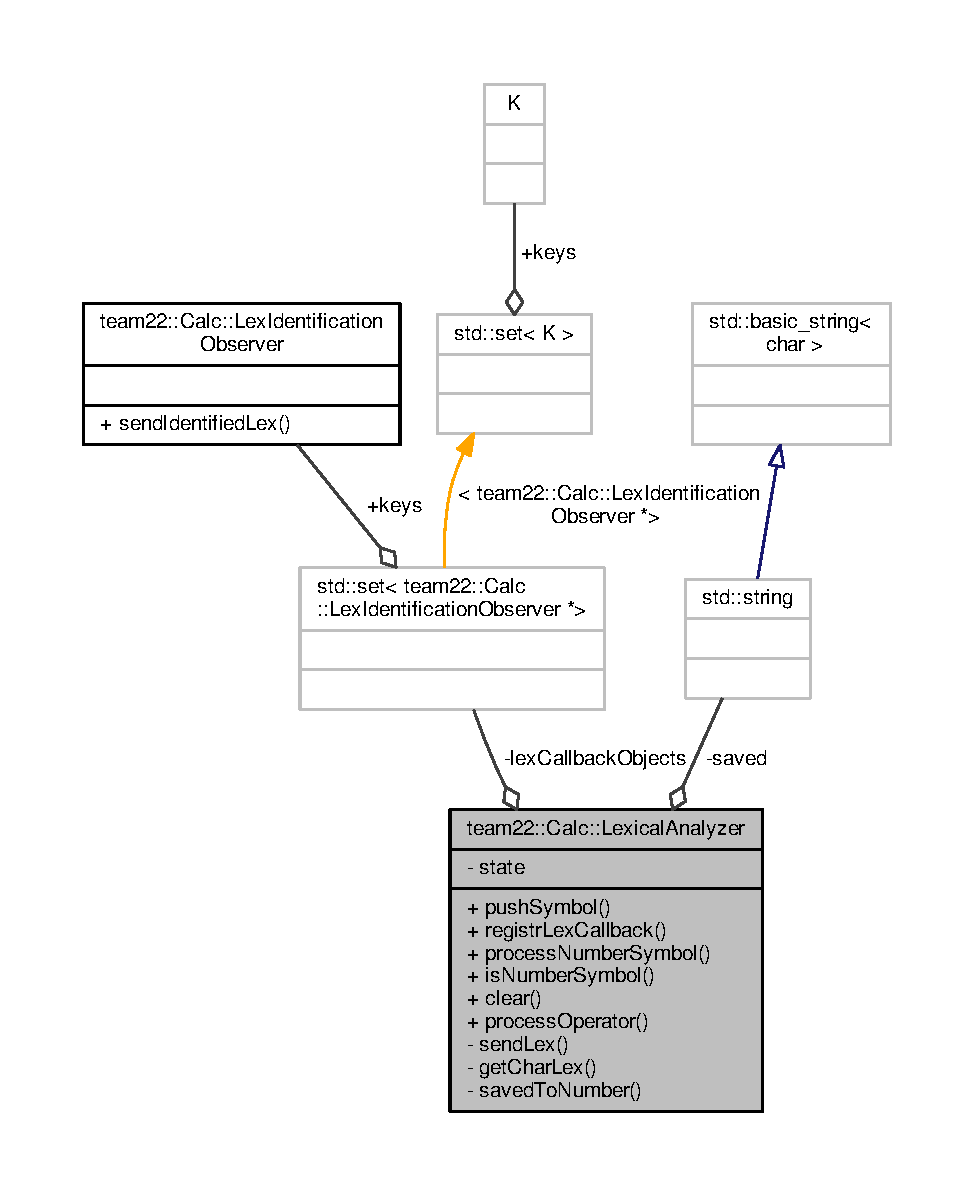
\includegraphics[width=350pt]{classteam22_1_1_calc_1_1_lexical_analyzer__coll__graph}
\end{center}
\end{figure}
\subsection*{Public Member Functions}
\begin{DoxyCompactItemize}
\item 
void \hyperlink{classteam22_1_1_calc_1_1_lexical_analyzer_af56c536f78c680bd635ac1173e65b492}{push\+Symbol} (char symbol)
\item 
void \hyperlink{classteam22_1_1_calc_1_1_lexical_analyzer_ae7fb3f4ce9e6020215352c0c9e2b8245}{registr\+Lex\+Callback} (\hyperlink{classteam22_1_1_calc_1_1_lex_identification_observer}{Lex\+Identification\+Observer} $\ast$lex\+Callback\+Object)
\item 
void \hyperlink{classteam22_1_1_calc_1_1_lexical_analyzer_a18ba04d046da0b11eec66fb2689ddfef}{process\+Number\+Symbol} (char symbol)
\item 
bool \hyperlink{classteam22_1_1_calc_1_1_lexical_analyzer_a922bf14131d064fce52bf126e8d29839}{is\+Number\+Symbol} (char symbol) const
\item 
void \hyperlink{classteam22_1_1_calc_1_1_lexical_analyzer_adf38772b29f998549aa532e8f380b4b2}{clear} ()
\item 
void \hyperlink{classteam22_1_1_calc_1_1_lexical_analyzer_ab84b6b8f52056452cd52b8abdb9a3faa}{process\+Operator} (char symbol)
\end{DoxyCompactItemize}
\subsection*{Private Types}
\begin{DoxyCompactItemize}
\item 
enum \hyperlink{classteam22_1_1_calc_1_1_lexical_analyzer_aef11ba66454715a80d5964c07f6d8cc3}{State} \{ \hyperlink{classteam22_1_1_calc_1_1_lexical_analyzer_aef11ba66454715a80d5964c07f6d8cc3a862f179df5de529676972b3b95c52f86}{Number}, 
\hyperlink{classteam22_1_1_calc_1_1_lexical_analyzer_aef11ba66454715a80d5964c07f6d8cc3ae2510b92e28892c94126aa4273470f78}{Operator}, 
\hyperlink{classteam22_1_1_calc_1_1_lexical_analyzer_aef11ba66454715a80d5964c07f6d8cc3a11976214c837f23fd71b2af8b0de3d5b}{Init}
 \}
\end{DoxyCompactItemize}
\subsection*{Private Member Functions}
\begin{DoxyCompactItemize}
\item 
void \hyperlink{classteam22_1_1_calc_1_1_lexical_analyzer_afd6bb48e5de7f8490addc9b326bfeb49}{send\+Lex} (\hyperlink{classteam22_1_1_calc_1_1_lex}{Lex} lex)
\item 
\hyperlink{classteam22_1_1_calc_1_1_lex}{Lex} \hyperlink{classteam22_1_1_calc_1_1_lexical_analyzer_a451aa3e3ed6f150d5b24fae76cc93cb4}{get\+Char\+Lex} (char \hyperlink{_number_8cpp_a3a6c194a55c239306d07bbf83f5972e9}{c})
\item 
\hyperlink{classteam22_1_1_math_1_1_number}{Math\+::\+Number} \hyperlink{classteam22_1_1_calc_1_1_lexical_analyzer_a689b52c49cd7c9e87dd468987472af83}{saved\+To\+Number} ()
\end{DoxyCompactItemize}
\subsection*{Private Attributes}
\begin{DoxyCompactItemize}
\item 
\hyperlink{classteam22_1_1_calc_1_1_lexical_analyzer_aef11ba66454715a80d5964c07f6d8cc3}{State} \hyperlink{classteam22_1_1_calc_1_1_lexical_analyzer_ad0f4710b09bf91a00d11846a7ef036ab}{state} = \hyperlink{classteam22_1_1_calc_1_1_lexical_analyzer_aef11ba66454715a80d5964c07f6d8cc3a11976214c837f23fd71b2af8b0de3d5b}{Init}
\item 
std\+::set$<$ \hyperlink{classteam22_1_1_calc_1_1_lex_identification_observer}{Lex\+Identification\+Observer} $\ast$ $>$ \hyperlink{classteam22_1_1_calc_1_1_lexical_analyzer_ab8018dc24a6f4e188a901c83bbd9fdb1}{lex\+Callback\+Objects}
\item 
std\+::string \hyperlink{classteam22_1_1_calc_1_1_lexical_analyzer_afd063de2c3d792b5688c863eb5135968}{saved} = \char`\"{}\char`\"{}
\end{DoxyCompactItemize}


\subsection{Detailed Description}
Třída sloužící k lexikální analyze vstupů přebírá znaky pomocí fce \hyperlink{classteam22_1_1_calc_1_1_lexical_analyzer_af56c536f78c680bd635ac1173e65b492}{push\+Symbol()} a ve chvíli identifikace lexému předá tento interpretu a pokud byl registrovaný volá callback kterému tento lexém předá. 

Definition at line 26 of file Lexical\+Analyzer.\+h.



\subsection{Member Enumeration Documentation}
\mbox{\Hypertarget{classteam22_1_1_calc_1_1_lexical_analyzer_aef11ba66454715a80d5964c07f6d8cc3}\label{classteam22_1_1_calc_1_1_lexical_analyzer_aef11ba66454715a80d5964c07f6d8cc3}} 
\index{team22\+::\+Calc\+::\+Lexical\+Analyzer@{team22\+::\+Calc\+::\+Lexical\+Analyzer}!State@{State}}
\index{State@{State}!team22\+::\+Calc\+::\+Lexical\+Analyzer@{team22\+::\+Calc\+::\+Lexical\+Analyzer}}
\subsubsection{\texorpdfstring{State}{State}}
{\footnotesize\ttfamily enum \hyperlink{classteam22_1_1_calc_1_1_lexical_analyzer_aef11ba66454715a80d5964c07f6d8cc3}{team22\+::\+Calc\+::\+Lexical\+Analyzer\+::\+State}\hspace{0.3cm}{\ttfamily [private]}}

\begin{DoxyEnumFields}{Enumerator}
\raisebox{\heightof{T}}[0pt][0pt]{\index{Number@{Number}!team22\+::\+Calc\+::\+Lexical\+Analyzer@{team22\+::\+Calc\+::\+Lexical\+Analyzer}}\index{team22\+::\+Calc\+::\+Lexical\+Analyzer@{team22\+::\+Calc\+::\+Lexical\+Analyzer}!Number@{Number}}}\mbox{\Hypertarget{classteam22_1_1_calc_1_1_lexical_analyzer_aef11ba66454715a80d5964c07f6d8cc3a862f179df5de529676972b3b95c52f86}\label{classteam22_1_1_calc_1_1_lexical_analyzer_aef11ba66454715a80d5964c07f6d8cc3a862f179df5de529676972b3b95c52f86}} 
Number&\\
\hline

\raisebox{\heightof{T}}[0pt][0pt]{\index{Operator@{Operator}!team22\+::\+Calc\+::\+Lexical\+Analyzer@{team22\+::\+Calc\+::\+Lexical\+Analyzer}}\index{team22\+::\+Calc\+::\+Lexical\+Analyzer@{team22\+::\+Calc\+::\+Lexical\+Analyzer}!Operator@{Operator}}}\mbox{\Hypertarget{classteam22_1_1_calc_1_1_lexical_analyzer_aef11ba66454715a80d5964c07f6d8cc3ae2510b92e28892c94126aa4273470f78}\label{classteam22_1_1_calc_1_1_lexical_analyzer_aef11ba66454715a80d5964c07f6d8cc3ae2510b92e28892c94126aa4273470f78}} 
Operator&\\
\hline

\raisebox{\heightof{T}}[0pt][0pt]{\index{Init@{Init}!team22\+::\+Calc\+::\+Lexical\+Analyzer@{team22\+::\+Calc\+::\+Lexical\+Analyzer}}\index{team22\+::\+Calc\+::\+Lexical\+Analyzer@{team22\+::\+Calc\+::\+Lexical\+Analyzer}!Init@{Init}}}\mbox{\Hypertarget{classteam22_1_1_calc_1_1_lexical_analyzer_aef11ba66454715a80d5964c07f6d8cc3a11976214c837f23fd71b2af8b0de3d5b}\label{classteam22_1_1_calc_1_1_lexical_analyzer_aef11ba66454715a80d5964c07f6d8cc3a11976214c837f23fd71b2af8b0de3d5b}} 
Init&\\
\hline

\end{DoxyEnumFields}


Definition at line 28 of file Lexical\+Analyzer.\+h.



\subsection{Member Function Documentation}
\mbox{\Hypertarget{classteam22_1_1_calc_1_1_lexical_analyzer_adf38772b29f998549aa532e8f380b4b2}\label{classteam22_1_1_calc_1_1_lexical_analyzer_adf38772b29f998549aa532e8f380b4b2}} 
\index{team22\+::\+Calc\+::\+Lexical\+Analyzer@{team22\+::\+Calc\+::\+Lexical\+Analyzer}!clear@{clear}}
\index{clear@{clear}!team22\+::\+Calc\+::\+Lexical\+Analyzer@{team22\+::\+Calc\+::\+Lexical\+Analyzer}}
\subsubsection{\texorpdfstring{clear()}{clear()}}
{\footnotesize\ttfamily void team22\+::\+Calc\+::\+Lexical\+Analyzer\+::clear (\begin{DoxyParamCaption}{ }\end{DoxyParamCaption})}

Vyresetuje lexikální analyzátor 

Definition at line 167 of file Lexical\+Analyzer.\+cpp.



References Init, saved, and state.



Referenced by process\+Number\+Symbol(), process\+Operator(), and push\+Symbol().

\mbox{\Hypertarget{classteam22_1_1_calc_1_1_lexical_analyzer_a451aa3e3ed6f150d5b24fae76cc93cb4}\label{classteam22_1_1_calc_1_1_lexical_analyzer_a451aa3e3ed6f150d5b24fae76cc93cb4}} 
\index{team22\+::\+Calc\+::\+Lexical\+Analyzer@{team22\+::\+Calc\+::\+Lexical\+Analyzer}!get\+Char\+Lex@{get\+Char\+Lex}}
\index{get\+Char\+Lex@{get\+Char\+Lex}!team22\+::\+Calc\+::\+Lexical\+Analyzer@{team22\+::\+Calc\+::\+Lexical\+Analyzer}}
\subsubsection{\texorpdfstring{get\+Char\+Lex()}{getCharLex()}}
{\footnotesize\ttfamily \hyperlink{classteam22_1_1_calc_1_1_lex}{Lex} team22\+::\+Calc\+::\+Lexical\+Analyzer\+::get\+Char\+Lex (\begin{DoxyParamCaption}\item[{char}]{c }\end{DoxyParamCaption})\hspace{0.3cm}{\ttfamily [private]}}

Vrací lexém daného znaku 
\begin{DoxyParams}{Parameters}
{\em c} & znak nebo číslice k převodu na lexém \\
\hline
\end{DoxyParams}


Definition at line 19 of file Lexical\+Analyzer.\+cpp.



References team22\+::\+Calc\+::\+Lex\+::\+A\+DD, team22\+::\+Calc\+::\+Lex\+::\+C\+L\+E\+AR, team22\+::\+Calc\+::\+Lex\+::\+D\+IV, team22\+::\+Calc\+::\+Lex\+::\+E\+V\+AL, team22\+::\+Calc\+::\+Lex\+::\+E\+XP, team22\+::\+Calc\+::\+Lex\+::\+F\+A\+C\+T\+O\+R\+I\+AL, team22\+::\+Calc\+::\+Lex\+::\+M\+OD, team22\+::\+Calc\+::\+Lex\+::\+M\+UL, and team22\+::\+Calc\+::\+Lex\+::\+S\+UB.



Referenced by push\+Symbol().

\mbox{\Hypertarget{classteam22_1_1_calc_1_1_lexical_analyzer_a922bf14131d064fce52bf126e8d29839}\label{classteam22_1_1_calc_1_1_lexical_analyzer_a922bf14131d064fce52bf126e8d29839}} 
\index{team22\+::\+Calc\+::\+Lexical\+Analyzer@{team22\+::\+Calc\+::\+Lexical\+Analyzer}!is\+Number\+Symbol@{is\+Number\+Symbol}}
\index{is\+Number\+Symbol@{is\+Number\+Symbol}!team22\+::\+Calc\+::\+Lexical\+Analyzer@{team22\+::\+Calc\+::\+Lexical\+Analyzer}}
\subsubsection{\texorpdfstring{is\+Number\+Symbol()}{isNumberSymbol()}}
{\footnotesize\ttfamily bool team22\+::\+Calc\+::\+Lexical\+Analyzer\+::is\+Number\+Symbol (\begin{DoxyParamCaption}\item[{char}]{symbol }\end{DoxyParamCaption}) const}

Jedná se o symbol tvořící číslo tedy číslice, . nebo i 
\begin{DoxyParams}{Parameters}
{\em symbol} & \\
\hline
\end{DoxyParams}
\begin{DoxyReturn}{Returns}

\end{DoxyReturn}


Definition at line 138 of file Lexical\+Analyzer.\+cpp.



Referenced by push\+Symbol().

\mbox{\Hypertarget{classteam22_1_1_calc_1_1_lexical_analyzer_a18ba04d046da0b11eec66fb2689ddfef}\label{classteam22_1_1_calc_1_1_lexical_analyzer_a18ba04d046da0b11eec66fb2689ddfef}} 
\index{team22\+::\+Calc\+::\+Lexical\+Analyzer@{team22\+::\+Calc\+::\+Lexical\+Analyzer}!process\+Number\+Symbol@{process\+Number\+Symbol}}
\index{process\+Number\+Symbol@{process\+Number\+Symbol}!team22\+::\+Calc\+::\+Lexical\+Analyzer@{team22\+::\+Calc\+::\+Lexical\+Analyzer}}
\subsubsection{\texorpdfstring{process\+Number\+Symbol()}{processNumberSymbol()}}
{\footnotesize\ttfamily void team22\+::\+Calc\+::\+Lexical\+Analyzer\+::process\+Number\+Symbol (\begin{DoxyParamCaption}\item[{char}]{symbol }\end{DoxyParamCaption})}

Zpracuje uložený řetězec saved a vrátí jej jako číslo 
\begin{DoxyParams}{Parameters}
{\em symbol} & \\
\hline
\end{DoxyParams}


Definition at line 148 of file Lexical\+Analyzer.\+cpp.



References clear(), Init, Number, saved, saved\+To\+Number(), send\+Lex(), and state.



Referenced by push\+Symbol().

\mbox{\Hypertarget{classteam22_1_1_calc_1_1_lexical_analyzer_ab84b6b8f52056452cd52b8abdb9a3faa}\label{classteam22_1_1_calc_1_1_lexical_analyzer_ab84b6b8f52056452cd52b8abdb9a3faa}} 
\index{team22\+::\+Calc\+::\+Lexical\+Analyzer@{team22\+::\+Calc\+::\+Lexical\+Analyzer}!process\+Operator@{process\+Operator}}
\index{process\+Operator@{process\+Operator}!team22\+::\+Calc\+::\+Lexical\+Analyzer@{team22\+::\+Calc\+::\+Lexical\+Analyzer}}
\subsubsection{\texorpdfstring{process\+Operator()}{processOperator()}}
{\footnotesize\ttfamily void team22\+::\+Calc\+::\+Lexical\+Analyzer\+::process\+Operator (\begin{DoxyParamCaption}\item[{char}]{symbol }\end{DoxyParamCaption})}

Zpracuje výceznakový operátor 
\begin{DoxyParams}{Parameters}
{\em symbol} & \\
\hline
\end{DoxyParams}


Definition at line 80 of file Lexical\+Analyzer.\+cpp.



References team22\+::\+Calc\+::\+Lex\+::\+BS, clear(), team22\+::\+Calc\+::\+Lex\+::\+N\+EG, Operator, team22\+::\+Calc\+::\+Lex\+::\+R\+O\+OT, saved, send\+Lex(), and state.



Referenced by push\+Symbol().

\mbox{\Hypertarget{classteam22_1_1_calc_1_1_lexical_analyzer_af56c536f78c680bd635ac1173e65b492}\label{classteam22_1_1_calc_1_1_lexical_analyzer_af56c536f78c680bd635ac1173e65b492}} 
\index{team22\+::\+Calc\+::\+Lexical\+Analyzer@{team22\+::\+Calc\+::\+Lexical\+Analyzer}!push\+Symbol@{push\+Symbol}}
\index{push\+Symbol@{push\+Symbol}!team22\+::\+Calc\+::\+Lexical\+Analyzer@{team22\+::\+Calc\+::\+Lexical\+Analyzer}}
\subsubsection{\texorpdfstring{push\+Symbol()}{pushSymbol()}}
{\footnotesize\ttfamily void team22\+::\+Calc\+::\+Lexical\+Analyzer\+::push\+Symbol (\begin{DoxyParamCaption}\item[{char}]{symbol }\end{DoxyParamCaption})}

Předá znak k analýze 
\begin{DoxyParams}{Parameters}
{\em symbol} & symbol abecedy přijímané lexikálním analyzátorem \\
\hline
\end{DoxyParams}

\begin{DoxyExceptions}{Exceptions}
{\em Lexical\+Analyser\+Exception} & \\
\hline
\end{DoxyExceptions}


Definition at line 61 of file Lexical\+Analyzer.\+cpp.



References clear(), get\+Char\+Lex(), is\+Number\+Symbol(), Number, process\+Number\+Symbol(), process\+Operator(), saved\+To\+Number(), send\+Lex(), and state.



Referenced by team22\+::\+Calc\+::\+Equation\+::back\+Space(), and team22\+::\+Calc\+::\+Equation\+::push\+Symbol().

\mbox{\Hypertarget{classteam22_1_1_calc_1_1_lexical_analyzer_ae7fb3f4ce9e6020215352c0c9e2b8245}\label{classteam22_1_1_calc_1_1_lexical_analyzer_ae7fb3f4ce9e6020215352c0c9e2b8245}} 
\index{team22\+::\+Calc\+::\+Lexical\+Analyzer@{team22\+::\+Calc\+::\+Lexical\+Analyzer}!registr\+Lex\+Callback@{registr\+Lex\+Callback}}
\index{registr\+Lex\+Callback@{registr\+Lex\+Callback}!team22\+::\+Calc\+::\+Lexical\+Analyzer@{team22\+::\+Calc\+::\+Lexical\+Analyzer}}
\subsubsection{\texorpdfstring{registr\+Lex\+Callback()}{registrLexCallback()}}
{\footnotesize\ttfamily void team22\+::\+Calc\+::\+Lexical\+Analyzer\+::registr\+Lex\+Callback (\begin{DoxyParamCaption}\item[{\hyperlink{classteam22_1_1_calc_1_1_lex_identification_observer}{Lex\+Identification\+Observer} $\ast$}]{lex\+Callback\+Object }\end{DoxyParamCaption})}

Registruje objekt k odběru rozeznaných lexémů vícenásobná registrace stejné instance odběratele neprovede nic


\begin{DoxyParams}{Parameters}
{\em lex\+Callback\+Object} & objekt na němž \\
\hline
\end{DoxyParams}


Definition at line 143 of file Lexical\+Analyzer.\+cpp.



References lex\+Callback\+Objects.



Referenced by Backend\+Tester\+::\+Backend\+Tester(), team22\+::\+Calc\+::\+Equation\+::\+Equation(), and Lexical\+Analyzer\+Test\+Base\+::\+Lexical\+Analyzer\+Test\+Base().

\mbox{\Hypertarget{classteam22_1_1_calc_1_1_lexical_analyzer_a689b52c49cd7c9e87dd468987472af83}\label{classteam22_1_1_calc_1_1_lexical_analyzer_a689b52c49cd7c9e87dd468987472af83}} 
\index{team22\+::\+Calc\+::\+Lexical\+Analyzer@{team22\+::\+Calc\+::\+Lexical\+Analyzer}!saved\+To\+Number@{saved\+To\+Number}}
\index{saved\+To\+Number@{saved\+To\+Number}!team22\+::\+Calc\+::\+Lexical\+Analyzer@{team22\+::\+Calc\+::\+Lexical\+Analyzer}}
\subsubsection{\texorpdfstring{saved\+To\+Number()}{savedToNumber()}}
{\footnotesize\ttfamily \hyperlink{classteam22_1_1_math_1_1_number}{Math\+::\+Number} team22\+::\+Calc\+::\+Lexical\+Analyzer\+::saved\+To\+Number (\begin{DoxyParamCaption}{ }\end{DoxyParamCaption})\hspace{0.3cm}{\ttfamily [private]}}

Vrací číslo typu double převedené z textového řetězce 
\begin{DoxyParams}{Parameters}
{\em s} & textový řetězec pro převod \\
\hline
\end{DoxyParams}


Definition at line 45 of file Lexical\+Analyzer.\+cpp.



References saved.



Referenced by process\+Number\+Symbol(), and push\+Symbol().

\mbox{\Hypertarget{classteam22_1_1_calc_1_1_lexical_analyzer_afd6bb48e5de7f8490addc9b326bfeb49}\label{classteam22_1_1_calc_1_1_lexical_analyzer_afd6bb48e5de7f8490addc9b326bfeb49}} 
\index{team22\+::\+Calc\+::\+Lexical\+Analyzer@{team22\+::\+Calc\+::\+Lexical\+Analyzer}!send\+Lex@{send\+Lex}}
\index{send\+Lex@{send\+Lex}!team22\+::\+Calc\+::\+Lexical\+Analyzer@{team22\+::\+Calc\+::\+Lexical\+Analyzer}}
\subsubsection{\texorpdfstring{send\+Lex()}{sendLex()}}
{\footnotesize\ttfamily void team22\+::\+Calc\+::\+Lexical\+Analyzer\+::send\+Lex (\begin{DoxyParamCaption}\item[{\hyperlink{classteam22_1_1_calc_1_1_lex}{Lex}}]{lex }\end{DoxyParamCaption})\hspace{0.3cm}{\ttfamily [private]}}

Předá lexém všem registrovaným objektům 
\begin{DoxyParams}{Parameters}
{\em lex} & lexém k předání \\
\hline
\end{DoxyParams}


Definition at line 13 of file Lexical\+Analyzer.\+cpp.



References lex\+Callback\+Objects.



Referenced by process\+Number\+Symbol(), process\+Operator(), and push\+Symbol().



\subsection{Member Data Documentation}
\mbox{\Hypertarget{classteam22_1_1_calc_1_1_lexical_analyzer_ab8018dc24a6f4e188a901c83bbd9fdb1}\label{classteam22_1_1_calc_1_1_lexical_analyzer_ab8018dc24a6f4e188a901c83bbd9fdb1}} 
\index{team22\+::\+Calc\+::\+Lexical\+Analyzer@{team22\+::\+Calc\+::\+Lexical\+Analyzer}!lex\+Callback\+Objects@{lex\+Callback\+Objects}}
\index{lex\+Callback\+Objects@{lex\+Callback\+Objects}!team22\+::\+Calc\+::\+Lexical\+Analyzer@{team22\+::\+Calc\+::\+Lexical\+Analyzer}}
\subsubsection{\texorpdfstring{lex\+Callback\+Objects}{lexCallbackObjects}}
{\footnotesize\ttfamily std\+::set$<$\hyperlink{classteam22_1_1_calc_1_1_lex_identification_observer}{Lex\+Identification\+Observer} $\ast$$>$ team22\+::\+Calc\+::\+Lexical\+Analyzer\+::lex\+Callback\+Objects\hspace{0.3cm}{\ttfamily [private]}}

Množina Objektů na nichž bude volán callback při rozeznání lexemů 

Definition at line 39 of file Lexical\+Analyzer.\+h.



Referenced by registr\+Lex\+Callback(), and send\+Lex().

\mbox{\Hypertarget{classteam22_1_1_calc_1_1_lexical_analyzer_afd063de2c3d792b5688c863eb5135968}\label{classteam22_1_1_calc_1_1_lexical_analyzer_afd063de2c3d792b5688c863eb5135968}} 
\index{team22\+::\+Calc\+::\+Lexical\+Analyzer@{team22\+::\+Calc\+::\+Lexical\+Analyzer}!saved@{saved}}
\index{saved@{saved}!team22\+::\+Calc\+::\+Lexical\+Analyzer@{team22\+::\+Calc\+::\+Lexical\+Analyzer}}
\subsubsection{\texorpdfstring{saved}{saved}}
{\footnotesize\ttfamily std\+::string team22\+::\+Calc\+::\+Lexical\+Analyzer\+::saved = \char`\"{}\char`\"{}\hspace{0.3cm}{\ttfamily [private]}}

Řetězec, který obsahuje znaky, které ještě nebyly rozeznány jako lexém 

Definition at line 44 of file Lexical\+Analyzer.\+h.



Referenced by clear(), process\+Number\+Symbol(), process\+Operator(), and saved\+To\+Number().

\mbox{\Hypertarget{classteam22_1_1_calc_1_1_lexical_analyzer_ad0f4710b09bf91a00d11846a7ef036ab}\label{classteam22_1_1_calc_1_1_lexical_analyzer_ad0f4710b09bf91a00d11846a7ef036ab}} 
\index{team22\+::\+Calc\+::\+Lexical\+Analyzer@{team22\+::\+Calc\+::\+Lexical\+Analyzer}!state@{state}}
\index{state@{state}!team22\+::\+Calc\+::\+Lexical\+Analyzer@{team22\+::\+Calc\+::\+Lexical\+Analyzer}}
\subsubsection{\texorpdfstring{state}{state}}
{\footnotesize\ttfamily \hyperlink{classteam22_1_1_calc_1_1_lexical_analyzer_aef11ba66454715a80d5964c07f6d8cc3}{State} team22\+::\+Calc\+::\+Lexical\+Analyzer\+::state = \hyperlink{classteam22_1_1_calc_1_1_lexical_analyzer_aef11ba66454715a80d5964c07f6d8cc3a11976214c837f23fd71b2af8b0de3d5b}{Init}\hspace{0.3cm}{\ttfamily [private]}}



Definition at line 34 of file Lexical\+Analyzer.\+h.



Referenced by clear(), process\+Number\+Symbol(), process\+Operator(), and push\+Symbol().



The documentation for this class was generated from the following files\+:\begin{DoxyCompactItemize}
\item 
src/\hyperlink{_lexical_analyzer_8h}{Lexical\+Analyzer.\+h}\item 
src/\hyperlink{_lexical_analyzer_8cpp}{Lexical\+Analyzer.\+cpp}\end{DoxyCompactItemize}

\hypertarget{classteam22_1_1_calc_1_1_lexical_analyzer_exception}{}\section{team22\+:\+:Calc\+:\+:Lexical\+Analyzer\+Exception Class Reference}
\label{classteam22_1_1_calc_1_1_lexical_analyzer_exception}\index{team22\+::\+Calc\+::\+Lexical\+Analyzer\+Exception@{team22\+::\+Calc\+::\+Lexical\+Analyzer\+Exception}}


{\ttfamily \#include $<$Lexical\+Analyzer\+Exception.\+h$>$}



Inheritance diagram for team22\+:\+:Calc\+:\+:Lexical\+Analyzer\+Exception\+:
\nopagebreak
\begin{figure}[H]
\begin{center}
\leavevmode
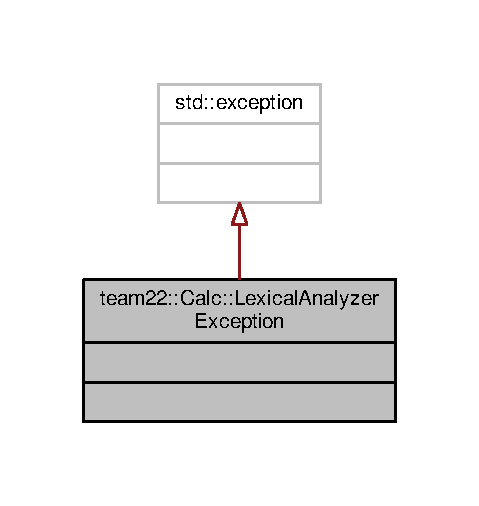
\includegraphics[width=230pt]{classteam22_1_1_calc_1_1_lexical_analyzer_exception__inherit__graph}
\end{center}
\end{figure}


Collaboration diagram for team22\+:\+:Calc\+:\+:Lexical\+Analyzer\+Exception\+:
\nopagebreak
\begin{figure}[H]
\begin{center}
\leavevmode
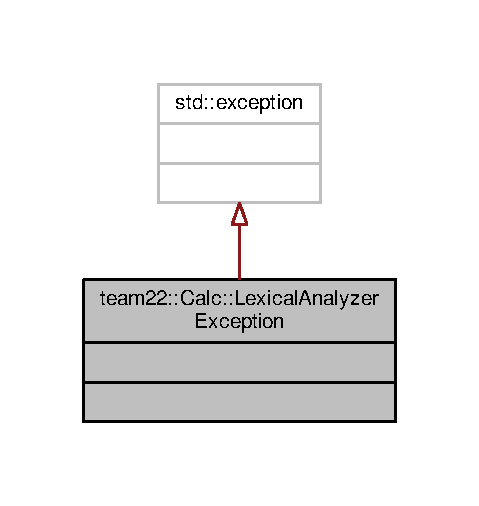
\includegraphics[width=230pt]{classteam22_1_1_calc_1_1_lexical_analyzer_exception__coll__graph}
\end{center}
\end{figure}


\subsection{Detailed Description}


Definition at line 15 of file Lexical\+Analyzer\+Exception.\+h.



The documentation for this class was generated from the following file\+:\begin{DoxyCompactItemize}
\item 
\hyperlink{_lexical_analyzer_exception_8h}{Lexical\+Analyzer\+Exception.\+h}\end{DoxyCompactItemize}

\hypertarget{classteam22_1_1_calc_1_1_lex_identification_observer}{}\section{team22\+:\+:Calc\+:\+:Lex\+Identification\+Observer Class Reference}
\label{classteam22_1_1_calc_1_1_lex_identification_observer}\index{team22\+::\+Calc\+::\+Lex\+Identification\+Observer@{team22\+::\+Calc\+::\+Lex\+Identification\+Observer}}


{\ttfamily \#include $<$Lex\+Identification\+Observer.\+h$>$}



Inheritance diagram for team22\+:\+:Calc\+:\+:Lex\+Identification\+Observer\+:
\nopagebreak
\begin{figure}[H]
\begin{center}
\leavevmode
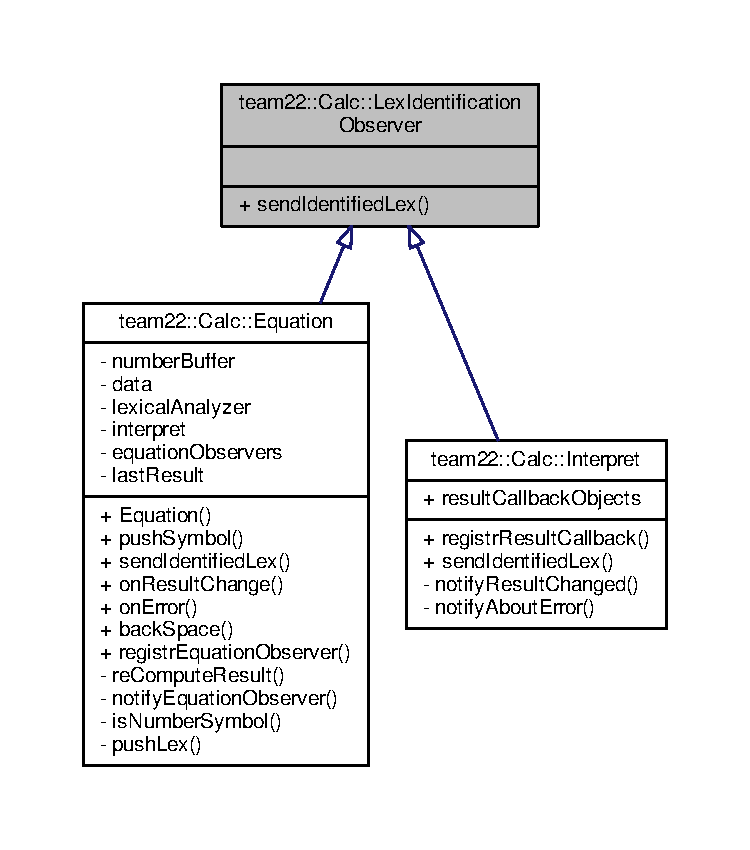
\includegraphics[width=350pt]{classteam22_1_1_calc_1_1_lex_identification_observer__inherit__graph}
\end{center}
\end{figure}


Collaboration diagram for team22\+:\+:Calc\+:\+:Lex\+Identification\+Observer\+:
\nopagebreak
\begin{figure}[H]
\begin{center}
\leavevmode
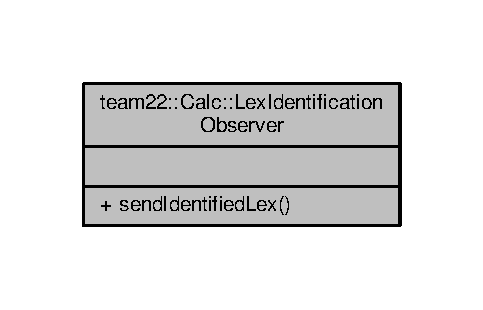
\includegraphics[width=232pt]{classteam22_1_1_calc_1_1_lex_identification_observer__coll__graph}
\end{center}
\end{figure}
\subsection*{Public Member Functions}
\begin{DoxyCompactItemize}
\item 
virtual void \hyperlink{classteam22_1_1_calc_1_1_lex_identification_observer_ac139f75c560625ec6fdb2e34cf0d4884}{send\+Identified\+Lex} (\hyperlink{classteam22_1_1_calc_1_1_lex}{Lex} lex)=0
\end{DoxyCompactItemize}


\subsection{Detailed Description}


Definition at line 15 of file Lex\+Identification\+Observer.\+h.



\subsection{Member Function Documentation}
\mbox{\Hypertarget{classteam22_1_1_calc_1_1_lex_identification_observer_ac139f75c560625ec6fdb2e34cf0d4884}\label{classteam22_1_1_calc_1_1_lex_identification_observer_ac139f75c560625ec6fdb2e34cf0d4884}} 
\index{team22\+::\+Calc\+::\+Lex\+Identification\+Observer@{team22\+::\+Calc\+::\+Lex\+Identification\+Observer}!send\+Identified\+Lex@{send\+Identified\+Lex}}
\index{send\+Identified\+Lex@{send\+Identified\+Lex}!team22\+::\+Calc\+::\+Lex\+Identification\+Observer@{team22\+::\+Calc\+::\+Lex\+Identification\+Observer}}
\subsubsection{\texorpdfstring{send\+Identified\+Lex()}{sendIdentifiedLex()}}
{\footnotesize\ttfamily virtual void team22\+::\+Calc\+::\+Lex\+Identification\+Observer\+::send\+Identified\+Lex (\begin{DoxyParamCaption}\item[{\hyperlink{classteam22_1_1_calc_1_1_lex}{Lex}}]{lex }\end{DoxyParamCaption})\hspace{0.3cm}{\ttfamily [pure virtual]}}



Implemented in \hyperlink{struct_lexical_analyzer_errors_test_ac943a4238a0eb77957e2027740603c44}{Lexical\+Analyzer\+Errors\+Test}, \hyperlink{classteam22_1_1_calc_1_1_equation_ad5768951865500ec7fc514f676de2851}{team22\+::\+Calc\+::\+Equation}, \hyperlink{classteam22_1_1_calc_1_1_interpret_a479c65c010f4ef1060049b684e5f7eb6}{team22\+::\+Calc\+::\+Interpret}, and \hyperlink{struct_lexical_analyzer_test_a1c412feae956dcdc6ca0519e361e8f64}{Lexical\+Analyzer\+Test}.



The documentation for this class was generated from the following file\+:\begin{DoxyCompactItemize}
\item 
src/\hyperlink{_lex_identification_observer_8h}{Lex\+Identification\+Observer.\+h}\end{DoxyCompactItemize}

\hypertarget{classteam22_1_1_calc_1_1_result_observer}{}\section{team22\+:\+:Calc\+:\+:Result\+Observer Class Reference}
\label{classteam22_1_1_calc_1_1_result_observer}\index{team22\+::\+Calc\+::\+Result\+Observer@{team22\+::\+Calc\+::\+Result\+Observer}}


{\ttfamily \#include $<$Result\+Observer.\+h$>$}



Inheritance diagram for team22\+:\+:Calc\+:\+:Result\+Observer\+:
\nopagebreak
\begin{figure}[H]
\begin{center}
\leavevmode
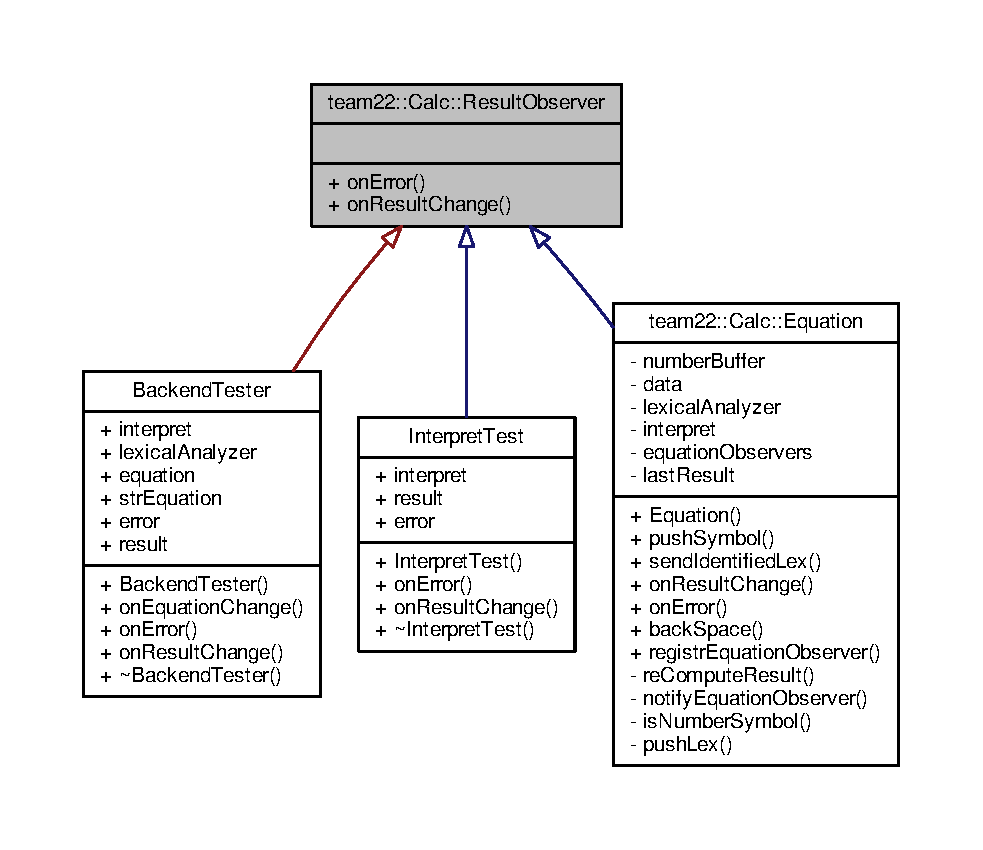
\includegraphics[width=229pt]{classteam22_1_1_calc_1_1_result_observer__inherit__graph}
\end{center}
\end{figure}


Collaboration diagram for team22\+:\+:Calc\+:\+:Result\+Observer\+:
\nopagebreak
\begin{figure}[H]
\begin{center}
\leavevmode
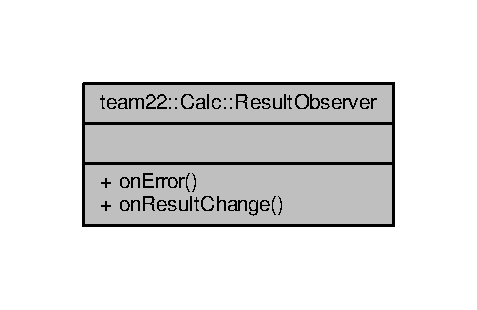
\includegraphics[width=229pt]{classteam22_1_1_calc_1_1_result_observer__coll__graph}
\end{center}
\end{figure}
\subsection*{Public Member Functions}
\begin{DoxyCompactItemize}
\item 
virtual void \hyperlink{classteam22_1_1_calc_1_1_result_observer_ad36cf8df89853d60f91094800c01d329}{on\+Error} (\hyperlink{class_interpret_exception}{Interpret\+Exception} exception)=0
\item 
virtual void \hyperlink{classteam22_1_1_calc_1_1_result_observer_aa04007df3aa8a499c3a511f549238285}{on\+Result\+Change} (Math\+::\+Number result)=0
\end{DoxyCompactItemize}


\subsection{Detailed Description}


Definition at line 15 of file Result\+Observer.\+h.



\subsection{Member Function Documentation}
\mbox{\Hypertarget{classteam22_1_1_calc_1_1_result_observer_ad36cf8df89853d60f91094800c01d329}\label{classteam22_1_1_calc_1_1_result_observer_ad36cf8df89853d60f91094800c01d329}} 
\index{team22\+::\+Calc\+::\+Result\+Observer@{team22\+::\+Calc\+::\+Result\+Observer}!on\+Error@{on\+Error}}
\index{on\+Error@{on\+Error}!team22\+::\+Calc\+::\+Result\+Observer@{team22\+::\+Calc\+::\+Result\+Observer}}
\subsubsection{\texorpdfstring{on\+Error()}{onError()}}
{\footnotesize\ttfamily virtual void team22\+::\+Calc\+::\+Result\+Observer\+::on\+Error (\begin{DoxyParamCaption}\item[{\hyperlink{class_interpret_exception}{Interpret\+Exception}}]{exception }\end{DoxyParamCaption})\hspace{0.3cm}{\ttfamily [pure virtual]}}

Callback volaný pokud vznikla chyba při výpočtu 
\begin{DoxyParams}{Parameters}
{\em \hyperlink{class_interpret_exception}{Interpret\+Exception}} & \\
\hline
\end{DoxyParams}


Implemented in \hyperlink{classteam22_1_1_calc_1_1_equation_a4e7a0614867931bcc714440441cdd894}{team22\+::\+Calc\+::\+Equation}.

\mbox{\Hypertarget{classteam22_1_1_calc_1_1_result_observer_aa04007df3aa8a499c3a511f549238285}\label{classteam22_1_1_calc_1_1_result_observer_aa04007df3aa8a499c3a511f549238285}} 
\index{team22\+::\+Calc\+::\+Result\+Observer@{team22\+::\+Calc\+::\+Result\+Observer}!on\+Result\+Change@{on\+Result\+Change}}
\index{on\+Result\+Change@{on\+Result\+Change}!team22\+::\+Calc\+::\+Result\+Observer@{team22\+::\+Calc\+::\+Result\+Observer}}
\subsubsection{\texorpdfstring{on\+Result\+Change()}{onResultChange()}}
{\footnotesize\ttfamily virtual void team22\+::\+Calc\+::\+Result\+Observer\+::on\+Result\+Change (\begin{DoxyParamCaption}\item[{Math\+::\+Number}]{result }\end{DoxyParamCaption})\hspace{0.3cm}{\ttfamily [pure virtual]}}

Callback volaný při změně výsledku 
\begin{DoxyParams}{Parameters}
{\em result} & \\
\hline
\end{DoxyParams}


Implemented in \hyperlink{classteam22_1_1_calc_1_1_equation_a302c295e099f589897a1bad4b02d3de8}{team22\+::\+Calc\+::\+Equation}.



The documentation for this class was generated from the following file\+:\begin{DoxyCompactItemize}
\item 
\hyperlink{_result_observer_8h}{Result\+Observer.\+h}\end{DoxyCompactItemize}

\hypertarget{unionteam22_1_1_calc_1_1_lex_1_1_value}{}\section{team22\+:\+:Calc\+:\+:Lex\+:\+:Value Union Reference}
\label{unionteam22_1_1_calc_1_1_lex_1_1_value}\index{team22\+::\+Calc\+::\+Lex\+::\+Value@{team22\+::\+Calc\+::\+Lex\+::\+Value}}


reprezentace hodnoty lexému  




{\ttfamily \#include $<$Lex.\+h$>$}



Collaboration diagram for team22\+:\+:Calc\+:\+:Lex\+:\+:Value\+:
\nopagebreak
\begin{figure}[H]
\begin{center}
\leavevmode
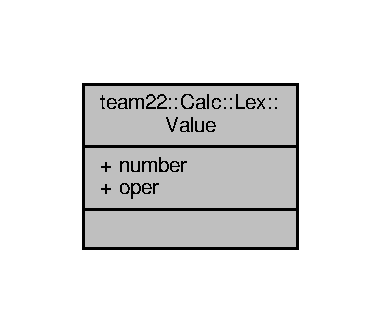
\includegraphics[width=197pt]{unionteam22_1_1_calc_1_1_lex_1_1_value__coll__graph}
\end{center}
\end{figure}
\subsection*{Public Attributes}
\begin{DoxyCompactItemize}
\item 
\hyperlink{classteam22_1_1_math_1_1_number}{Math\+::\+Number} \hyperlink{unionteam22_1_1_calc_1_1_lex_1_1_value_a86e2e3ea0c887ca50885bcdb8f1ec5ce}{number} \{0\}
\item 
\hyperlink{classteam22_1_1_calc_1_1_lex_a61d29fc4878a3b36d2de2f13c56ed932}{Operator} \hyperlink{unionteam22_1_1_calc_1_1_lex_1_1_value_ade46fa860d495ce4d431d3934210579d}{oper}
\end{DoxyCompactItemize}


\subsection{Detailed Description}
reprezentace hodnoty lexému 

Definition at line 67 of file Lex.\+h.



\subsection{Member Data Documentation}
\mbox{\Hypertarget{unionteam22_1_1_calc_1_1_lex_1_1_value_a86e2e3ea0c887ca50885bcdb8f1ec5ce}\label{unionteam22_1_1_calc_1_1_lex_1_1_value_a86e2e3ea0c887ca50885bcdb8f1ec5ce}} 
\index{team22\+::\+Calc\+::\+Lex\+::\+Value@{team22\+::\+Calc\+::\+Lex\+::\+Value}!number@{number}}
\index{number@{number}!team22\+::\+Calc\+::\+Lex\+::\+Value@{team22\+::\+Calc\+::\+Lex\+::\+Value}}
\subsubsection{\texorpdfstring{number}{number}}
{\footnotesize\ttfamily \hyperlink{classteam22_1_1_math_1_1_number}{Math\+::\+Number} team22\+::\+Calc\+::\+Lex\+::\+Value\+::number \{0\}}



Definition at line 69 of file Lex.\+h.



Referenced by team22\+::\+Calc\+::\+Lex\+::get\+As\+Number(), and team22\+::\+Calc\+::\+Lex\+::\+Lex().

\mbox{\Hypertarget{unionteam22_1_1_calc_1_1_lex_1_1_value_ade46fa860d495ce4d431d3934210579d}\label{unionteam22_1_1_calc_1_1_lex_1_1_value_ade46fa860d495ce4d431d3934210579d}} 
\index{team22\+::\+Calc\+::\+Lex\+::\+Value@{team22\+::\+Calc\+::\+Lex\+::\+Value}!oper@{oper}}
\index{oper@{oper}!team22\+::\+Calc\+::\+Lex\+::\+Value@{team22\+::\+Calc\+::\+Lex\+::\+Value}}
\subsubsection{\texorpdfstring{oper}{oper}}
{\footnotesize\ttfamily \hyperlink{classteam22_1_1_calc_1_1_lex_a61d29fc4878a3b36d2de2f13c56ed932}{Operator} team22\+::\+Calc\+::\+Lex\+::\+Value\+::oper}



Definition at line 70 of file Lex.\+h.



Referenced by team22\+::\+Calc\+::\+Lex\+::get\+As\+Operator(), and team22\+::\+Calc\+::\+Lex\+::\+Lex().



The documentation for this union was generated from the following file\+:\begin{DoxyCompactItemize}
\item 
\hyperlink{_lex_8h}{Lex.\+h}\end{DoxyCompactItemize}

\chapter{File Documentation}
\hypertarget{_equation_8cpp}{}\section{src/\+Equation.cpp File Reference}
\label{_equation_8cpp}\index{src/\+Equation.\+cpp@{src/\+Equation.\+cpp}}
{\ttfamily \#include \char`\"{}Equation.\+h\char`\"{}}\newline
Include dependency graph for Equation.\+cpp\+:
\nopagebreak
\begin{figure}[H]
\begin{center}
\leavevmode
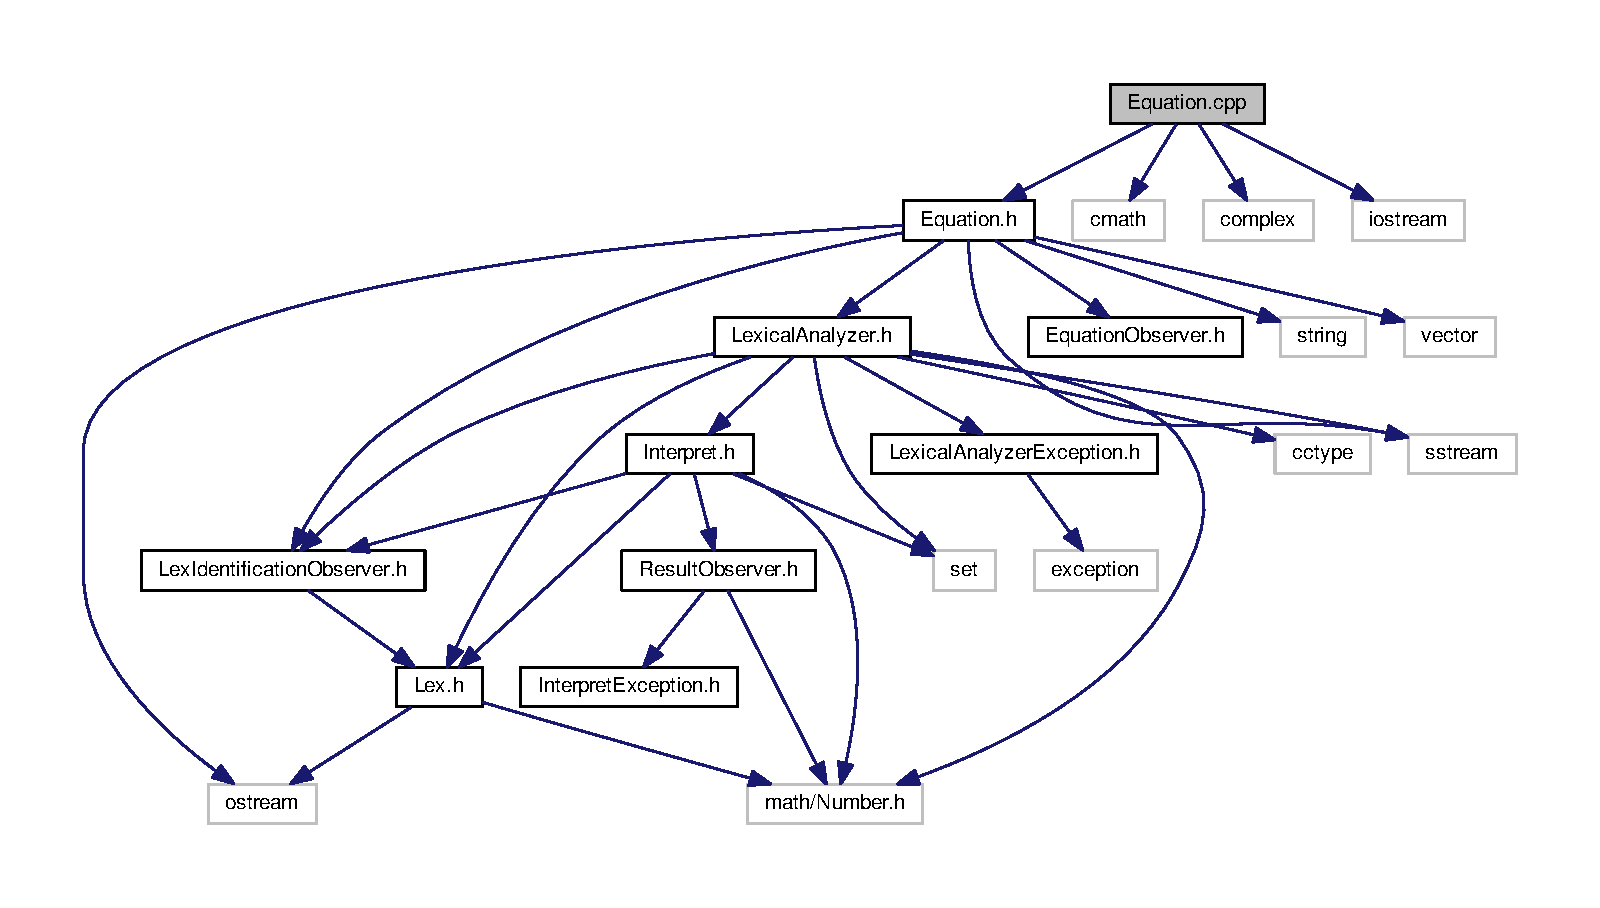
\includegraphics[width=350pt]{_equation_8cpp__incl}
\end{center}
\end{figure}


\subsection{Detailed Description}
U\+T\+F-\/8 \begin{DoxyDate}{Date}
8.\+4.\+18 
\end{DoxyDate}
\begin{DoxyAuthor}{Author}
Adam Mátl \href{mailto:xmatla00@stud.fit.vutbr.cz}{\tt xmatla00@stud.\+fit.\+vutbr.\+cz} \href{mailto:matla@matla.cz}{\tt matla@matla.\+cz} 
\end{DoxyAuthor}

\hypertarget{_equation_8h}{}\section{src/\+Equation.h File Reference}
\label{_equation_8h}\index{src/\+Equation.\+h@{src/\+Equation.\+h}}
{\ttfamily \#include \char`\"{}Lex\+Identification\+Observer.\+h\char`\"{}}\newline
{\ttfamily \#include \char`\"{}Lexical\+Analyzer.\+h\char`\"{}}\newline
{\ttfamily \#include \char`\"{}Equation\+Observer.\+h\char`\"{}}\newline
{\ttfamily \#include $<$string$>$}\newline
{\ttfamily \#include $<$vector$>$}\newline
{\ttfamily \#include $<$sstream$>$}\newline
{\ttfamily \#include $<$ostream$>$}\newline
Include dependency graph for Equation.\+h\+:
\nopagebreak
\begin{figure}[H]
\begin{center}
\leavevmode
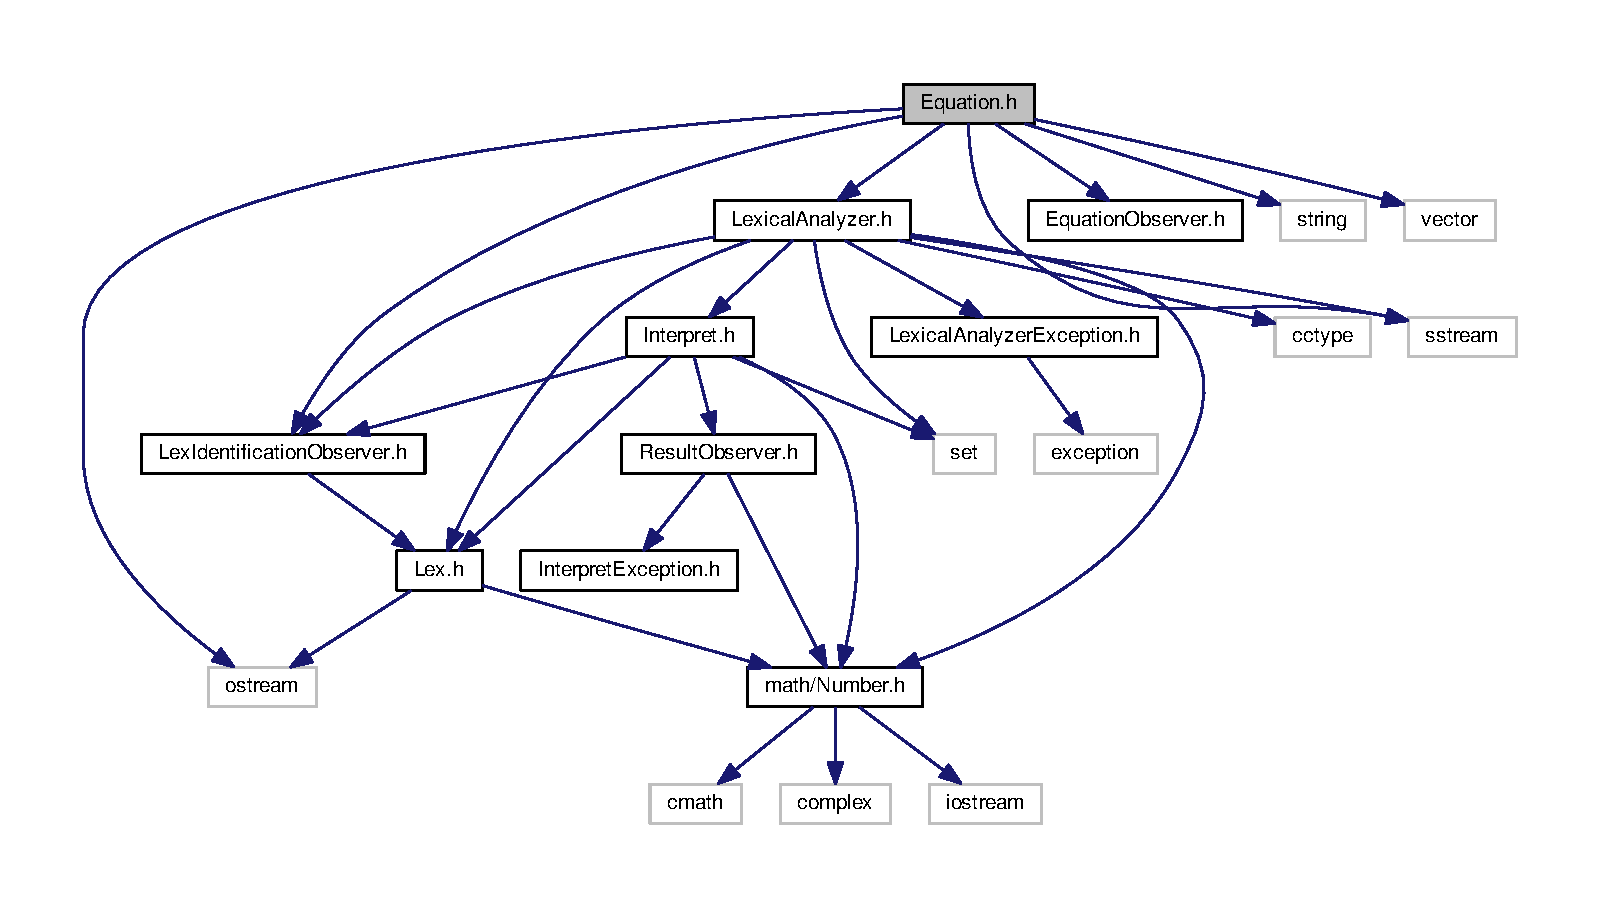
\includegraphics[width=350pt]{_equation_8h__incl}
\end{center}
\end{figure}
This graph shows which files directly or indirectly include this file\+:
\nopagebreak
\begin{figure}[H]
\begin{center}
\leavevmode
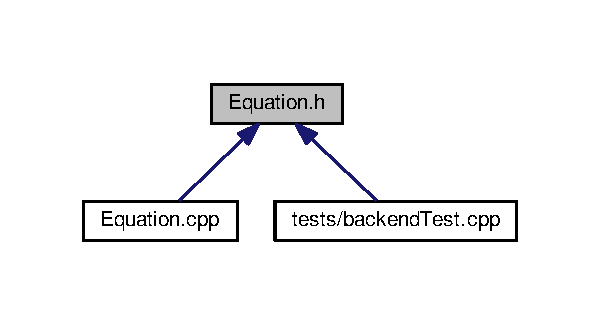
\includegraphics[width=322pt]{_equation_8h__dep__incl}
\end{center}
\end{figure}
\subsection*{Classes}
\begin{DoxyCompactItemize}
\item 
class \hyperlink{classteam22_1_1_calc_1_1_equation}{team22\+::\+Calc\+::\+Equation}
\begin{DoxyCompactList}\small\item\em Třída reprezentující rovnici. \end{DoxyCompactList}\end{DoxyCompactItemize}
\subsection*{Namespaces}
\begin{DoxyCompactItemize}
\item 
 \hyperlink{namespaceteam22_1_1_calc}{team22\+::\+Calc}
\end{DoxyCompactItemize}


\subsection{Detailed Description}
U\+T\+F-\/8 \begin{DoxyDate}{Date}
8.\+4.\+18 
\end{DoxyDate}
\begin{DoxyAuthor}{Author}
Adam Mátl \href{mailto:xmatla00@stud.fit.vutbr.cz}{\tt xmatla00@stud.\+fit.\+vutbr.\+cz} \href{mailto:matla@matla.cz}{\tt matla@matla.\+cz} 
\end{DoxyAuthor}

\hypertarget{_equation_observer_8h}{}\section{Equation\+Observer.\+h File Reference}
\label{_equation_observer_8h}\index{Equation\+Observer.\+h@{Equation\+Observer.\+h}}
This graph shows which files directly or indirectly include this file\+:
\nopagebreak
\begin{figure}[H]
\begin{center}
\leavevmode
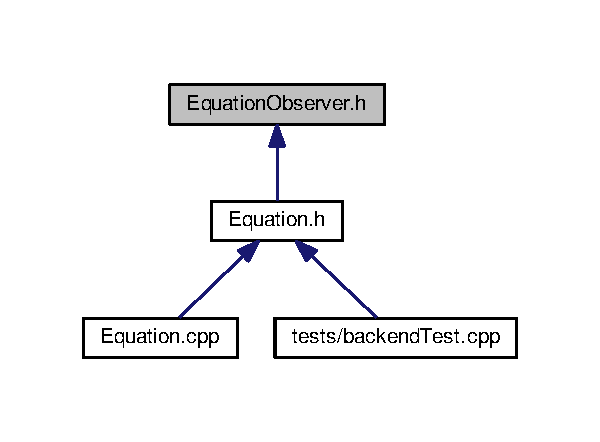
\includegraphics[width=183pt]{_equation_observer_8h__dep__incl}
\end{center}
\end{figure}
\subsection*{Classes}
\begin{DoxyCompactItemize}
\item 
class \hyperlink{classteam22_1_1_calc_1_1_equation_observer}{team22\+::\+Calc\+::\+Equation\+Observer}
\end{DoxyCompactItemize}
\subsection*{Namespaces}
\begin{DoxyCompactItemize}
\item 
 \hyperlink{namespaceteam22_1_1_calc}{team22\+::\+Calc}
\end{DoxyCompactItemize}


\subsection{Detailed Description}
U\+T\+F-\/8 \begin{DoxyDate}{Date}
8.\+4.\+18 
\end{DoxyDate}
\begin{DoxyAuthor}{Author}
Adam Mátl \href{mailto:xmatla00@stud.fit.vutbr.cz}{\tt xmatla00@stud.\+fit.\+vutbr.\+cz} \href{mailto:matla@matla.cz}{\tt matla@matla.\+cz} 
\end{DoxyAuthor}

\hypertarget{_interpret_8cpp}{}\section{src/\+Interpret.cpp File Reference}
\label{_interpret_8cpp}\index{src/\+Interpret.\+cpp@{src/\+Interpret.\+cpp}}
{\ttfamily \#include \char`\"{}Interpret.\+h\char`\"{}}\newline
Include dependency graph for Interpret.\+cpp\+:
\nopagebreak
\begin{figure}[H]
\begin{center}
\leavevmode
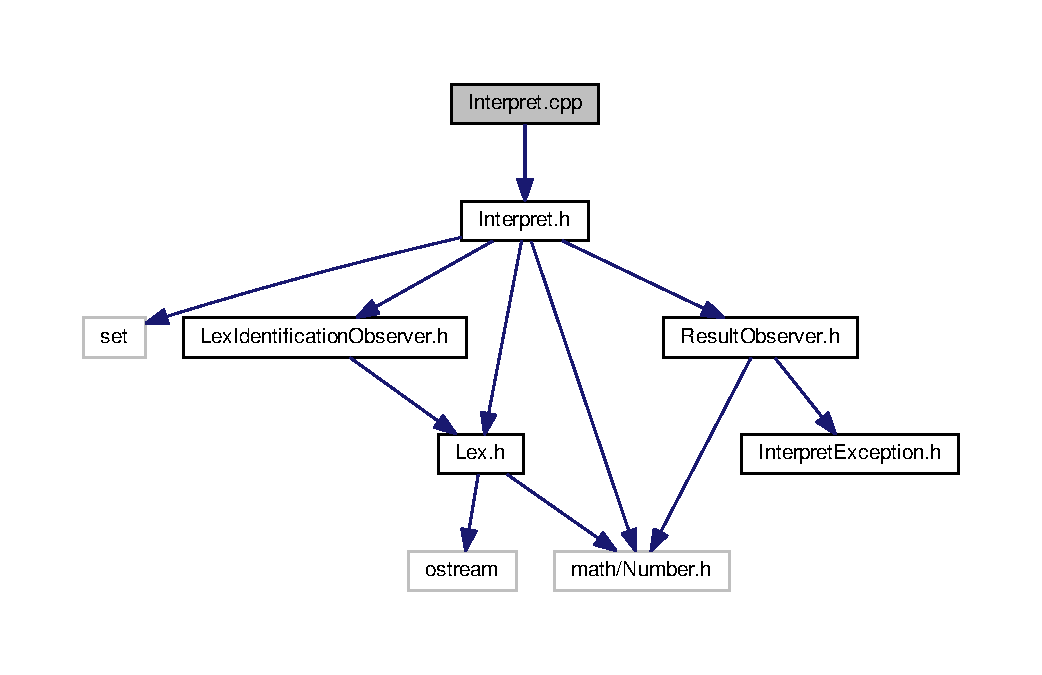
\includegraphics[width=350pt]{_interpret_8cpp__incl}
\end{center}
\end{figure}


\subsection{Detailed Description}
U\+T\+F-\/8 \begin{DoxyDate}{Date}
22.\+3.\+18 
\end{DoxyDate}
\begin{DoxyAuthor}{Author}
Adam Mátl \href{mailto:xmatla00@stud.fit.vutbr.cz}{\tt xmatla00@stud.\+fit.\+vutbr.\+cz} \href{mailto:matla@matla.cz}{\tt matla@matla.\+cz} 
\end{DoxyAuthor}

\hypertarget{_interpret_8h}{}\section{src/\+Interpret.h File Reference}
\label{_interpret_8h}\index{src/\+Interpret.\+h@{src/\+Interpret.\+h}}
{\ttfamily \#include $<$set$>$}\newline
{\ttfamily \#include \char`\"{}Lex\+Identification\+Observer.\+h\char`\"{}}\newline
{\ttfamily \#include \char`\"{}Lex.\+h\char`\"{}}\newline
{\ttfamily \#include \char`\"{}Result\+Observer.\+h\char`\"{}}\newline
{\ttfamily \#include \char`\"{}math/\+Number.\+h\char`\"{}}\newline
Include dependency graph for Interpret.\+h\+:
\nopagebreak
\begin{figure}[H]
\begin{center}
\leavevmode
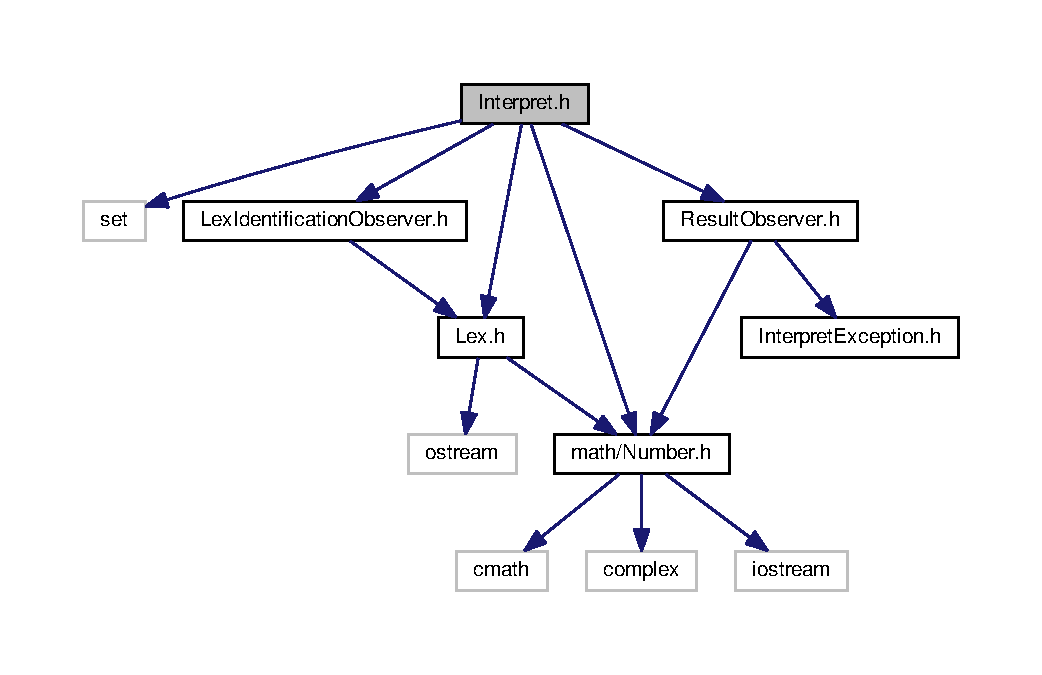
\includegraphics[width=350pt]{_interpret_8h__incl}
\end{center}
\end{figure}
This graph shows which files directly or indirectly include this file\+:
\nopagebreak
\begin{figure}[H]
\begin{center}
\leavevmode
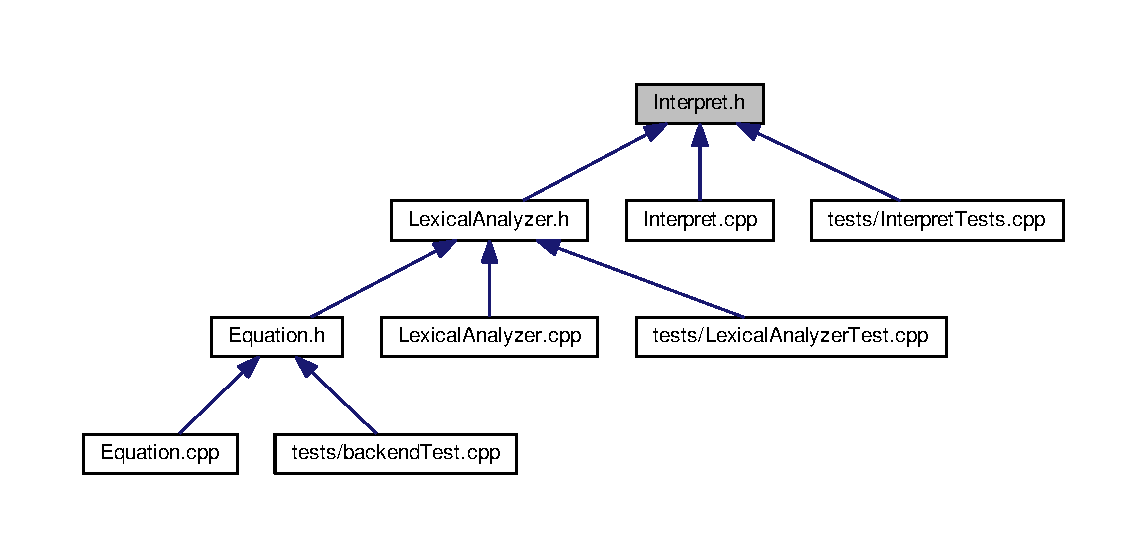
\includegraphics[width=350pt]{_interpret_8h__dep__incl}
\end{center}
\end{figure}
\subsection*{Classes}
\begin{DoxyCompactItemize}
\item 
class \hyperlink{classteam22_1_1_calc_1_1_interpret}{team22\+::\+Calc\+::\+Interpret}
\end{DoxyCompactItemize}
\subsection*{Namespaces}
\begin{DoxyCompactItemize}
\item 
 \hyperlink{namespaceteam22_1_1_calc}{team22\+::\+Calc}
\end{DoxyCompactItemize}


\subsection{Detailed Description}
U\+T\+F-\/8 \begin{DoxyDate}{Date}
22.\+3.\+18 
\end{DoxyDate}
\begin{DoxyAuthor}{Author}
Adam Mátl \href{mailto:xmatla00@stud.fit.vutbr.cz}{\tt xmatla00@stud.\+fit.\+vutbr.\+cz} \href{mailto:matla@matla.cz}{\tt matla@matla.\+cz} 
\end{DoxyAuthor}

\hypertarget{_interpret_exception_8h}{}\section{src/\+Interpret\+Exception.h File Reference}
\label{_interpret_exception_8h}\index{src/\+Interpret\+Exception.\+h@{src/\+Interpret\+Exception.\+h}}
This graph shows which files directly or indirectly include this file\+:
\nopagebreak
\begin{figure}[H]
\begin{center}
\leavevmode
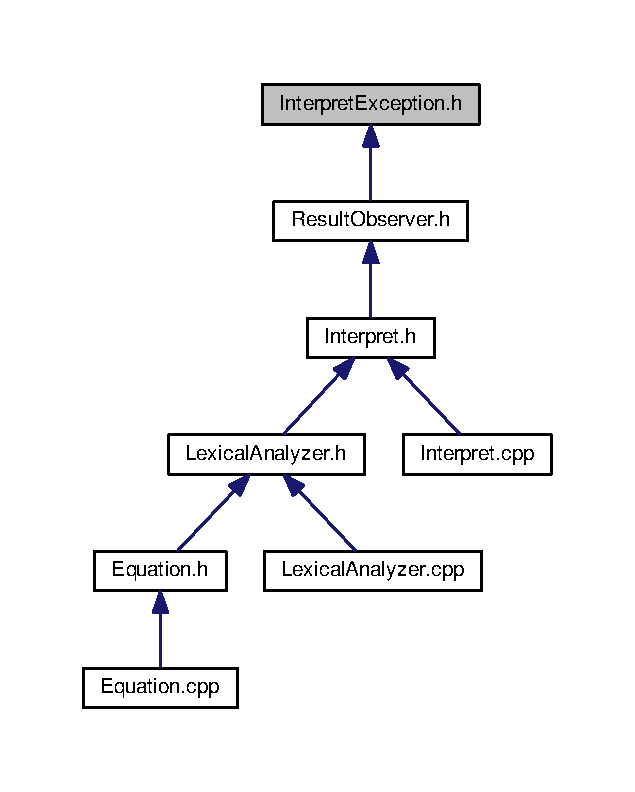
\includegraphics[width=350pt]{_interpret_exception_8h__dep__incl}
\end{center}
\end{figure}
\subsection*{Classes}
\begin{DoxyCompactItemize}
\item 
class \hyperlink{class_interpret_exception}{Interpret\+Exception}
\end{DoxyCompactItemize}


\subsection{Detailed Description}
U\+T\+F-\/8 \begin{DoxyDate}{Date}
29.\+3.\+18 
\end{DoxyDate}
\begin{DoxyAuthor}{Author}
Adam Mátl \href{mailto:xmatla00@stud.fit.vutbr.cz}{\tt xmatla00@stud.\+fit.\+vutbr.\+cz} \href{mailto:matla@matla.cz}{\tt matla@matla.\+cz} 
\end{DoxyAuthor}

\hypertarget{_lex_8cpp}{}\section{Lex.\+cpp File Reference}
\label{_lex_8cpp}\index{Lex.\+cpp@{Lex.\+cpp}}
{\ttfamily \#include \char`\"{}Lex.\+h\char`\"{}}\newline
{\ttfamily \#include \char`\"{}Lex\+Exception.\+h\char`\"{}}\newline
Include dependency graph for Lex.\+cpp\+:
\nopagebreak
\begin{figure}[H]
\begin{center}
\leavevmode
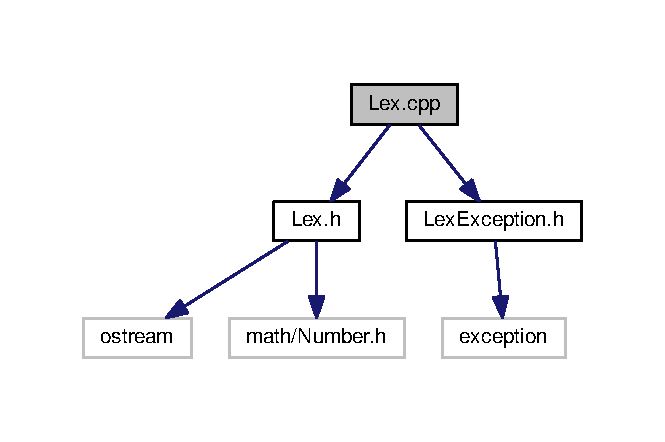
\includegraphics[width=319pt]{_lex_8cpp__incl}
\end{center}
\end{figure}


\subsection{Detailed Description}
U\+T\+F-\/8 \begin{DoxyDate}{Date}
22.\+3.\+18 
\end{DoxyDate}
\begin{DoxyAuthor}{Author}
Adam Mátl \href{mailto:xmatla00@stud.fit.vutbr.cz}{\tt xmatla00@stud.\+fit.\+vutbr.\+cz} \href{mailto:matla@matla.cz}{\tt matla@matla.\+cz} 
\end{DoxyAuthor}

\hypertarget{_lex_8h}{}\section{Lex.\+h File Reference}
\label{_lex_8h}\index{Lex.\+h@{Lex.\+h}}
{\ttfamily \#include $<$ostream$>$}\newline
{\ttfamily \#include \char`\"{}math/\+Number.\+h\char`\"{}}\newline
Include dependency graph for Lex.\+h\+:
\nopagebreak
\begin{figure}[H]
\begin{center}
\leavevmode
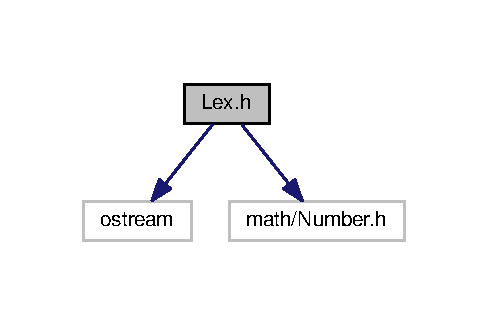
\includegraphics[width=234pt]{_lex_8h__incl}
\end{center}
\end{figure}
This graph shows which files directly or indirectly include this file\+:
\nopagebreak
\begin{figure}[H]
\begin{center}
\leavevmode
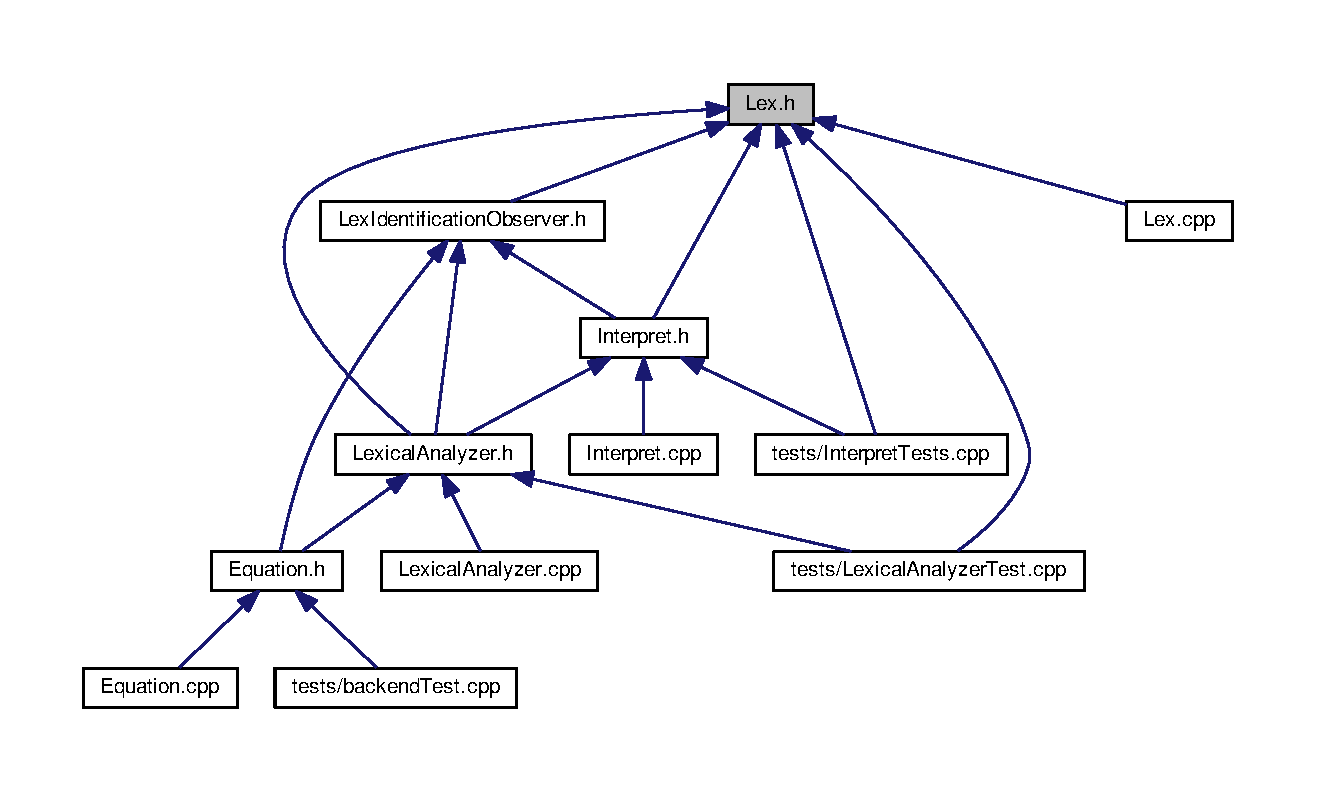
\includegraphics[width=350pt]{_lex_8h__dep__incl}
\end{center}
\end{figure}
\subsection*{Classes}
\begin{DoxyCompactItemize}
\item 
class \hyperlink{classteam22_1_1_calc_1_1_lex}{team22\+::\+Calc\+::\+Lex}
\begin{DoxyCompactList}\small\item\em Reprezentace lexému kalkulačky tedy čísla nebo operace. \end{DoxyCompactList}\item 
union \hyperlink{unionteam22_1_1_calc_1_1_lex_1_1_value}{team22\+::\+Calc\+::\+Lex\+::\+Value}
\begin{DoxyCompactList}\small\item\em reprezentace hodnoty lexému \end{DoxyCompactList}\end{DoxyCompactItemize}
\subsection*{Namespaces}
\begin{DoxyCompactItemize}
\item 
 \hyperlink{namespaceteam22_1_1_calc}{team22\+::\+Calc}
\end{DoxyCompactItemize}


\subsection{Detailed Description}
U\+T\+F-\/8 \begin{DoxyDate}{Date}
22.\+3.\+18 
\end{DoxyDate}
\begin{DoxyAuthor}{Author}
Adam Mátl \href{mailto:xmatla00@stud.fit.vutbr.cz}{\tt xmatla00@stud.\+fit.\+vutbr.\+cz} \href{mailto:matla@matla.cz}{\tt matla@matla.\+cz} 
\end{DoxyAuthor}

\hypertarget{_lex_exception_8h}{}\section{src/\+Lex\+Exception.h File Reference}
\label{_lex_exception_8h}\index{src/\+Lex\+Exception.\+h@{src/\+Lex\+Exception.\+h}}
{\ttfamily \#include $<$exception$>$}\newline
Include dependency graph for Lex\+Exception.\+h\+:
\nopagebreak
\begin{figure}[H]
\begin{center}
\leavevmode
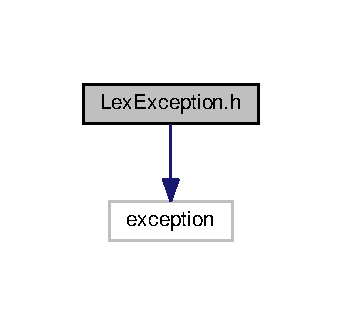
\includegraphics[width=181pt]{_lex_exception_8h__incl}
\end{center}
\end{figure}
This graph shows which files directly or indirectly include this file\+:
\nopagebreak
\begin{figure}[H]
\begin{center}
\leavevmode
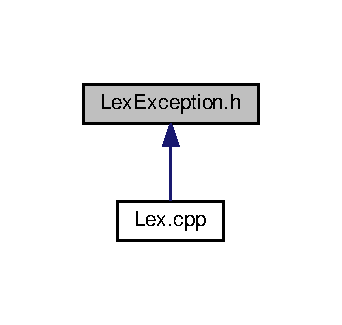
\includegraphics[width=181pt]{_lex_exception_8h__dep__incl}
\end{center}
\end{figure}
\subsection*{Classes}
\begin{DoxyCompactItemize}
\item 
class \hyperlink{classteam22_1_1_calc_1_1_lex_exception}{team22\+::\+Calc\+::\+Lex\+Exception}
\end{DoxyCompactItemize}
\subsection*{Namespaces}
\begin{DoxyCompactItemize}
\item 
 \hyperlink{namespaceteam22_1_1_calc}{team22\+::\+Calc}
\end{DoxyCompactItemize}


\subsection{Detailed Description}
U\+T\+F-\/8 \begin{DoxyDate}{Date}
22.\+3.\+18 
\end{DoxyDate}
\begin{DoxyAuthor}{Author}
Adam Mátl \href{mailto:xmatla00@stud.fit.vutbr.cz}{\tt xmatla00@stud.\+fit.\+vutbr.\+cz} \href{mailto:matla@matla.cz}{\tt matla@matla.\+cz} 
\end{DoxyAuthor}

\hypertarget{_lexical_analyzer_8cpp}{}\section{Lexical\+Analyzer.\+cpp File Reference}
\label{_lexical_analyzer_8cpp}\index{Lexical\+Analyzer.\+cpp@{Lexical\+Analyzer.\+cpp}}
{\ttfamily \#include \char`\"{}Lexical\+Analyzer.\+h\char`\"{}}\newline
Include dependency graph for Lexical\+Analyzer.\+cpp\+:
\nopagebreak
\begin{figure}[H]
\begin{center}
\leavevmode
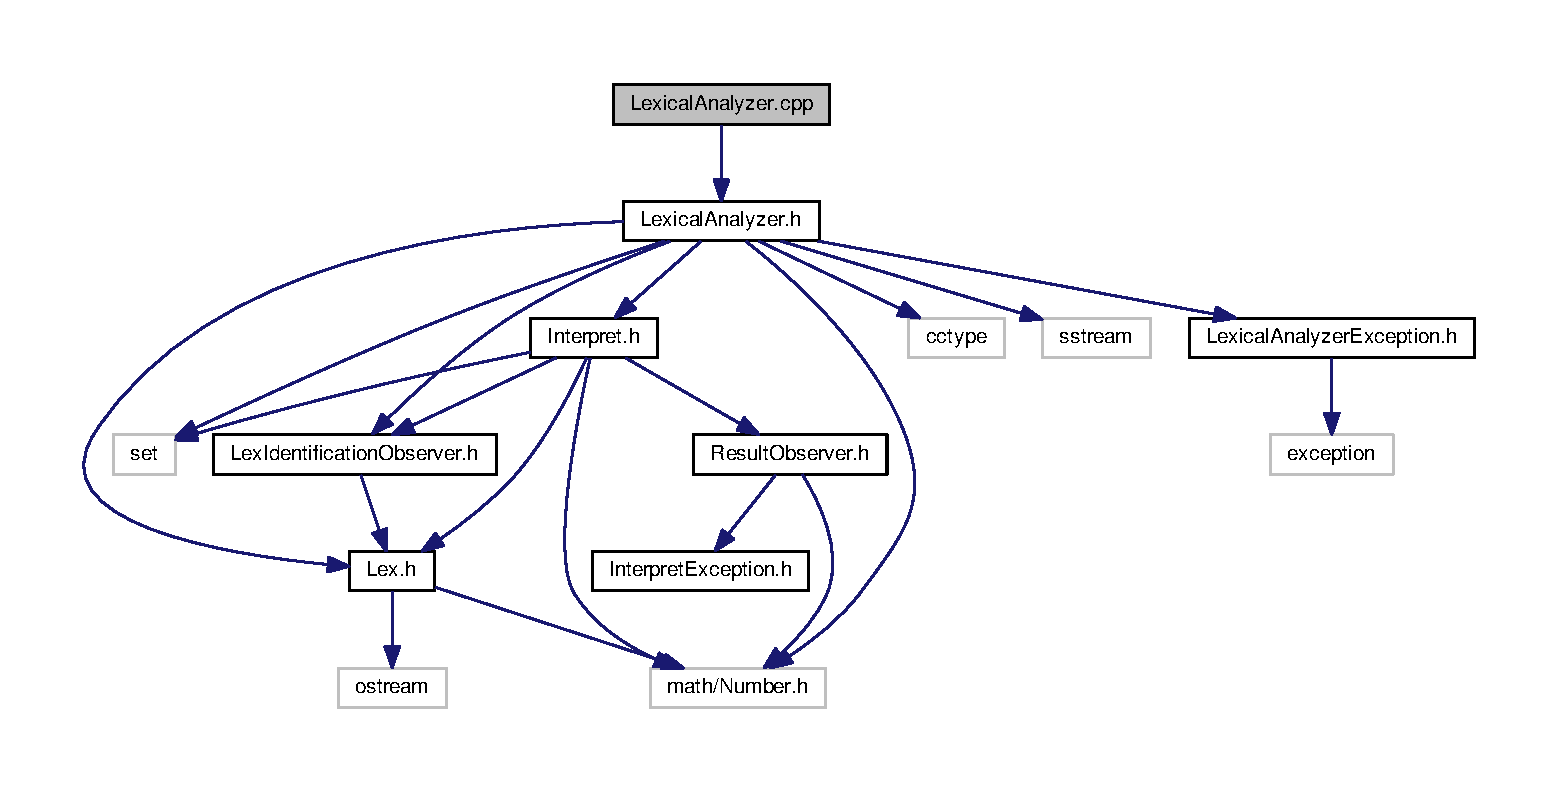
\includegraphics[width=350pt]{_lexical_analyzer_8cpp__incl}
\end{center}
\end{figure}
\subsection*{Namespaces}
\begin{DoxyCompactItemize}
\item 
 \hyperlink{namespaceteam22_1_1_calc}{team22\+::\+Calc}
\end{DoxyCompactItemize}


\subsection{Detailed Description}
U\+T\+F-\/8 \begin{DoxyDate}{Date}
28.\+3.\+18 
\end{DoxyDate}
\begin{DoxyAuthor}{Author}
Adam Mátl \href{mailto:xmatla00@stud.fit.vutbr.cz}{\tt xmatla00@stud.\+fit.\+vutbr.\+cz} \href{mailto:matla@matla.cz}{\tt matla@matla.\+cz}, Jiří Čechák \href{mailto:xcecha04@stud.fit.vutbr.cz}{\tt xcecha04@stud.\+fit.\+vutbr.\+cz} 
\end{DoxyAuthor}

\hypertarget{_lexical_analyzer_8h}{}\section{Lexical\+Analyzer.\+h File Reference}
\label{_lexical_analyzer_8h}\index{Lexical\+Analyzer.\+h@{Lexical\+Analyzer.\+h}}
{\ttfamily \#include $<$set$>$}\newline
{\ttfamily \#include $<$cctype$>$}\newline
{\ttfamily \#include $<$sstream$>$}\newline
{\ttfamily \#include \char`\"{}Lex.\+h\char`\"{}}\newline
{\ttfamily \#include \char`\"{}math/\+Number.\+h\char`\"{}}\newline
{\ttfamily \#include \char`\"{}Interpret.\+h\char`\"{}}\newline
{\ttfamily \#include \char`\"{}Lex\+Identification\+Observer.\+h\char`\"{}}\newline
{\ttfamily \#include \char`\"{}Lexical\+Analyzer\+Exception.\+h\char`\"{}}\newline
Include dependency graph for Lexical\+Analyzer.\+h\+:
\nopagebreak
\begin{figure}[H]
\begin{center}
\leavevmode
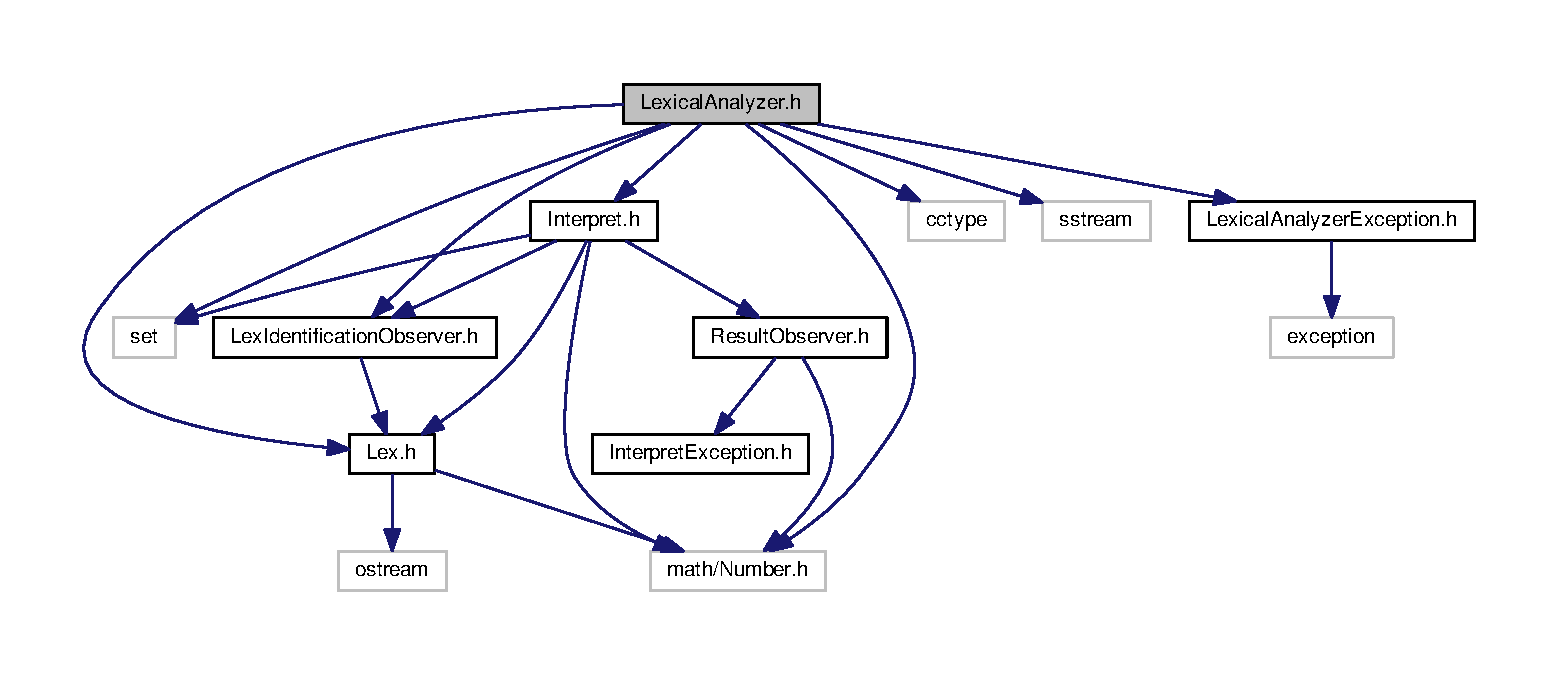
\includegraphics[width=350pt]{_lexical_analyzer_8h__incl}
\end{center}
\end{figure}
This graph shows which files directly or indirectly include this file\+:
\nopagebreak
\begin{figure}[H]
\begin{center}
\leavevmode
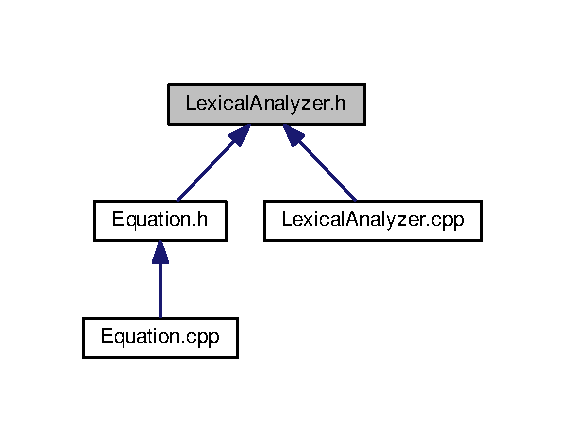
\includegraphics[width=271pt]{_lexical_analyzer_8h__dep__incl}
\end{center}
\end{figure}
\subsection*{Classes}
\begin{DoxyCompactItemize}
\item 
class \hyperlink{classteam22_1_1_calc_1_1_lexical_analyzer}{team22\+::\+Calc\+::\+Lexical\+Analyzer}
\end{DoxyCompactItemize}
\subsection*{Namespaces}
\begin{DoxyCompactItemize}
\item 
 \hyperlink{namespaceteam22_1_1_calc}{team22\+::\+Calc}
\end{DoxyCompactItemize}


\subsection{Detailed Description}
U\+T\+F-\/8 \begin{DoxyDate}{Date}
28.\+3.\+18 
\end{DoxyDate}
\begin{DoxyAuthor}{Author}
Adam Mátl \href{mailto:xmatla00@stud.fit.vutbr.cz}{\tt xmatla00@stud.\+fit.\+vutbr.\+cz} \href{mailto:matla@matla.cz}{\tt matla@matla.\+cz}, Jiří Čechák \href{mailto:xcecha04@stud.fit.vutbr.cz}{\tt xcecha04@stud.\+fit.\+vutbr.\+cz} 
\end{DoxyAuthor}

\hypertarget{_lexical_analyzer_exception_8h}{}\section{Lexical\+Analyzer\+Exception.\+h File Reference}
\label{_lexical_analyzer_exception_8h}\index{Lexical\+Analyzer\+Exception.\+h@{Lexical\+Analyzer\+Exception.\+h}}
{\ttfamily \#include $<$exception$>$}\newline
Include dependency graph for Lexical\+Analyzer\+Exception.\+h\+:
\nopagebreak
\begin{figure}[H]
\begin{center}
\leavevmode
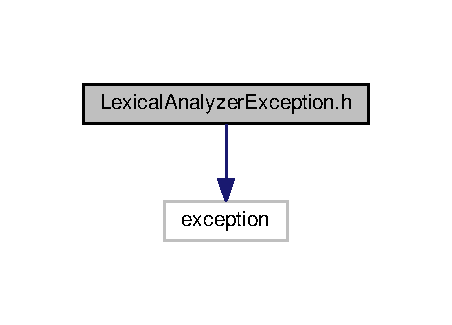
\includegraphics[width=217pt]{_lexical_analyzer_exception_8h__incl}
\end{center}
\end{figure}
This graph shows which files directly or indirectly include this file\+:
\nopagebreak
\begin{figure}[H]
\begin{center}
\leavevmode
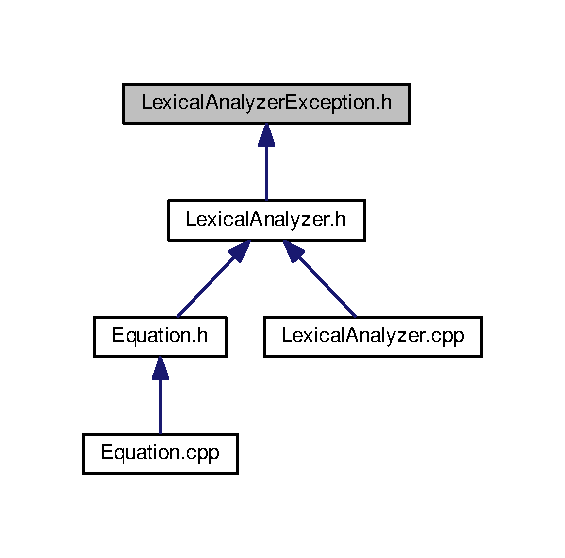
\includegraphics[width=271pt]{_lexical_analyzer_exception_8h__dep__incl}
\end{center}
\end{figure}
\subsection*{Classes}
\begin{DoxyCompactItemize}
\item 
class \hyperlink{classteam22_1_1_calc_1_1_lexical_analyzer_exception}{team22\+::\+Calc\+::\+Lexical\+Analyzer\+Exception}
\end{DoxyCompactItemize}
\subsection*{Namespaces}
\begin{DoxyCompactItemize}
\item 
 \hyperlink{namespaceteam22_1_1_calc}{team22\+::\+Calc}
\end{DoxyCompactItemize}


\subsection{Detailed Description}
U\+T\+F-\/8 \begin{DoxyDate}{Date}
25.\+3.\+18 
\end{DoxyDate}
\begin{DoxyAuthor}{Author}
Adam Mátl \href{mailto:xmatla00@stud.fit.vutbr.cz}{\tt xmatla00@stud.\+fit.\+vutbr.\+cz} \href{mailto:matla@matla.cz}{\tt matla@matla.\+cz} 
\end{DoxyAuthor}

\hypertarget{_lex_identification_observer_8h}{}\section{Lex\+Identification\+Observer.\+h File Reference}
\label{_lex_identification_observer_8h}\index{Lex\+Identification\+Observer.\+h@{Lex\+Identification\+Observer.\+h}}
{\ttfamily \#include \char`\"{}Lex.\+h\char`\"{}}\newline
Include dependency graph for Lex\+Identification\+Observer.\+h\+:
\nopagebreak
\begin{figure}[H]
\begin{center}
\leavevmode
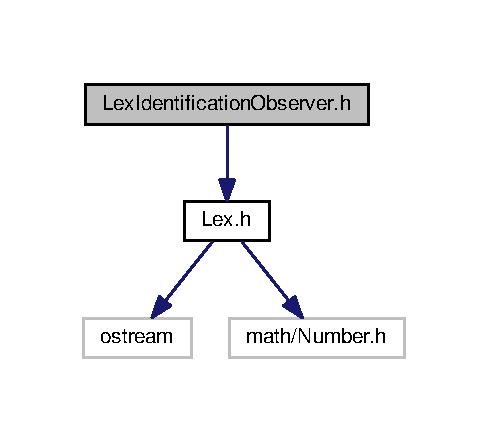
\includegraphics[width=291pt]{_lex_identification_observer_8h__incl}
\end{center}
\end{figure}
This graph shows which files directly or indirectly include this file\+:
\nopagebreak
\begin{figure}[H]
\begin{center}
\leavevmode
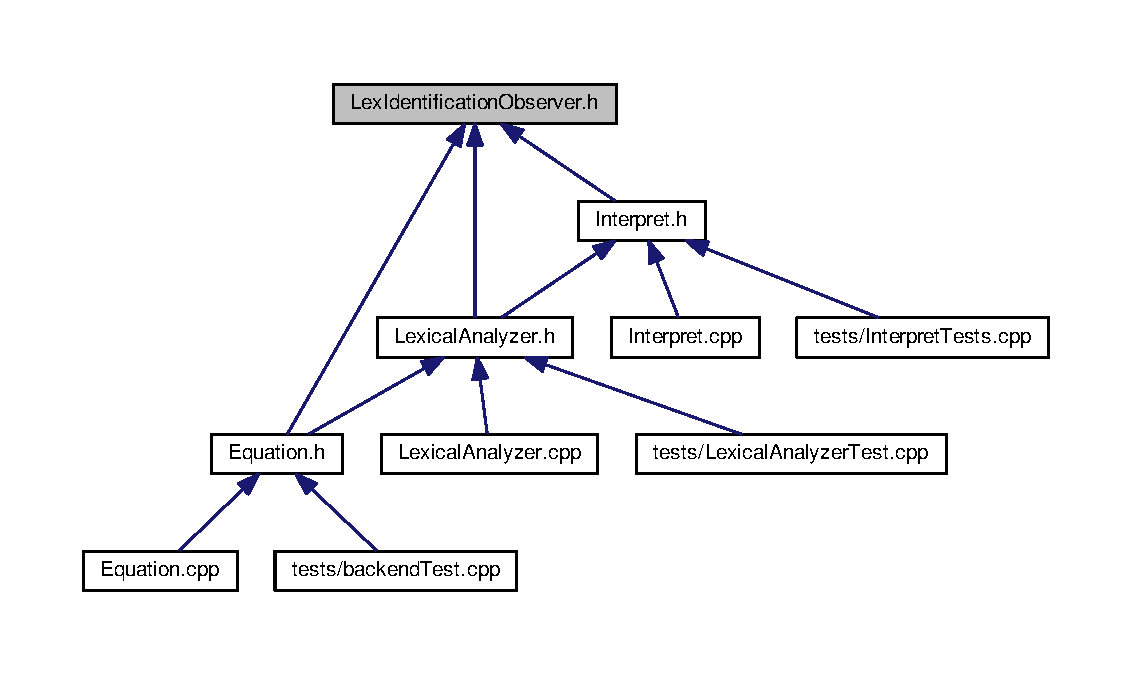
\includegraphics[width=350pt]{_lex_identification_observer_8h__dep__incl}
\end{center}
\end{figure}
\subsection*{Classes}
\begin{DoxyCompactItemize}
\item 
class \hyperlink{classteam22_1_1_calc_1_1_lex_identification_observer}{team22\+::\+Calc\+::\+Lex\+Identification\+Observer}
\end{DoxyCompactItemize}
\subsection*{Namespaces}
\begin{DoxyCompactItemize}
\item 
 \hyperlink{namespaceteam22_1_1_calc}{team22\+::\+Calc}
\end{DoxyCompactItemize}

\hypertarget{main_8cpp}{}\section{src/main.cpp File Reference}
\label{main_8cpp}\index{src/main.\+cpp@{src/main.\+cpp}}
{\ttfamily \#include $<$Q\+Application$>$}\newline
{\ttfamily \#include $<$Q\+Qml\+Application\+Engine$>$}\newline
{\ttfamily \#include $<$Qt\+Qml$>$}\newline
Include dependency graph for main.\+cpp\+:
\nopagebreak
\begin{figure}[H]
\begin{center}
\leavevmode
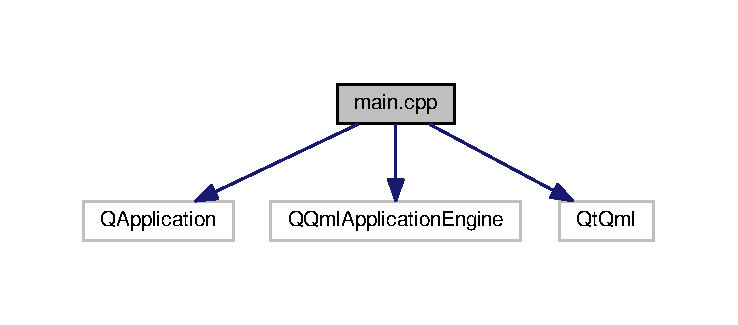
\includegraphics[width=350pt]{main_8cpp__incl}
\end{center}
\end{figure}
\subsection*{Functions}
\begin{DoxyCompactItemize}
\item 
int \hyperlink{main_8cpp_a0ddf1224851353fc92bfbff6f499fa97}{main} (int argc, char $\ast$argv\mbox{[}$\,$\mbox{]})
\end{DoxyCompactItemize}


\subsection{Function Documentation}
\mbox{\Hypertarget{main_8cpp_a0ddf1224851353fc92bfbff6f499fa97}\label{main_8cpp_a0ddf1224851353fc92bfbff6f499fa97}} 
\index{main.\+cpp@{main.\+cpp}!main@{main}}
\index{main@{main}!main.\+cpp@{main.\+cpp}}
\subsubsection{\texorpdfstring{main()}{main()}}
{\footnotesize\ttfamily int main (\begin{DoxyParamCaption}\item[{int}]{argc,  }\item[{char $\ast$}]{argv\mbox{[}$\,$\mbox{]} }\end{DoxyParamCaption})}



Definition at line 5 of file main.\+cpp.


\hypertarget{_result_observer_8h}{}\section{Result\+Observer.\+h File Reference}
\label{_result_observer_8h}\index{Result\+Observer.\+h@{Result\+Observer.\+h}}
{\ttfamily \#include \char`\"{}math/\+Number.\+h\char`\"{}}\newline
{\ttfamily \#include \char`\"{}Interpret\+Exception.\+h\char`\"{}}\newline
Include dependency graph for Result\+Observer.\+h\+:
\nopagebreak
\begin{figure}[H]
\begin{center}
\leavevmode
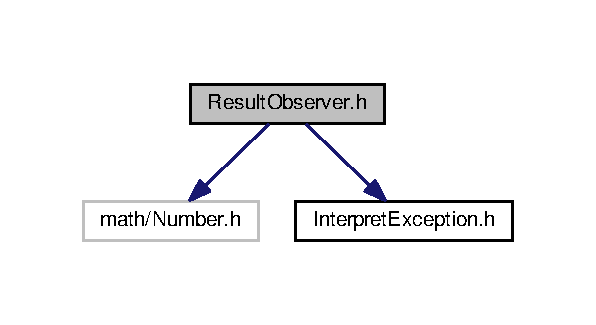
\includegraphics[width=333pt]{_result_observer_8h__incl}
\end{center}
\end{figure}
This graph shows which files directly or indirectly include this file\+:
\nopagebreak
\begin{figure}[H]
\begin{center}
\leavevmode
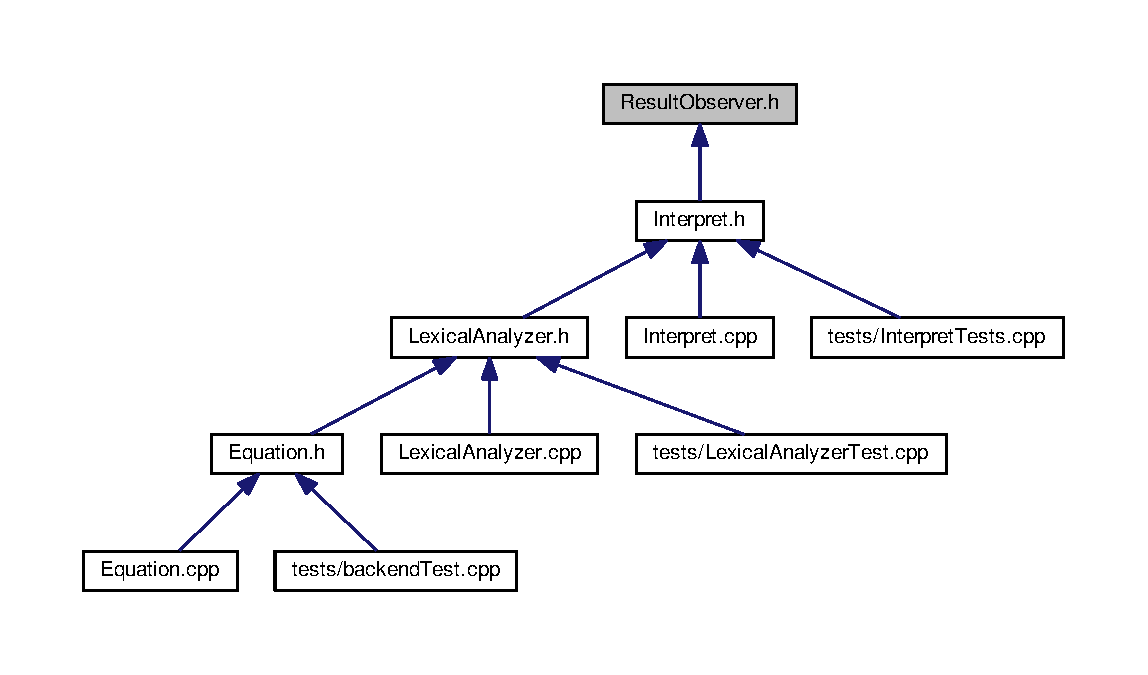
\includegraphics[width=350pt]{_result_observer_8h__dep__incl}
\end{center}
\end{figure}
\subsection*{Classes}
\begin{DoxyCompactItemize}
\item 
class \hyperlink{classteam22_1_1_calc_1_1_result_observer}{team22\+::\+Calc\+::\+Result\+Observer}
\end{DoxyCompactItemize}
\subsection*{Namespaces}
\begin{DoxyCompactItemize}
\item 
 \hyperlink{namespaceteam22_1_1_calc}{team22\+::\+Calc}
\end{DoxyCompactItemize}


\subsection{Detailed Description}
U\+T\+F-\/8 \begin{DoxyDate}{Date}
29.\+3.\+18 
\end{DoxyDate}
\begin{DoxyAuthor}{Author}
Adam Mátl \href{mailto:xmatla00@stud.fit.vutbr.cz}{\tt xmatla00@stud.\+fit.\+vutbr.\+cz} \href{mailto:matla@matla.cz}{\tt matla@matla.\+cz} 
\end{DoxyAuthor}

\chapter{Example Documentation}
\hypertarget{_2root_2_documents_2_git_clone_2_f_i_t__i_v_s__p_r_o_j_e_c_t2_2src_2_interpret_8h-example}{}\section{/root/\+Documents/\+Git\+Clone/\+F\+I\+T\+\_\+\+I\+V\+S\+\_\+\+P\+R\+O\+J\+E\+C\+T2/src/\+Interpret.\+h}
Po přijetí min počtu lexemů pro interpretaci je interpretace provedena a výsledek předá pomocí callbacku {\ttfamily Result\+Observer\+::on\+Result\+Change}. Objekty na kterých bude callback volán lze registrovat pomocí {\ttfamily Interpret\+::registr\+Result\+Callback}

Lexem {\ttfamily Lex\+::\+E\+V\+AL} po eval pokud příjde číslo přepíše výsledek číslem, pokud operator stejné chování jako eval nepřišlo

Lexemi {\ttfamily Lex\+::\+BS} a {\ttfamily Lex\+::\+C\+L\+E\+AR} provedou vynulování výsledku (a notifikaci o změně)

Ostatní lexémy budou vyhodnoceny jako matematické operace

Pořadí provázení operací je totožné s pořadím jejich předání. Pokud sekvence začíná operátorem předpokládá se první operátor 0

Pokud je předaná chybná sekvence lexému je oznámena chyba callback {\ttfamily Result\+Observer\+::on\+Error}.

Auto i = Interpret; i.\+send\+Identified\+Lex(\+Number(5)); // Informování o změně výsledků na 5 pomocí callbacků i.\+send\+Identified\+Lex(\+Lex(\+Lex\+::\+A\+D\+D)); i.\+send\+Identified\+Lex(\+Number(4)); // Provedení operace =$>$ 5+4 výsledek 9 // Informování o změně výsledků na 9 pomocí callbacků i.\+send\+Identified\+Lex(\+Lex(\+Lex\+::\+A\+D\+D)); i.\+send\+Identified\+Lex(\+Number(4)); // Provedení operace =$>$ (předchozí výsledek)9+4 výsledek 13 // Informování o změně výsledků na 13 pomocí callbacků


\begin{DoxyCodeInclude}

\textcolor{preprocessor}{#ifndef FIT\_IVS\_PROJECT2\_INTERPRET\_H}
\textcolor{preprocessor}{#define FIT\_IVS\_PROJECT2\_INTERPRET\_H}

\textcolor{preprocessor}{#include <set>}
\textcolor{preprocessor}{#include "\hyperlink{_lex_identification_observer_8h}{LexIdentificationObserver.h}"}
\textcolor{preprocessor}{#include "\hyperlink{_lex_8h}{Lex.h}"}
\textcolor{preprocessor}{#include "\hyperlink{_result_observer_8h}{ResultObserver.h}"}
\textcolor{preprocessor}{#include "\hyperlink{_number_8h}{math/Number.h}"}
\textcolor{keyword}{namespace }\hyperlink{namespaceteam22_1_1_calc}{team22::Calc}
\{
\textcolor{keyword}{class }Interpret: \textcolor{keyword}{public} LexIdentificationObserver
\{
    \textcolor{keywordtype}{void} \hyperlink{classteam22_1_1_calc_1_1_interpret_af38e3b867c32f50c921027249fc1185a}{notifyResultChanged}();

    \textcolor{keywordtype}{void} \hyperlink{classteam22_1_1_calc_1_1_interpret_ab9db5790b1aab8a3f315296853c8e9c6}{notifyAboutError}(\hyperlink{class_interpret_exception}{InterpretException} exception);

\textcolor{keyword}{public}:
    std::set<ResultObserver *> \hyperlink{classteam22_1_1_calc_1_1_interpret_a7db1e80a4733124ed425e62a90f9eadb}{resultCallbackObjects};

    \textcolor{keywordtype}{void} \hyperlink{classteam22_1_1_calc_1_1_interpret_a23e1e307b4f7ffd42f8eb31d33314c41}{registrResultCallback}(ResultObserver *resultCallbackObject);

    \textcolor{keywordtype}{void} \hyperlink{classteam22_1_1_calc_1_1_interpret_a479c65c010f4ef1060049b684e5f7eb6}{sendIdentifiedLex}(Lex lex) \textcolor{keyword}{override};
\};
\}


\textcolor{preprocessor}{#endif //FIT\_IVS\_PROJECT2\_INTERPRET\_H}
\end{DoxyCodeInclude}
 
%--- End generated contents ---

% Index
\backmatter
\newpage
\phantomsection
\clearemptydoublepage
\addcontentsline{toc}{chapter}{Index}
\printindex

\end{document}
